
%----------------------------------------------------------------------------------------
% Impresión de un lado de la hoja
\documentclass[notitlepage]{report}
\usepackage[paper=a4paper,top=2in, bottom=1in, left=1in, right=1in]{geometry}

%----------------------------------------------------------------------------------------
% Impresión para libros (de los dos lados de la hoja)
%\documentclass[a4paper,twoside, notitlepage]{report}
%----------------------------------------------------------------------------------------
% PAQUETES NECESARIOS
\usepackage[utf8]{inputenc} % set input encoding
\usepackage{amsmath}
\usepackage{amssymb} %para mathbb
\usepackage{eqnarray}
\usepackage{bm}
\usepackage{mathtools}
\usepackage{xcolor}
\usepackage{xfrac}
\usepackage{esint}
\usepackage{mathcomp}
\usepackage[rightcaption]{sidecap}
\usepackage{graphicx} 
\usepackage{array}
\usepackage{todonotes}
\newenvironment{conditions}
  {\par\vspace{\abovedisplayskip}\noindent\begin{tabular}{>{$}l<{$} @{${}={}$} l}}
  {\end{tabular}\par\vspace{\belowdisplayskip}}% necesario para agregar gráficos.
\usepackage[margin=2cm]{caption}  		% por defecto 2cm
\usepackage[spanish]{babel}
\usepackage[hidelinks]{hyperref}
\usepackage{afterpage}
\usepackage{tikz}
\usepackage{fancyhdr}
\usepackage{acro} 
\usepackage[lined,ruled,vlined,linesnumbered,spanish, onelanguage]{algorithm2e}
\usepackage{listings}

% Anexos y readecuación de nombres.
\usepackage[toc,page]{appendix}
\addto\captionsspanish{%
	\renewcommand\appendixname{Anexo}
	\renewcommand\appendixpagename{Anexos}
	\renewcommand\appendixtocname{Anexos}
}
%----------------------------------------------------------------------------------------
% CONFIGURACIÓN INTERLÍNEA. 
% Quitar el comentario a \usepackage{setspace} y 
% seleccionar alguna de las opciones (quitar % a la elegida)
% \usepackage{setspace}

% Opciones:
%\doublespacing
%\onehalfspacing
%\singlespace
%----------------------------------------------------------------------------------------
% Estilo para encabezado de página
\pagestyle{fancy}
\fancyhf{}
\fancyhead[L]{\bfseries\leftmark} % Título
\fancyhead[R]{\bfseries\thepage}  % Nro de página
\renewcommand\headrulewidth{0pt}  % línea 
%----------------------------------------------------------------------------------------
% Algunos colores de diseño
\definecolor{hyperlink}{rgb}{0,0,93.3}
\definecolor{ideicolor}{RGB}{139, 13, 51}

%============================================================
% DEFINICIÓN DE COMANDOS PARA CARGA DE DATOS
\NewDocumentCommand{\universidad}{m}{\newcommand{\univn}{#1}}
\NewDocumentCommand{\instituto}{m}{\newcommand{\instn}{#1}}
\NewDocumentCommand{\autor}{m}{\newcommand{\autorn}{#1}}
\NewDocumentCommand{\coautor}{m}{\newcommand{\coautorn}{#1}}
\NewDocumentCommand{\autormail}{m}{\newcommand{\autorm}{#1}}
\NewDocumentCommand{\coautormail}{m}{\newcommand{\coautorm}{#1}}
\NewDocumentCommand{\supervisor}{m}{\newcommand{\supname}{#1}}
\NewDocumentCommand{\cosupervisor}{m}{\newcommand{\cosupname}{#1}}
\NewDocumentCommand{\examiner}{m}{\newcommand{\examname}{#1}}
\NewDocumentCommand{\grado}{m}{\newcommand{\gradon}{#1}}
\NewDocumentCommand{\grupo}{m}{\newcommand{\grupon}{#1}}
\NewDocumentCommand{\subject}{m}{\newcommand{\subjectname}{#1}}
\NewDocumentCommand{\keywords}{m}{\newcommand{\keywordnames}{#1}}
\NewDocumentCommand{\titulo}{m}{\newcommand{\ttitle}{#1}}

%============================================================
% Algunos formatos nuevos para separar el formato del contexto
\newcommand{\keyword}[1]{\textbf{#1}}
\newcommand{\tabhead}[1]{\textbf{#1}}
\newcommand{\code}[1]{\texttt{#1}}
\newcommand{\file}[1]{\texttt{\bfseries#1}}
\newcommand{\option}[1]{\texttt{\itshape#1}}
\newcommand\blankpage{
	\null
	\thispagestyle{empty}
	\addtocounter{page}{0}
	\newpage}
%================================================================
% Estilado codigo tesina

\definecolor{codegreen}{rgb}{0,0.6,0}
\definecolor{codegray}{rgb}{0.5,0.5,0.5}
\definecolor{codepurple}{rgb}{0.58,0,0.82}
\definecolor{backcolour}{rgb}{0.95,0.95,0.92}

\lstdefinestyle{codestyle}{
    backgroundcolor=\color{backcolour},   
    commentstyle=\color{codegreen},
    keywordstyle=\color{magenta},
    numberstyle=\tiny\color{codegray},
    stringstyle=\color{codepurple},
    basicstyle=\ttfamily\footnotesize,
    breakatwhitespace=false,         
    breaklines=true,                 
    captionpos=b,                    
    keepspaces=true,                 
    numbers=left,                    
    numbersep=5pt,                  
    showspaces=false,                
    showstringspaces=false,
    showtabs=false,                  
    tabsize=2
}


%================================================================
% DATOS DE  PORTADA
%----------------------------------------------------------------------------------------
% Datos Institucionales.
\universidad{	\href{www.ungs.edu.ar}{Universidad Nacional de General Sarmiento}}
\instituto{\href{https://www.ungs.edu.ar/idei/idei}{Instituto de Industria (IDEI)}}
%----------------------------------------------------------------------------------------
% Datos Particulares
\titulo{\vspace{-4.5cm} Rastreo de dispositivos móviles mediante el uso de paquetes de control 802.11 con dispositivos de baja potencia }
% Grado Alcanzado
\grado{Licenciado en Sistemas} % Cambiar según corresponda (a/o/os/as)
%Autorres
\autor{Agustin C. Alexander}
\autormail{agustin.c.alexander@gmail.com}
% Gupo de Investigación o Laboratorio. (si fuera necesario declarar, quitar ~ y reemplazar por el nombre)
\grupo{~} 
%Directores, Supervisores.
\supervisor{Alexis Tcach Lufrano}

%===========================================================================
%DECLARACIÓN DE ACRÓNIMOS Y GLOSARIO
%----------------------------------------------------------------------------------------
% Los Acrónimos y Glosario de terminos se declara en el encabezado (previo al cuerpo del documento)
% Se emplea el paquete "acro" : https://github.com/cgnieder/acro/
% Hay ciertas incompatibilidades entre diferentes compiladores de latex 
% principalmente por el versionado.   .
%----------------------------------------------------------------------------------------
%% Con LiveTex ()LINUX)
%% class 'abbrev':abreviaciones:

%% class 'nomencl':glosario
% For the glossary (nomenclature)

\DeclareAcronym{rssi}{
    short = RSSI,
    long = \textit{Received Signal Strength Indicator},
    sort = a,
    class = abbrev
}
\DeclareAcronym{ssid}{
	short = SSID,
	long  = \textit{Service Set Identifier},
	sort  = ssid,
	class = abbrev
}
\DeclareAcronym{wpa2}{
	short = WPA2,
	long  = \textit{Wi-Fi Protected Access 2},
	sort  = wpa2,
	class = abbrev
}
\DeclareAcronym{wpa3}{
	short = WPA3,
	long  = \textit{Wi-Fi Protected Access 3},
	sort  = wpa3,
	class = abbrev
}
\DeclareAcronym{bssid}{
	short = BSSID,
	long  = \textit{Basic Service Set Identifier},
	sort  = ssid,
	class = abbrev
}
\DeclareAcronym{gps}{
	short = GPS,
	long  = \textit{Global Positioning System},
	sort  = c,
	class = abbrev
}
\DeclareAcronym{sdk}{
	short = SDK,
	long  = \textit{Software Development Kit},
	sort  = d,
	class = abbrev
}
\DeclareAcronym{esp}{
	short = ESP8266,
	long  = \textit{Espressif System's Wi-Fi Microchip},
	sort  = e,
	class = abbrev
}
\DeclareAcronym{ble}{
	short = BLE,
	long  = \textit{Bluetooth Low Energy},
	sort  = f,
	class = abbrev
}
\DeclareAcronym{wifi}{
	short = Wi-Fi,
	long  = \textit{Wireless Fidelity},
	sort  = g,
	class = abbrev
}
\DeclareAcronym{dbm}{
	short = dBm,
	long  = \textit{Decibels relative to one milliwatt},
	sort  = h,
	class = abbrev
}
\DeclareAcronym{api}{
	short = API,
	long  = \textit{Application Programming Interface},
	sort  = i,
	class = abbrev
}
\DeclareAcronym{lan}{
	short = LAN,
	long  = \textit{Local Area Network},
	sort  = j,
	class = abbrev
}
\DeclareAcronym{wan}{
	short = WAN,
	long  = \textit{Wide Area Network},
	sort  = k,
	class = abbrev
}
\DeclareAcronym{lpwan}{
	short = LPWAN,
	long  = \textit{Low Power Wide Area Network},
	sort  = l,
	class = abbrev
}
\DeclareAcronym{lora}{
	short = LoRa,
	long  = \textit{Long Range},
	sort  = m,
	class = abbrev
}
\DeclareAcronym{nbiot}{
	short = NB-IoT,
	long  = \textit{Narrowband IoT},
	sort  = n,
	class = abbrev
}
\DeclareAcronym{beacons}{
	short = Beacon,
	long  = \textit{Beacon Frame},
	sort  = beacon,
	class = nomencl
}
\DeclareAcronym{prq}{
	short = PRQ,
	long  = \textit{Probe Request},
	sort  = prq,
	class = nomencl
}
\DeclareAcronym{prs}{
	short = PRS,
	long  = \textit{Probe Response},
	sort  = prs,
	class = nomencl
}
\DeclareAcronym{ap}{
	short = AP,
	long  = \textit{Access Point},
	sort  = o,
	class = abbrev
}
\DeclareAcronym{rpi}{
	short = RPI,
	long  = \textit{Raspberry Pi},
	sort  = rpi,
	class = abbrev
}
\DeclareAcronym{esp32}{
	short = ESP32,
	long  = \textit{Espressif Systems Wi-Fi + Bluetooth Microchip},
	sort  = esp32,
	class = abbrev
}
\DeclareAcronym{mac}{
	short = MAC,
	long  = \textit{Media Access Control Address},
	sort  = mac,
	class = abbrev
}
\DeclareAcronym{vin}{
	short = VIN,
	long  = \textit{Voltage In},
	sort  = vin,
	class = abbrev
}
\DeclareAcronym{gnd}{
	short = GND,
	long  = \textit{Ground},
	sort  = gnd,
	class = abbrev
}
\DeclareAcronym{sdcard}{
	short = SD,
	long  = \textit{Secure Digital Card},
	sort  = sdcard,
	class = abbrev
}
\DeclareAcronym{udp}{
	short = UDP,
	long  = \textit{User Datagram Protocol},
	sort  = udp,
	class = abbrev
}
\DeclareAcronym{csv}{
	short = CSV,
	long  = \textit{Comma-Separated Values},
	sort  = csv,
	class = abbrev
}
\DeclareAcronym{ip}{
	short = IP,
	long  = \textit{Internet Protocol},
	sort  = ip,
	class = abbrev
}
\DeclareAcronym{5g}{
	short = 5G,
	long  = \textit{Fifth Generation},
	sort  = 5g,
	class = abbrev
}
\DeclareAcronym{odv}{
    short = AODV,
    sort  = odv,
    long = \textit{Ad hoc On-Demand Distance Vector Routing},
    class = abbrev
}
\DeclareAcronym{ns3}{
    short = NS3,
    sort  = ns3,
    long = \textit{Network Simulator 3},
    class = abbrev
}
\DeclareAcronym{ungs}{
    short = UNGS,
    long = Universidad Nacional de General Sarmiento,
    class = abbrev
}
\DeclareAcronym{usb}{
    short = USB,
    long = \textit{Universal Serial Bus},
    class = abbrev
}
\DeclareAcronym{slsqp}{
    short = SLSQP,
    long = \textit{Sequential Least Squares Quadratic} Programming,
    class = abbrev
}

\DeclareAcronym{iot}{
    short = IOT,
    long = Internet of Things,
    class = abbrev
}

%% Con MikTex (Mac - Windows)
%%
%% tag 'abbrev':abreviaciones:
%\DeclareAcronym{id}{
%	short = I+D ,
%	long  = Investigación y Desarrollo,
%	tag = abbrev}

%% tag 'nomencl': glosario
%\DeclareAcronym{angelsperarea}{
%	short = \ensuremath{a} ,
%	long  = El número de ángeles por unidad de área ,
%	sort  = a ,
%	tag = nomencl}

%=======================================================================================
% DOCUMENTO DE TESIS
\begin{document}

% Numeración romana para las páginas preliminares
\pagenumbering{roman} 

%----------------------------------------------------------------------------------------
%  Título - PORTADA 
%----------------------------------------------------------------------------------------
\begin{titlepage}
	\begin{tikzpicture}[remember picture, overlay]
		\node[
		anchor=center,
		xshift=7.5cm,
		yshift=4cm,
		rectangle,
		%fill=gray!20!white,
		%fill opacity=0.8,
		inner ysep=5pt,
		inner xsep=3cm,
		%text opacity=0.8,
		%text width=\paperwidth+1cm, % Set text width in order to force left-alignment
		]{
\includegraphics[width=22cm]{Figuras/ungs.png}};
	
	\end{tikzpicture}

	\begin{center}
		\vspace{-1.5cm}
		{\scshape\LARGE \univn\par}
		\vspace{1.5cm} % University name
		\textsc{\Large Tesina de la Licenciatura de Sistemas}\\[1.5cm] % Tipo de tesis
		\hrule
		\vspace{6.0cm}
		{\huge \bfseries \ttitle\par} \vspace{1.4cm} % Título de la tesis
		\hrule
		\vspace*{.06\textheight}
		\begin{minipage}[t]{0.4\textwidth}
			\begin{flushleft} \large
				\emph{Autor:}\\
				\href{\autorm}{\autorn} \\ % Autor /a 
				% salto de línea necesario
				\href{\coautorm}{\coautorn} %  Coautor/a  
			\end{flushleft}
		\end{minipage}
		\begin{minipage}[t]{0.4\textwidth}
			\begin{flushright} \large
				\emph{Supervisor:} \\
				\supname
				
				% salto de línea necesario
				\cosupname
			\end{flushright}
		\end{minipage}\\[2cm]
		\vfill
		\large \textit{La tesina se presenta para cumplir con los requerimientos de grado de \\ \gradon}\\[0.3cm] % University requirement text
		\textit{en el}\\[0.4cm]
		{\color{ideicolor} \grupon \\ \LARGE \instn}\\[1cm] % Research group name and department name
		\vfill
		{\large \today}\\[4cm] % Date
		%\includegraphics{Logo} % University/department logo - uncomment to place it
		
		\vfill
	\end{center}
\end{titlepage}


%----------------------------------------------------------------------------------------
%	PÁGINA DE CITA, si el autor lo requiere
%----------------------------------------------------------------------------------------
\vspace*{0.1\textheight}

{\itshape Cuando se empieza a hablar en términos absolutos en la política, significa que las atrocidades están a punto de comenzar. La humanidad ha logrado cosas asombrosas simplemente avanzando a través de discusiones, quejas, luchas y negociaciones. Es caótico y poco digno, pero es cuando estamos en nuestra mejor forma, porque todos tienen la oportunidad de hacer competir su voz. Incluso si otros intentan constantemente callarla. Cuando solo una voz tiene la posibilidad de ser expresada, lo que suele surgir de eso puede ser algo terrible. }\bigbreak

\hfill Persepolis Rising - James S.A. Corey, 2017

\afterpage{\blankpage}
\clearpage

%--------------------------------------------------------------------------------------
%  RESUMEN
%--------------------------------------------------------------------------------------
\begin{abstract} 
	\addcontentsline{toc}{section}{Resumen}
	Existen múltiples organizaciones, como centros comerciales, que proveen Wi-Fi gratuito como incentivo para luego, aprovechando esa conexión, poder determinar el comportamiento de sus clientes; que negocios prefieren, cuánto tiempo pasan en el establecimiento y hasta que gondolas les interesa más. Esto requiere sin embargo de que los individuos decidan conectarse a dicho Wi-Fi\cite{Jordan2015ReliablePD}.
\newline
Nuestro trabajo consiste en investigar si existe la posibilidad de deducir el recorrido de transeúntes y vehículos usando un método similar sin necesidad de una conexión previa realizada por el usuario. Mas precisamente nos planteamos ver cuán factible es, utilizando dispositivos de bajo costo, estimar la posición y recorrido de un teléfono móvil sin necesidad de que este se encuentre conectado a una red Wi-Fi, es decir, de manera pasiva.
\newline
En este trabajo, describimos la implementación de un sistema de seguimiento que utiliza el RSSI (Received Signal Strength Indication) recibido a partir de sensores ESP8266, para inferir información de ubicación de un dispositivo móvil mediante paquetes de control 802.11. El sistema utiliza una red de puntos de referencia fijos, cada uno equipado con un sensor ESP8266, para medir la intensidad de las señales recibidas del dispositivo móvil y calcular su ubicación utilizando algoritmos de  multilateración. El bajo coste y la amplia disponibilidad de dichos sensores, así como su diseño de bajo consumo, los hacen muy adecuados para el despliegue masivo de una red de sensores urbana en particular para su uso en aplicaciones de rastreo de localización.
\newline
Como resultado, se logró desarrollar un sistema funcional de localización pasiva con pruebas exitosas en escenarios reales y simulados, junto con diversas herramientas de software publicadas. Incluyendo bibliotecas de multilateración, firmware personalizado, y entornos de simulación. Estas aydan a demostrar la viabilidad técnica de este enfoque para aplicaciones urbanas en el contexto de \textit{Smart Cities} y en particular el monitoreo del flujo urbano.
\end{abstract}

\afterpage{\blankpage}
\clearpage

%----------------------------------------------------------------------------------------
%	AGRADECIMIENTOS	
%----------------------------------------------------------------------------------------
\section*{Agradecimientos}
\addcontentsline{toc}{section}{Agradecimientos}
        Muchas gracias a Alexis Tcach y a Ivan Jourdan, quienes sin sus ideas y su guia este trabajo jamas hubiera sido posible. A Pedro Gutierrez, Sebastian Pintos, Bruno Capecce y Fernando Molachino por ayuda durante la fase experimental de este proyecto. Y finalmente a todos los que me incitaron a terminar este trabajo y me empujaron a mas.\ldots
\newpage

%-------------------------------------------------------------------------------------
%  INDICES
%-------------------------------------------------------------------------------------
% Lista de Abreviaciones
\printacronyms[include-classes=abbrev,name={\Huge Lista de abreviaciones \\}]   %TexLive
%\printacronyms[include=abbrev,name={\Huge Lista de Abreviaciones \\}]  % MikTex
\addcontentsline{toc}{section}{Lista de Abreviaciones}
\cleardoublepage
% Lista de Nomenclaturas
\printacronyms[include-classes=nomencl,name={\Huge  Glosario \\}]  %TexLive
%\printacronyms[include=nomencl,name={\Huge  Glosario \\}]  %MikTex
\addcontentsline{toc}{section}{Glosario}
% Lista de Figuras
\listoffigures
\addcontentsline{toc}{section}{Índice de Figuras}
% Lista de cuadros
\listoftables
\addcontentsline{toc}{section}{Índice de Cuadros}
% Índice
\renewcommand\headrulewidth{1pt} % a partir de aquí se tienen una línea en el header
\tableofcontents
\addcontentsline{toc}{section}{Índice General}

\clearpage

%----------------------------------------------------------------------------------------
%	DEDICATORIA	
%----------------------------------------------------------------------------------------
\chapter*{}
\addcontentsline{toc}{section}{Dedicatoria}
\vspace*{0.2\textheight}

\begin{center}{\Large\slshape Para mi Padre, Alfredo Carlos Alexander, quien despertó en mi desde muy temprano mi pasión por la ingeniería y gracias a quien elegí esta carrera. Y a mi madre, María Teresa Campos, quien ante cada obstaculo siempre me alentó a continuar en mis estudios.}\end{center}

\afterpage{\blankpage}
\clearpage
%----------------------------------------------------------------------------------------
% Numeración arábiga para el cuerpo de la tesis.
\pagenumbering{arabic} 
%-----------------------------------------------------------------------------------
% Capítulos 
%-----------------------------------------------------------------------------------
\chapter{Introducción}

\label{Capitulo_1} % Para referenciar el capítulo en el documento, usar \ref{Capitulo_1}
\section{Motivación y Antecedentes}
En el contexto de la planificación urbana y las ciudades inteligentes o \textit{Smart Cities}, el problema de encontrar espacios de estacionamiento es algo que se encuentra en estado de plena investigación y desarrollo. Se consultó la literatura y se encontró soluciones que utilizan sensores colocados en el pavimento o numerosas cámaras más algún tipo de software que permite detección de estacionamiento. Estas soluciones, si bien pueden ser efectivas, tienen como problema el uso de hardware costoso con gran poder de cómputo, cuya instalación requiere de gran esfuerzo y recursos.

Basándose en la experiencia previa adquirida durante la colaboración con el municipio de San Miguel en la investigación y desarrollo del proyecto \textit{Smart Cities} \cite{sedici89263}, el grupo de investigación en redes AD-HOC de la UNGS, se puso como objetivo el desarrollo de una solución de bajo costo para \textit{Smart Parking}.

Luego de analizar el estado del arte se concluyó que existía novedad y utilidad en un sistema \textit{wireless} de rastreo de vehículos y transeúntes. Este podría permitir a su vez en trabajos futuros identificar si un vehículo se encuentra en movimiento, detenido o ha estacionado.

Un sistema completo como el que el equipo de investigación se propone analizar, permitiría detectar individuos que posean dispositivos móviles o cualquier otro tipo de dispositivo que posea \acs{wifi} o incluso \acs{ble}. Una vez identificado, el sistema podrá ser capaz de detectar su ubicación a lo largo del tiempo y finalmente predecir si dicho dispositivo se encuentra dentro de un vehículo en movimiento, o es un transeúnte caminando, o bien es un vehículo que acaba de estacionar y a continuación marcar esa plaza como ocupada o detectar una zona que posee embotellamiento. Esta información es crucial para la administración de una ciudad que intenta introducirse al paradigma de \textit{Smart City} ya que le permitiría actuar de manera acorde ante estos eventos.

Por ejemplo, utilizando una aplicación de \textit{Smart Parking} sugerir al usuario dónde estacionar. Lo que es más, hasta podría permitirle a la ciudad, mediante el uso de dicha aplicación, ajustar las tarifas de estacionamiento según cuán congestionada se encuentre la zona. De esta manera permitiendo ahorro de combustible a los vehículos al no tener que recorrer mucha distancia para encontrar una plaza de estacionamiento y poder descomprimir los centros urbanos en horas de alta demanda.

Para que un dispositivo cliente se conecte a una red Wi-Fi, el primer paso es identificar los puntos de acceso (\acs{ap}) disponibles dentro de su rango. Este proceso utiliza dos tipos principales de tramas: los \acl{beacons}, enviados periódicamente por los \acs{ap}, y las \acl{prq}, que los clientes transmiten activamente cuando necesitan más información sobre las redes cercanas.

Los \acs{beacons} son señales que los \acs{ap} emiten a intervalos regulares, generalmente cada 100 ms, para anunciar la existencia de la red. Estas tramas incluyen datos esenciales como el nombre de la red (\acs{ssid}), la dirección MAC del punto de acceso (\acs{bssid}) y detalles técnicos sobre los canales, velocidades y métodos de cifrado soportados, como \acs{wpa2} o \acs{wpa3}. Este método permite a los dispositivos cliente identificar redes disponibles de manera pasiva, simplemente escuchando, lo cual es eficiente en términos de energía porque no implica que el cliente envíe datos.

En contraste, las \acl{prq} son tramas activas que los dispositivos cliente utilizan cuando necesitan información más específica o están buscando una red particular. Al enviar estas solicitudes, el cliente puede recibir respuestas de los \acs{ap} en el área, lo que resulta útil en escenarios como el roaming entre diferentes puntos de acceso o cuando el escaneo pasivo no es suficiente debido a interferencias o congestión.

Estos dos métodos, el escaneo pasivo mediante \acl{beacons} y el escaneo activo con \acl{prq}, se utilizan en conjunto para garantizar la detección y conexión a redes. Los \acl{beacons} reducen el consumo de energía al no requerir interacción activa, mientras que los \acl{prq} se adaptan a situaciones donde se requiere intervención activa. De esta manera, una vez descubierto el \acs{ap} se puede proceder con los siguientes pasos de la conexión wifi.


\section{Objetivo y alcance}
El presente trabajo investiga la viabilidad de estimar la ubicación y el recorrido de dispositivos móviles de manera pasiva, sin necesidad de que estos se encuentren conectados a una red \acs{wifi}. Para ello, se propone el uso de sensores de bajo costo basados en \acs{esp}, capaces de captar tramas de control 802.11 como los paquetes \acl{prq} y mediante el análisis del nivel de señal \acs{rssi} recibido en múltiples puntos, estimar la posición del dispositivo utilizando técnicas de multilateración. El sistema desarrollado demuestra que es posible realizar seguimiento pasivo de dispositivos móviles con precisión aceptable, lo cual abre la puerta a futuras aplicaciones de monitoreo urbano en entornos de \textit{Smart Cities}.

Como parte de esta línea de trabajo, se desarrolló un sistema funcional de localización pasiva que permite estimar la ubicación de dispositivos móviles sin requerir conexión previa. Además del sistema mismo, se desarrollaron una serie de herramientas complementarias publicadas como software libre, incluyendo firmware personalizado para los dispositivos embebidos utilizados, bibliotecas de multilateración y entornos de simulación. Estos recursos permiten tanto la reproducción de los experimentos como su adaptación a distintos escenarios urbanos.

Si bien el objetivo final del equipo de investigación es poder determinar con certeza el recorrido que realiza un vehículo al buscar estacionamiento en una ciudad.
Este trabajo se limita al objetivo investigar si existe la posibilidad de identificar el comportamiento de transeúntes sin necesidad de una conexión previa realizada por el usuario. Más precisamente nos planteamos ver cuán factible es, utilizando dispositivos de bajo costo, estimar la posición y recorrido de un teléfono móvil transportado por un individuo sin necesidad de que este se encuentre conectado, es decir, de manera pasiva. El seguimiento móvil mediante \acs{rssi} o \acl{rssi} y sensores \acs{esp} se planteó como una solución de bajo costo para determinar la ubicación de un dispositivo móvil.

Para tener resultados consistentes y poder saber a ciencia cierta si nuestro sistema era viable y poder plantear experimentos sencillos. Se tomó la decisión de realizar la conexión con el dispositivo móvil de manera diferente a en el escenario ideal donde el dueño del dispositivo no realiza ninguna modificación en la configuración de este y aún así es posible rastrearlo. La modificación realizada, fue encender el modo \acs{ap} \acs{wifi} del teléfono. Esto nos permite aumentar la frecuencia de envío de paquetes de tipo \acl{prq}. Exploraremos el motivo y los mecanismos más adelante, sin embargo este mismo sistema puede funcionar sin intervención del dispositivo rastreado si se quisiera aunque con menor frecuencia de envío.
\newline
A continuación, describimos la implementación de un sistema de seguimiento móvil que utiliza el \acs{rssi} recibido a partir de microcontroladores \acs{esp}, para inferir información de ubicación de un dispositivo móvil mediante paquetes de control 802.11. El sistema utiliza una red de puntos de referencia fijos, cada uno equipado con un \acs{esp}, para medir la intensidad de las señales recibidas del dispositivo móvil y calcular su ubicación utilizando algoritmos de multilateración. El bajo coste y la amplia disponibilidad de dichos sensores, así como su diseño de bajo consumo, los hacen muy adecuados para su uso en aplicaciones de seguimiento de localización. Demostraremos la eficacia del sistema de seguimiento móvil mediante experimentos que evalúan su precisión.

\section{Estructura del trabajo}
Este trabajo se organiza de la siguiente manera: En el Capítulo \ref{Capitulo_1} se plantea la introducción. En el Capítulo \ref{Capitulo_2}, se realiza una revisión de la literatura sobre las tecnologías inalámbricas y las técnicas de posicionamiento. En el Capítulo \ref{ExperimentoSimulado} se describe un experimento simulado de perfilado y multilateración. El Capítulo \ref{ExperimentoReal} presenta un experimento de campo real, para el perfilado de señales \acs{wifi} y multilateración. En el Capítulo \ref{Cap_Errores}, se discuten las fuentes de errores y las posibles mejoras. Finalmente, en el Capítulo \ref{Capitulo_Conclusiones} se presentan las conclusiones y las recomendaciones para futuros trabajos. Los Apéndices contienen detalles adicionales sobre los experimentos y los resultados.
\chapter{Revisión de Literatura}
\label{Capitulo_2}
\label{Literatura}
\section{Conexiones inalámbricas}
\subsection{Tipos de conexiones inalámbricas}

Además de la conectividad \acs{wifi}, existen otras tecnologías inalámbricas ampliamente utilizadas en dispositivos móviles, ordenadores personales y dispositivos \acl{iot}. Entre estas, \acl{ble} (\acs{ble}), una variante de Bluetooth diseñada para un consumo de energía extremadamente bajo, es especialmente relevante para aplicaciones \acl{iot} debido a su eficiencia energética y capacidad para operar en dispositivos alimentados por baterías durante largos períodos.

Otra tecnología inalámbrica importante es Zigbee, que utiliza el protocolo IEEE 802.15.4 para crear redes de área personal de baja potencia. Zigbee es común en aplicaciones de automatización del hogar y \acl{iot}, proporcionando una solución eficaz para controlar dispositivos inteligentes dentro de un hogar o edificio.

Las redes celulares, incluyendo tecnologías como 4G LTE y 5G, también juegan un papel crucial en la conectividad inalámbrica, ofreciendo cobertura a gran escala y soporte para una amplia gama de servicios móviles e \acs{iot}. Estas redes permiten la conectividad de dispositivos móviles y \acl{iot} en movimiento, soportando aplicaciones que requieren movilidad y acceso a internet de alta velocidad.

Finalmente, el \acl{lpwan} (\acs{lpwan}), incluyendo tecnologías como \acl{lora} y \acl{nbiot}, proporciona soluciones para aplicaciones \acl{iot} que requieren comunicaciones a larga distancia y bajo consumo de energía. Estas redes son ideales para sensores y dispositivos \acl{iot} distribuidos a lo largo de áreas extensas, como en aplicaciones de monitoreo ambiental y agricultura inteligente.

Se eligió utilizar \acs{wifi} como la tecnología para este sistema de seguimiento debido a varias razones prácticas. En primer lugar, la tecnología \acs{wifi} está presente en casi todos los teléfonos y muchos otros dispositivos, hasta incluso algunos autos. No hay necesidad de equipo extra o configuraciones especiales para detectar estos dispositivos, lo que lo hace muy accesible. Además, \acs{wifi} tiene un alcance más largo en comparación con tecnologías como Bluetooth, lo que permite cubrir áreas más grandes sin complicaciones. Otro punto a favor es que los dispositivos suelen buscar redes \acs{wifi} automáticamente, enviando solicitudes de sondeo de manera pasiva. Esto significa que se pueden rastrear sin que hagan algo activamente para ser detectados; esto convierte al \acs{wifi} en una tecnología ideal para monitorear movimientos y presencia en diversos entornos.

\subsection{Estados de conexión Wi-Fi}

Todos los dispositivos móviles, ordenadores personales y dispositivos \emph{IOT} que poseen conectividad Wi-Fi utilizan los mismos mecanismos de conexión. El esquema más común de topología de red es un \emph{Access Point} y múltiples dispositivos en modo cliente conectados a este. Por ejemplo, una laptop conectada a un router hogareño que le provee de internet.

\begin{figure}[!htb]
	\centering
	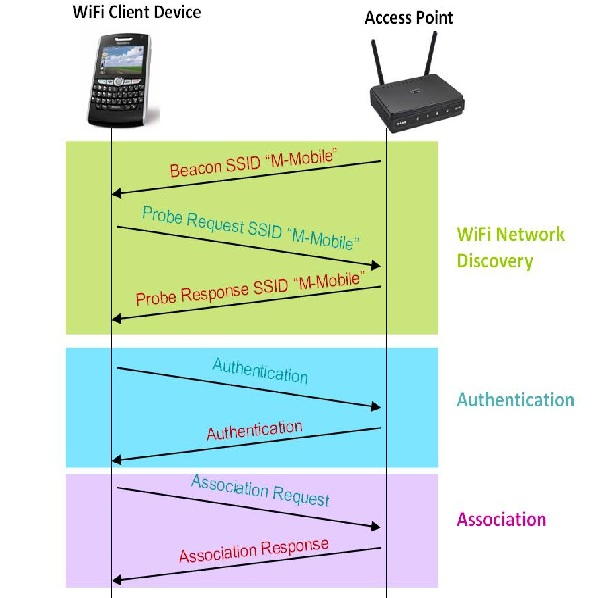
\includegraphics[width=0.6\textwidth]{Figuras/fig1.jpg}
	\captionsetup{margin=2cm}
	\caption[Secuencia de estado de la conexión]{Secuencia de estado de la conexión. Los paquetes de tipo Probe-Request o Beacon pertenecen a frames de clase 1. }
	\label{fig:frame-type}
\end{figure}

Si un dispositivo en modo cliente intenta conectarse a un \emph{Access Point} primero debe encontrarse en rango. Para saber que \emph{Access Points} están en rango para poder intentar la conexión, se utilizan dos paquetes que cumplen la misma función, pero lo realizan de maneras diferentes: Un paquete de tipo \emph{Probe Request} y un paquete \emph{Beacon}.

Un \emph{Beacon} es un tipo de paquete que emiten los \emph{Access Points} y tiene como objetivo anunciar a los clientes cercanos para que estos intenten conectarse si así lo desean. Un \emph{Probe Request} en cambio, es un paquete emitido por un cliente para solicitar información acerca de un \emph{Access Points} en particular o de todos los que se encuentren disponibles en un canal (banda inalámbrica para una frecuencia, ej., 2.4 GHz o 5 GHz).

Si un adaptador \acs{wifi} se encuentra en modo “promiscuo” o \emph{Sniffer}, podrá escuchar todos los paquetes y no solamente los que están dirigidos a dicho adaptador. Esto nos permitirá realizar una escucha pasiva, como mencionamos anteriormente. Por ende, un adaptador en dicho modo podrá recibir paquetes de todo tipo en particular, \emph{Probe-Request} de clientes y \emph{Beacon Frames}, de \emph{Access Points} respectivamente, que se encuentren en rango. 

Un cliente posee dos maneras de realizar un escaneo del área y determinar que \emph{Access Points} se encuentran presentes: un escaneo pasivo o un escaneo activo. 

Un escaneo pasivo (similar a un esquema de polling) consiste en sintonizar la antena de nuestro \emph{Sniffer} una fracción de tiempo a la vez en distintos canales (channel hopping). En cada canal se reciben \emph{Beacon Frames} pudiendo analizar así los \emph{Access Points} cercanos. 

Un escaneo activo, en cambio, envía \emph{Probe Request Frames} y espera \emph{Probe Response Frames} también usando opcionalmente \emph{Channel Hopping}. Esta estrategia es utilizada ampliamente por dispositivos móviles donde la batería es un factor a tener en cuenta y cuanto menos tiempo se necesite estar haciendo un escaneo, ya sea activo o pasivo, del área, mejor para el ahorro de energía del dispositivo en cuestión.

Entonces, de esta manera, un dispositivo podría activamente solicitar respuesta de un \emph{Access Point} en particular o de cualquiera en el área en vez de esperar a recibir un \emph{Beacon Frame}. Esto es beneficioso además, ya que asegura que ese \emph{Access Point} está en rango efectivo, ya que este pudo enviar su \emph{Probe Response} al cliente y este fue recibido exitosamente \cite{IEEE80211-2016}\cite{tanenbaum2011computer}.

\section{Técnicas de Posicionamiento}
\subsection{Intensidad de la Señal WiFi}

Para poder obtener la distancia a la que se encuentra un dispositivo inalámbrico, existen múltiples estrategias \cite{8692423} \cite{10.1007/1-4020-8155-3_8}. Una es enviar un mensaje (\emph{Ping}) y esperar la respuesta (\emph{Pong}). Con base en la diferencia entre el tiempo de emisión y el de respuesta, determinar la distancia según la velocidad de propagación de la onda electromagnética en el aire en promedio. Esta estrategia tiene el inconveniente de que sí requiere la cooperación del dispositivo del cual quiero obtener su posición, ya que necesito de su respuesta.

La otra alternativa es esperar a que el dispositivo inalámbrico cliente emita un paquete y medir su \acl{rssi} o \acs{rssi}. Este indicador representa una aproximación de la intensidad con la cual la antena inalámbrica receptora recibe el mensaje transmitido. Suele usarse a menudo en redes inalámbricas para determinar la calidad de la conexión entre dispositivos, pero puede aprovecharse para deducir su distancia (aplicando técnicas de predicción de la propagación del espectro electromagnético), como demuestra el estudio realizado por Barai et al. \cite{Barai2017EstimateDM}.

 Esta característica puede ser usada para, por ejemplo, visualizar la intensidad de la señal de los \emph{Access Point}\textit{s} que se encuentran en la cercanía, pero también sirve para que los \emph{Access Point}\textit{s} puedan saber la distancia a la que se encuentran sus clientes.

 

\subsection{Multilateración y Trilateración}

\begin{figure}[!htb]
	\centering
	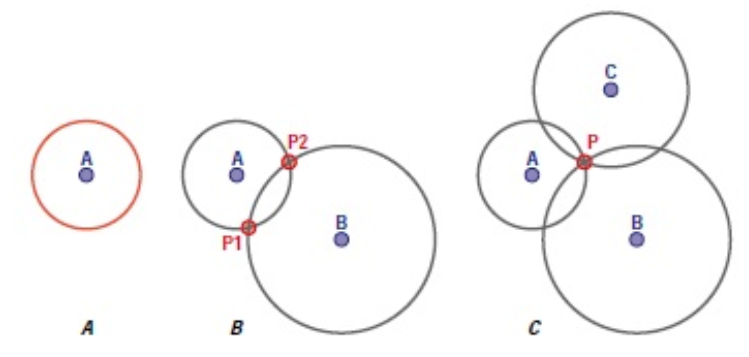
\includegraphics[width=0.7\textwidth]{Figuras/fig4.png}
	\captionsetup{margin=2cm}
	\caption[Casos Trilateración]{ Tipos de intersecciones. Utilizando el método clásico de trilateración, se pueden observar por lo menos tres casos.}
	\label{fig:tri}
\end{figure}

 Utilizando un \emph{Sniffer} para recibir los paquetes de tipo \acl{prq} o \emph{Beacon Frame} que se encuentran en un área y obteniendo el \acs{rssi} de cada paquete, es posible estimar la distancia a la que se encuentra un objetivo desde nuestro \emph{Sniffer} (caso A). Sin embargo, si se tiene más de un \emph{Sniffer} (B y C) y de cada uno conozco su ubicación precisa, puede entonces estimar la posición geográfica del cliente mediante multilateración.

La trilateración y la multilateración son técnicas matemáticas que se utilizan para determinar las coordenadas desconocidas de un punto en el espacio, basándose en las distancias desde ese punto a varios puntos conocidos. En el caso del GPS, un receptor mide la diferencia en el tiempo de llegada de las señales de al menos cuatro satélites, lo que permite calcular su posición tridimensional (latitud, longitud y altitud). De manera similar, en un entorno de localización basado en \acs{wifi}, los puntos conocidos serían los sensores \acs{wifi} que registran la presencia de otros dispositivos, y la ubicación desconocida sería la del dispositivo objetivo \cite{bulusu2000gps}.

La figura \ref{fig:tri} ilustra el concepto de trilateración, que es la base para entender la multilateración. En un contexto ideal, con tres círculos que se intersectan en un único punto, se puede determinar la ubicación exacta del dispositivo. Sin embargo, en la práctica, debido a factores como la interferencia de señales, los reflejos y la atenuación, las estimaciones de distancia basadas en \acs{rssi} pueden no ser precisas \cite{rappaport2002wireless}, lo que lleva a la necesidad de utilizar múltiples mediciones y aplicar técnicas de optimización para encontrar la mejor estimación de la posición\cite{ouyang2010received}\cite{li2012kalman}.

La multilateración es un proceso avanzado de localización que extiende los principios de la trilateración para estimar la posición de un objeto en dos o tres dimensiones. Mientras que la trilateración se basa en las distancias medidas desde tres puntos conocidos (en 2D) o cuatro puntos (en 3D) hasta el punto de interés, la multilateración utiliza señales de cuatro o más puntos para realizar la estimación, lo que mejora significativamente la precisión y la fiabilidad de la localización, especialmente en entornos complejos.

El proceso de multilateración implica la resolución de un sistema de ecuaciones que representan las distancias estimadas desde los nodos conocidos hasta el dispositivo. Este sistema puede ser linealizado y resuelto mediante el método de los cuadrados mínimos, como veremos más adelante en la sección \ref{sec:lsq}, para encontrar la ubicación que mejor se ajuste a las mediciones observadas. 

Entonces, hasta ahora podemos identificar a un dispositivo en particular y si se encuentra en rango de al menos uno de nuestros sensores que 

A partir de ahora llamaremos \emph{Sniffers} y sabremos su ubicación con mayor o menor precisión según cuantos \emph{Sniffers} tengamos en el área. Para poder seguir efectivamente la trayectoria de un individuo, es necesario poder identificar inequívocamente al dispositivo que se quiere rastrear a lo largo del tiempo. Esto es posible ya que cada paquete \emph{Probe Request} y \emph{Beacon Frame} contiene la \textit{\acs{mac} Address} del dispositivo que sirve como identificador único. 

\subsection{ Aleatorización de MAC Addresses}

Existen dispositivos que implementan técnicas de randomización de direcciones \acs{mac} \cite{martin2017study}; en este caso, se asigna periódicamente una dirección \acs{mac} aleatoria como medida de protección de la privacidad. Esta práctica complica el seguimiento continuo de dichos dispositivos y dificulta la estimación precisa del número de dispositivos presentes en una determinada área, puesto que el mismo dispositivo podría ser contabilizado en varias ocasiones bajo distintas direcciones \acs{mac}.

 Sin embargo, esta técnica no es aún ampliamente usada al momento de escribir este trabajo [1] e incluso se cuenta con la posibilidad de distinguir rápidamente si una \textit{\acs{mac} Address} es local (randomizada) o global (no randomizada) pudiendo así descartar “el ruido”.

Además, los dispositivos móviles \cite{freudiger2015talkative} suelen emitir los paquetes \acl{prq} en grandes ráfagas sin cambiar la \textit{\acs{mac} Address} incluso cuando estos tienen activada la randomización. Esto implica que, si bien no es posible saber en principio si es el mismo dispositivo el que desapareció de la ubicación anterior y luego reapareció en una nueva, al tener más de un \acl{prq} puedo saber su velocidad y dirección.

Lo que es más, sabiendo estos dos datos, es posible predecir que dos \textit{\acs{mac} Address} son distintas (randomizadas) sean en verdad pertenecientes al mismo dispositivo.

No obstante, aunque el dispositivo no randomice, es necesario para poder saber el recorrido completo de un dispositivo en un área, haciendo necesario algún tipo de algoritmo de predicción de desplazamiento. Ya que a no ser que todos los \emph{Sniffer}\textit{s} cubran el área en cuestión de manera completa, y no haya ninguna anomalía en la recepción. Van a haber secciones del recorrido que no van a poder ser capturadas por los \emph{Sniffer} ya sea por un problema de rango, de espacios ciegos, o bien porque el dispositivo cliente no emite la suficiente cantidad de \acl{prq} como para poder hacer un seguimiento más exhaustivo. Esto sin mencionar las anomalías de mediciones, ya sea por interferencia o por paredes en el medio que bajan la señal recibida a pesar de que el dispositivo no esté más lejos. 

En este trabajo, sin embargo, no exploramos el problema de la randomización ni el problema de los espacios ciegos. Nos limitaremos a ubicar en el espacio y el tiempo a un dispositivo en modo \emph{Access Point} emitiendo paquetes \emph{Beacon Frame}. De esta manera nos aislamos del problema de la randomización, además de tener una buena frecuencia regular de datos sin interrupciones, que es fundamental para los experimentos realizados.

\section{Medición de distancia en base al modelo de \textit{Path Loss}}

Para poder realizar el paso de multilateración, primero es necesario conocer la distancia desde cada uno de los \emph{Sniffer} hacia el \emph{“Objetivo”}. Para ello se usará en este trabajo la medición de \acs{rssi} y luego, para convertir de \acs{rssi} a distancia, basándonos en trabajos previos \cite{doi:10.4236/wsn.2010.28072} \cite{doi:10.1155/2014/371350}, se decidió usar un modelo derivado de la fórmula de pérdida en el trayecto de propagación o \emph{Path Loss}. Mediante el cual la pérdida de señal se incrementa proporcionalmente al logaritmo de la distancia recorrida.

Este modelo describe cómo la intensidad de una señal electromagnética disminuye a medida que se propaga a través del espacio. La pérdida ocurre debido a diversos factores como la dispersión, absorción y difracción de la señal, y se incrementa proporcionalmente a la distancia recorrida desde la fuente emisora. Esta atenuación de la señal es esencialmente una consecuencia de la expansión de las ondas electromagnéticas en el espacio, lo que resulta en una reducción de la densidad de potencia a medida que la distancia aumenta.

\newline
\newline

La fórmula general de \emph{Path Loss} en el espacio libre se puede expresar como:

\begin{equation}
    P(d)=P(d_{0}) - 10n*log(\frac{d}{d_{0}}) - X_{\sigma}
\end{equation}
Donde:
\begin{conditions}
 d         &  distancia (m)\\
 d_{0}   &  distancia de referencia inicial (m) \\
P(d)        &  es la potencia recibida en la distancia d \\
P(d_{0})   &  potencia en la distancia de referencia inicial (\acs{dbm}) \\
X_{\sigma} &  es una variable de ajuste que está relacionada directamente con la incertidumbre del modelo.\\
\end{conditions}
Luego podemos asumir que la distancia de referencia será 1 metro y agregar una variable A’ que ajustaremos para calibrar nuestra fórmula, reemplazando a \(P(d_{0})\) y \(X_{\sigma}\).
\begin{equation}
    RSSI = A' -10n*log(d)
\end{equation}
Finalmente, podemos simplificar aún más dividiendo por 10 y reemplazando \(A'/10\) por \(A\)
\begin{equation}
    RSSI = A - n*log(d)
\end{equation}

Ahora sólo resta hallar el valor de A y N para nuestros 

\emph{Sniffers} en el ambiente donde deseamos realizar la medición. Sin embargo, debido a las interferencias que ya mencionamos, en algunos escenarios puede ser necesario algún proceso que permita filtrar la señal para luego después proceder a hacer el siguiente paso de ajuste logarítmico.

\section{Ajuste Logarítmico}

El ajuste logarítmico juega un papel crucial en la modelización de la relación entre la intensidad de la señal recibida (\acs{rssi}) y la distancia en aplicaciones de localización y seguimiento. Este proceso implica ajustar un modelo matemático que mejor se acomode a los datos observados, permitiendo así predecir la distancia a partir de los valores de \acs{rssi}.

\lstset{style=codestyle}
\begin{figure}[!htb]
\centering
\begin{lstlisting}[language=Python]
def fit_parameters(distance, signal, A=0, N=0):
    """
    Ajusta los parámetros del modelo logarítmico para estimar la relación entre
    la distancia y el RSSI.
    distance (list): Lista de distancias medidas.
    signal (list): Lista de valores de señal RSSI correspondientes a las distancias.
    A (float): Valor inicial de A (por defecto 0).
    N (float): Valor inicial de N (por defecto 0).
    
    Retorna:
    tuple: Valores ajustados de A y N, y la métrica de calidad del ajuste.

    """
    # Define una estimación inicial para a y n.
    initial_guess = dict(a=A, n=N)
    # Crear un modelo utilizando la función distance_to_rssi
    regressor = lmfit.Model(distance_to_rssi)
    # Ajustar el modelo a los datos usando el método de Cuadrados Mínimos Secuenciales (SLSQP)
    results = regressor.fit(signal, d=np.array(distance), **initial_guess, method="slsqp")
    # Calcular el residual como la norma de la diferencia entre la señal observada y la predicha.
    residual = np.linalg.norm(signal - distance_to_rssi(distance,
                                                     results.values['a'],
                                                    results.values['n']))

    # Retornar los parámetros ajustados y la métrica de calidad del ajuste (100 - residual)
    return results.values['a'], results.values['n'], 100 - residual

def distance_to_rssi(d, a, n):

    """
    Modelo que describe la relación entre la distancia y el RSSI.
    d (float): Distancia entre el emisor y el receptor.
    a (float): Parámetro A del modelo.
    n (float): Parámetro N del modelo.
    Retorna:
    float: Valor de RSSI correspondiente a la distancia d.

    """
    # Ecuacion del modelo para convertir la distancia en RSSI

    return - (n * np.log10(d) + a)

def rssi_to_distance(rssi_values, a, n):

    """
    Convierte valores de RSSI a estimaciones de distancia utilizando el modelo ajustado.
    Retorna:
    list: Lista de distancias estimadas correspondientes a los valores de RSSI.
    """
    distances = []
    for rssi in rssi_values:
        # Usar la inversa de la ecuación distance_to_rssi para encontrar la distancia
        distances.append(10 ** (-1 * (rssi + a) / n))
    return distances

\end{lstlisting}
\caption{Script Python para ajuste de curva. Código disponible en 
\label{fig:log-fit-script}
\href{https://github.com/agusalex/rssi-filter-profiling/blob/wip/profiler.py}{GitHub}.  }
\end{figure}

Para llevar a cabo el ajuste logarítmico, se empleó la biblioteca \textbf{lmfit} en \textit{Python}, la cual ofrece herramientas avanzadas para la optimización y solución de ecuaciones lineales y no lineales. En particular, se utilizó el método de \textit{Cuadrados mínimos Secuenciales} (\acs{slsqp}), que permite encontrar los valores óptimos de los parámetros del modelo que minimizan la diferencia entre los valores predichos por el modelo y los observados en la realidad.

El proceso de ajuste comenzó con la selección de una función a la que ajustar, en este caso, la función logarítmica ya mencionada que describe cómo el \acs{rssi} varía con la distancia. Basada en la teoría de pérdida de trayectoria (\textit{Path Loss}).

El ajuste del modelo se realizó sobre un conjunto de datos que consiste en mediciones de \acs{rssi} y las correspondientes distancias reales, utilizando como valores iniciales una aproximación de los parámetros \textbf{A} y \textbf{N}, que representan la intensidad de señal a una distancia de referencia y el decaimiento de la señal con la distancia, respectivamente.

\subsection{Modelo Matemático}
\begin{figure}[!htb]
	\centering
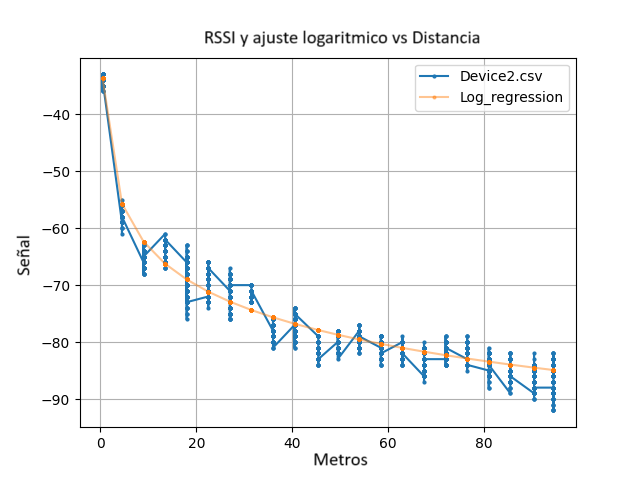
\includegraphics[width=0.8\textwidth]{Figuras/profiling/device2/device2-profiling.png}
	\captionsetup{margin=2cm}
	\caption[\acs{rssi} segregado por distancia de la medición vs regresión logarítmica, prueba de campo]{\acs{rssi} segregado por distancia de la medición vs regresión logarítmica, prueba de campo, con \acs{esp} en campo de deportes \acs{ungs}}.
	\label{fig:log-fit}
\end{figure}

La relación entre \acs{rssi} y la distancia se modela con la misma ecuación ya mencionada en la sección anterior. Con una pequeña diferencia en los signos para obtener números positivos.

\begin{equation}
    \text{RSSI} = -A - N \cdot \log(d)
\end{equation}

donde:

\begin{itemize}
    \item \(d\) representa la distancia entre el dispositivo emisor y el receptor.
    \item \(A\) es el valor de \acs{rssi} medido a una distancia de referencia de 1 metro. Que en vez de averiguar de manera experimental, procedemos a calcularlo usando las técnicas mencionadas.
    \item \(N\) es el coeficiente de pérdida de trayectoria, que refleja cómo la señal se atenúa con el incremento de la distancia.
\end{itemize}

Esta fórmula ajusta el \acs{rssi} observado a un modelo logarítmico, donde \(a\) y \(n\) son parámetros clave que se optimizan para ajustar el modelo a los datos recogidos.

Para convertir los valores de \acs{rssi} en estimaciones de distancia, se utiliza la inversión de la fórmula anterior:

\begin{equation}
    d = 10^{(-1 \cdot (\text{RSSI} + a) / n)}
\end{equation}

Para evaluar la bondad del ajuste, se calculó el residual como la norma euclidiana de la diferencia entre los valores observados y los predichos por el modelo. Este residual proporciona una medida cuantitativa de la discrepancia entre el modelo y los datos reales, sirviendo como indicador de la precisión del ajuste.

\begin{equation}
    \text{residual} = \lVert \text{RSSI observado} - \text{RSSI predicho} \rVert
\end{equation}

El valor de R, definido como $100 - \text{residual}$, ofrece un indicador para interpretar la calidad del ajuste; valores cercanos a 100 indican un ajuste muy preciso, mientras que valores más bajos sugieren una mayor discrepancia entre el modelo y los datos reales.

\subsection{Implementación}

Se implementaron scripts en \textit{Python} para realizar el ajuste logarítmico y el cálculo del residual, como el extracto que se puede ver en \ref{fig:log-fit-script} y cuyo código completo se encuentra en la sección \ref{herramientas_software}. Estos scripts permiten automatizar el proceso de ajuste y evaluación para diferentes conjuntos de datos, facilitando la experimentación y el análisis.

La figura \ref{fig:log-fit} muestra un ejemplo de gráfica resultante de aplicar dicho script, ilustrando cómo el modelo ajustado se alinea con las mediciones reales de \acs{rssi} segregadas por distancia.

\section{Filtrado de Kalman}
\begin{figure}[!htb]
	\centering
	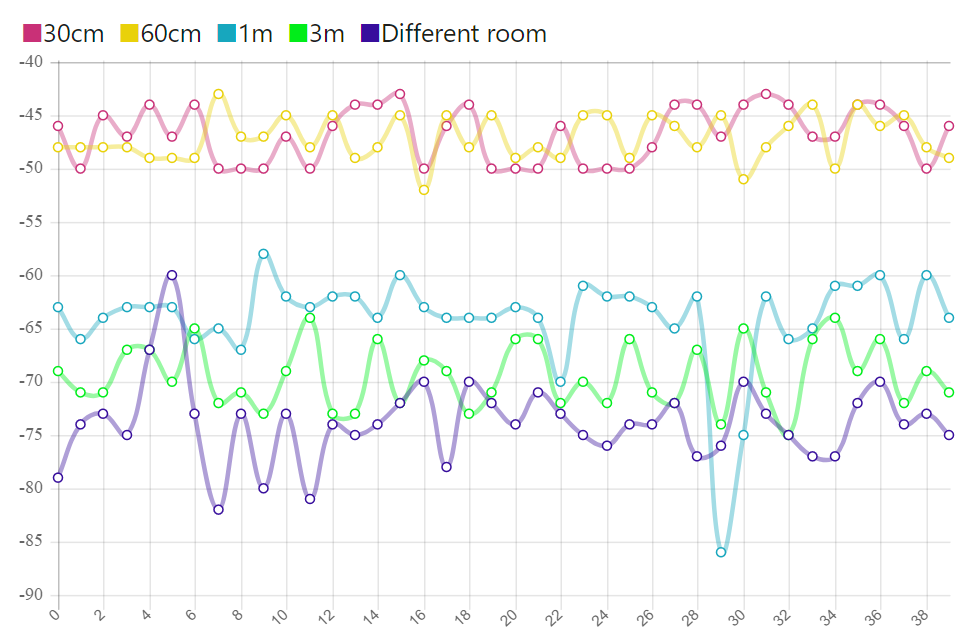
\includegraphics[width=0.8\textwidth]{Figuras/fig6.png}
	\captionsetup{margin=2cm}
	\caption[\acs{rssi} recibido a distintas distancias]{\acs{rssi} recibido a distintas distancias. (Kalman filters explained: Removing noise from \acs{rssi} signals. Wouter Bulten)}
	\label{fig:rssi-wouter}
\end{figure}

\begin{figure}[!htb]
	\centering
	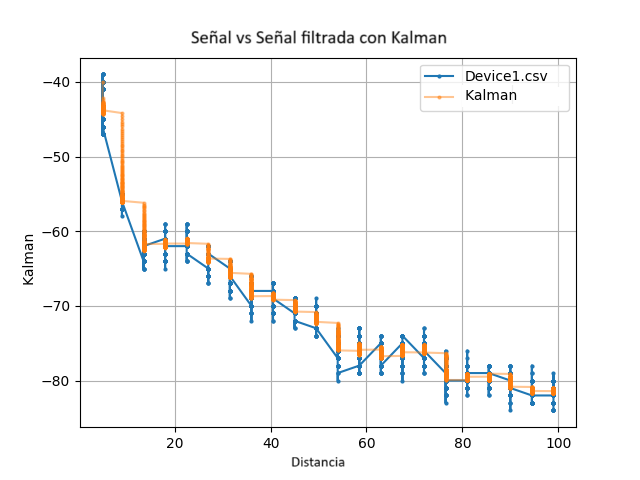
\includegraphics[width=0.8\textwidth]{Figuras/profiling/device1/Device1Kalman.png}
	\captionsetup{margin=2cm}
	\caption[Medicion de \acs{rssi} original y filtrada con Kalman, prueba de campo con \acs{esp} en campo de deportes \acs{ungs}]{Medicion de \acs{rssi} original y filtrada con Kalman, prueba de campo con \acs{esp} en campo de deportes \acs{ungs}}
	\label{fig:filtrado-kalman}
\end{figure}

El filtro Kalman es un algoritmo recursivo muy versátil que se utilizó en este trabajo  para estimar con más precisión la distancia a partir del \acs{rssi} recibido. Sobre todo en presencia de ruido e interferencia. Se decidió utilizar dicho filtro basándonos en el trabajo de Wouter Bulten et al. \cite{7471364} y del cual deriva un script en Python adaptado del original en Javascript por Sifan Ye \cite{SifanYe}. También se consultó como referencia otros trabajos similares como el de Tsanousa et al. \cite{tsanousa2021localization}.

Dicho filtro consiste en un estimador de estado que realiza una estimación de alguna variable no observada (en nuestro caso el \acs{rssi} real derivado de las mediciones observadas) basándose en mediciones ruidosas y teniendo en cuenta el historial de las mediciones anteriores. Un filtro de Kalman tradicional asume modelos lineales. Es decir, el paso del estado actual al siguiente debe ser una transformación lineal.

Se usará la identidad como matriz de transformación \(At\), y como no hay control sobre el movimiento, la matriz de control \(Bt\) se asume nula. Lo mismo ocurre con \(Vt\) el cual dejaremos en 0, ya que inicialmente asumiremos que no hay control sobre el objetivo. Finalmente, como el estado es modelado directamente, la matriz de observación \(Ct\) también se igualará a la identidad. Por otro lado, \(\epsilon_{t}\) y \(\theta_{t}\) representan el ruido de proceso y de medición, respectivamente.

 En consecuencia, el modelo de transición y observación se puede representar de la siguiente manera:

\[X_{t} = A_{t} * X_{t-1} + B_{t} + V_{t} + \epsilon_{t} = X_{t-1} + \epsilon_{t} \]

El paso predictivo lo calcularemos de la siguiente manera, donde R es el ruido de proceso que provendría del sistema en sí. Como sabemos que en este caso el ruido proviene de la medición y no del sistema, se asume un valor bajo (0.008). \(\sum\) se puede utilizar como indicador de la certeza de nuestra predicción. Entonces nos queda que la certeza en el paso \(t\) es igual a la certeza en el paso anterior más el ruido de proceso actual definido con la siguiente fórmula:

\[ \mu_{t}' = \mu_{t-1}  \]

\(\mu\) describe la predicción y x es el verdadero valor del estado. \(\mu’\) a diferencia de \(\mu\) indica que todavía no hemos incorporado la información sobre la medición. Es decir, es una predicción tentativa. Lo mismo aplica con Z y Z’.
\[\sum t' = \sum (t-1)' + R_{t} \]

La ganancia de Kalman, sera nuestra función de ponderación. Para ello usaremos Q como el ruido de medición; este indicador de ruido es más importante para este caso y deberá ser ajustado si se sabe que la interferencia puede deberse al movimiento del objetivo. Sin embargo, como inicialmente asumimos un modelo estático, entonces Q=3. La fórmula de la ganancia de Kalman entonces será la siguiente: 

\[K_{t} = K_{t}' ( \sum t' + Q_{t})^-1\]

Finalmente, el paso de actualización será de la siguiente manera:

\[ \mu_{t} = \mu_{t}' + K_{t}(Z_{t}-\mu_{t}')\]
\[ \sum t = \sum t' - (K_{t} \sum t')\]

En este último paso podemos notar que estamos calculando \(\mu_{t}’\), o sea la predicción final del sistema. Además, también hallamos el valor de \(\sum t\), nuestra certeza de predicción.
Este filtro logra adaptarse al entorno, decidiendo en base al histórico cuánta importancia darle a las nuevas mediciones por sobre las anteriores, ignorando el ruido a medida que este se agranda.

%\begin{figure}[th]

%	\centering

	%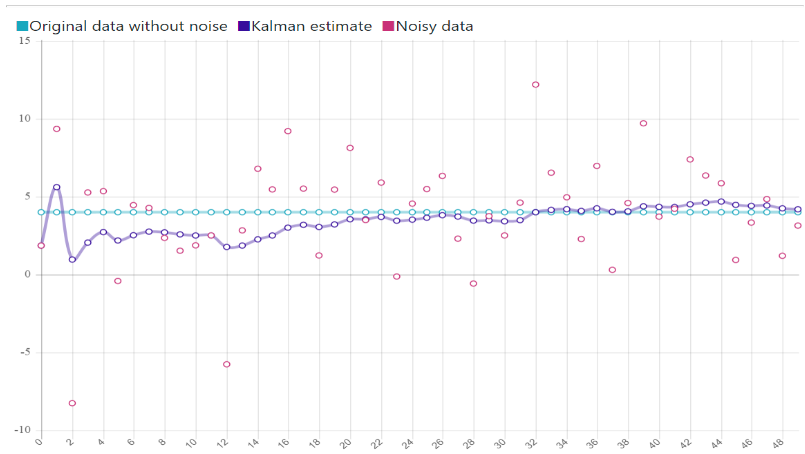
\includegraphics[width=0.8\textwidth]{Figuras/fig7.png}

%	\captionsetup{margin=2cm}

%	\caption[Datos con ruido vs kalman filter vs Datos verdaderos]{Datos con ruido vs Estimativo Kalman vs Datos originales. (Lightweight Javascript library for Noise filtering using Kalman filters)}

%	\label{fig:rssi-wouter-2}

%\end{figure}

Sin embargo, como este sistema no tiene manera de saber si el ruido de medición Q es producto del ambiente o producto de movimiento orgánico del objetivo, se podrá modificar luego el valor de \(V_{t}\) y \(B_{t}\) para indicar movimiento cuando lo haya y dejar de asumir así que se trata de un sistema estático. Se explorará esto más adelante en la sección de Multilateración.

En este trabajo usaremos las técnicas de filtrado \textit{Kalman} como paso previo de procesamiento antes de utilizar las capturas obtenidas por los nodos. De esta manera eliminamos gran parte de la interferencia momentánea o errores de medición y le damos más foco a la trayectoria de la señal en vez de los accidentes temporales que producen su fluctuación.

\section{Cuadrados Mínimos aplicado a Multilateración}

\label{sec:lsq}

Para resolver el problema de ubicar en 2D al objetivo solo teniendo las distancias estimadas hacia cada uno de los \textbf{Sniffers} es necesario algún algoritmo de localización. En este caso, como no se tiene el dato de la dirección en la que viene la señal, una triangulación no es posible. Para ello se usará en este trabajo el método de trilateración, cuya versión extendida a n nodos se llama multilateración, mediante el método de \textbf{Cuadrados mínimos}. Se evaluó durante el desarrollo de este trabajo la posibilidad de usar filtros de partículas como método de localización; sin embargo, dada su complejidad, queda para trabajo futuro analizar qué impacto de performance y precisión podría tener sobre experimentos simulados y reales.

La ecuación objetivo a resolver se plantea de la siguiente manera:

\begin{equation}
(x - x_0)^2 + (y - y_0)^2 = (dist_0 - r )^2
\end{equation}
\begin{equation}
\ldots
\end{equation}
\begin{equation}
(x - x_n)^2 + (y - y_n)^2 = (dist_n - r )^2
\end{equation}

Donde \textbf{Y}, \textbf{X} y \textbf{R} son las incógnitas a resolver, \textbf{Xi} e \textbf{Yi} son la posición del \textit{Sniffer} que capturó la señal, \textbf{dist\_i} es la distancia predecida en base al \acs{rssi} capturado, aplicando nuestra fórmula de Path Loss con el \textbf{A} y \textbf{N} hallados anteriormente. Se asume los mismos \textbf{A} y \textbf{N} para cada nodo; sin embargo, existen trabajos donde, durante la etapa \textit{offline}, es decir, cuando se calibra la señal, se usa un \textbf{A} y un \textbf{N} distinto por cada nodo e incluso uno distinto por cada orientación de nodo \cite{etter2019simulation}. A pesar de esto, se decidió optar por un modelo más simple, ya que en simulaciones dio buenos resultados.
\chapter{Experimento Simulado}
\label{Capitulo_3}
\label{ExperimentoSimulado}
Antes de plantear un experimento real, decidimos probar nuestro sistema en un caso experimental. Para eso, se decidió usar \acs{ns3} (\acl{ns3}). \acs{ns3} es un simulador de redes que permite no solo emular protocolos de enrutamiento como \acs{odv} (\acl{odv}) sino también aplicarle movilidad a los nodos y utilizar distintos modelos de \textit{Path Loss}.
Para este experimento simulado, se decidió configurar una red \textit{Ad Hoc} entre todos los nodos. Y se usó un modelo de propagación ideal: el \textbf{ns3::FriisPropagationLossModel}.
Uno de los nodos, nuestro \textbf{Objetivo}, se configuró como el nodo transmisor. Este emite mensajes constantemente de tipo \textit{broadcast} que, al estar conectados en una red \textit{ad hoc}, todos reciben.
Cada nodo tiene un script que, al recibir un mensaje de \textit{broadcast} del nodo \textbf{Objetivo}, guarda la ubicación real de este y el \textbf{RSSI} con el que se recibió el paquete.
Mientras esto ocurre, usando un modelo de movilidad, se le aplica un recorrido al nodo \textbf{Objetivo}. Mientras tanto, los otros nodos, que hacen las veces de \textit{Sniffer}, permanecen quietos durante todo el experimento. Al finalizar la simulación, se recopilan los datos en un archivo \textit{.csv} para luego ser analizados por herramientas propias.
\section{Perfilado}
\subsection{Implementación}
\begin{figure}[!htb]
\centering
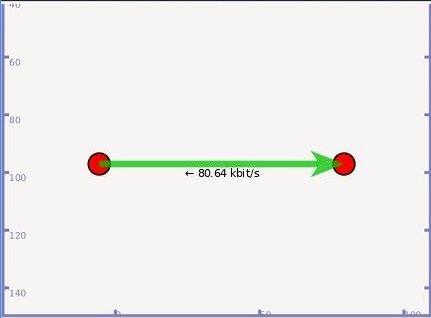
\includegraphics[width=0.5\textwidth]{Figuras/profiling/simulation/profiling_pyvis_going_away2.jpg}
\captionsetup{margin=2cm}
\caption[Visualización de la simulacion de NS3. El nodo objetivo se aleja del nodo Sniffer.]{Visualización de la simulación de \acs{ns3}. El nodo objetivo se aleja de uno de los nodos \textit{Sniffer}.}
\label{fig:simulated-ns3-profiling}
\end{figure}
En el caso del experimento de perfilado simulado, se utilizó un solo nodo \textit{Sniffer} que recibe paquetes de un nodo \textit{Objetivo} a medida que este se aleja. El resultado de la simulación es un archivo \textit{CSV} compuesto por filas (\textbf{distancia}, \textbf{rssi}). Finalmente, tomamos estos datos de \acs{rssi}, más los datos reales de distancia (calculados en la misma simulación) y realizamos un ajuste de curva hasta encontrar los valores de \textbf{N} y \textbf{A}. Estos nos servirán más adelante para predecir la distancia de dicho nodo en base a su \acs{rssi}.
El código para este experimento se encuentra en el siguiente archivo \href{https://github.com/agusalex/ns3-rssi-trilateration/blob/main/src/1DDistanceProfiling.cc}{\textbf{1DDistanceProfiling.cc}}.
Finalmente, se graficó la señal y la curva usando \textit{pyplot}.
\subsection{Experimento}
\begin{table}[!htb]
\centering
\begin{tabular}{|c|c|}
\hline
distance & rssi \\
\hline
10 & -52.55195 \\
11 & -54.77925 \\
12 & -56.68085 \\
13 & -58.339575 \\
14 & -59.810625 \\
15 & -61.132175 \\
16 & -62.33185 \\
17 & -63.43025 \\
18 & -64.443175 \\
19 & -65.383025 \\
20 & -66.2595 \\
21 & -67.080725 \\
22 & -67.85325 \\
23 & -68.5825 \\
24 & -69.273075 \\
25 & -69.928875 \\
\hline
\end{tabular}
\caption{Extracto de captura simulada de perfilado (capture.csv)}
\label{table:1}
\end{table}
Para poder saber la relación entre los \acs{rssi} recibidos y la distancia, es necesario perfilar nuestro dispositivo. Esto se debe a que distintos dispositivos \acs{wifi} con distinto hardware tienen distintas características de transmisión y recepción, por ejemplo, por la antena misma que este posee. Al perfilar, entonces sabremos con qué intensidad recibe la señal transmitida por el dispositivo móvil de prueba y cómo decae esa señal a medida que este se aleja. Esto tiene como objetivo final averiguar los valores de \textbf{N} y \textbf{A} para completar nuestra fórmula de conversión de \acs{rssi} a distancia.
El perfilado se realizó primero en un ambiente simulado para probar la eficacia de nuestros algoritmos y, finalmente, un experimento real.
En este experimento en particular en \acs{ns3}, se les aplicó a los nodos, dentro de una misma red \textbf{Ad-Hoc}, un modelo de movilidad donde un nodo \textbf{Sniffer} permanece quieto mientras que el otro, el nodo \textbf{Objetivo}, se aleja de este hasta \textbf{100} metros y su señal decae.
Después de llevar a cabo la simulación y recopilar los datos resultantes en un archivo .csv, procedimos con el análisis de los mismos. Los datos recogidos representaban la relación entre la intensidad de la señal \acs{rssi} y la distancia entre los nodos, que fue crucial para luego perfilar nuestro dispositivo utilizando \textbf{lmfit}.
\subsection{Conclusión}
En la Figura \ref{fig:profiling-result-sim}, se puede apreciar un decaimiento de la señal \acs{rssi} del nodo \textbf{Objetivo} conforme este se aleja del nodo \textbf{Sniffer}. Se observa un rango efectivo de menos de \textbf{51} metros, con pérdidas de señal muy frecuentes superados los \textbf{50} metros.
\begin{figure}[!htb]
\centering
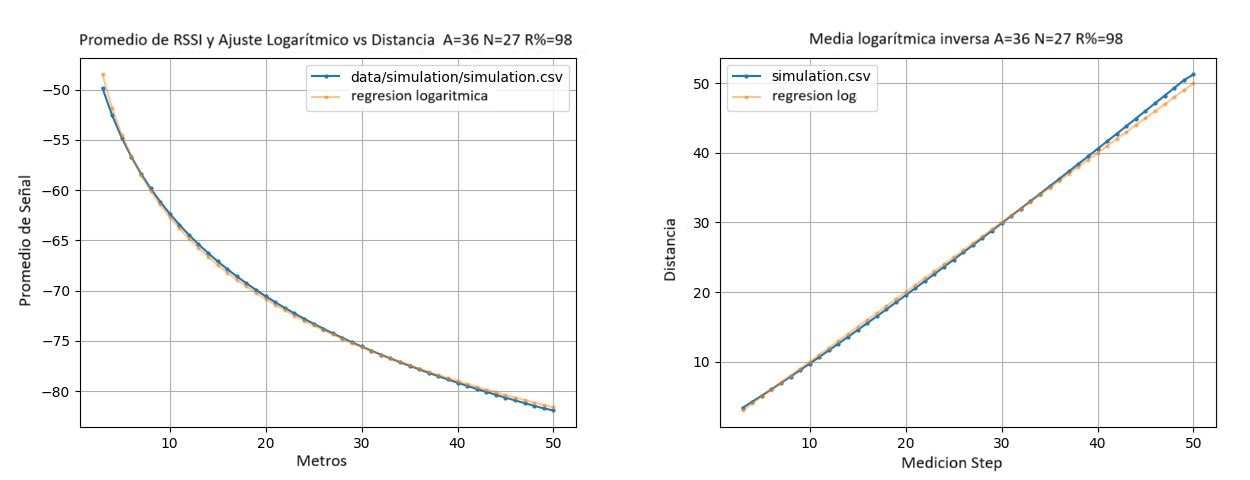
\includegraphics[width=0.99\textwidth]{Figuras/profiling/simulation/simulated-profiling-combo.jpg}
\captionsetup{margin=2cm}
\caption[ A la derecha, media de RSSI segregado por distancia de la medición vs regresión logarítmica, simulación usando NS3. A la izquierda, inversa al logaritmo de la distancia y distancia predicha en base a A y N calculados para la media del RSSI]{A la derecha, media de \acs{rssi} segregado por distancia de la medición vs. regresión logarítmica, simulación usando \acs{ns3}. A la izquierda, inversa al logaritmo de la distancia y distancia predicha en base a \textbf{A} y \textbf{N} calculados para la media del \acs{rssi}.}
\label{fig:profiling-result-sim}
\end{figure}
Se pudo observar una pequeña deriva entre la ubicación real y la predicha, esto se debe a que el \textit{fitting} de la curva simulada no es perfecto y tuvo un pequeño margen de error. Ese error depende de la distancia de la medición, ya que hay partes de la curva que se ajustan mejor que otras. En este caso, muy cerca del transmisor (menos de 1 metro) y al borde de la pérdida de transmisión (más de 45 metros) es donde más difieren, como se puede observar en la figura \ref{fig:profiling-result-sim}.
A pesar de ser un entorno simulado, estos resultados nos proporcionan una visión preliminar útil de cómo se comportaría nuestro sistema en la realidad, verificando que nuestros algoritmos funcionan y es posible ahora sí llevarlo a una prueba de campo. Los próximos pasos implicarán la realización de pruebas en entornos reales. Además, este experimento nos proporcionó valores de \textbf{N} y \textbf{A}, necesarios para nuestra fórmula de conversión de \acs{rssi} a distancia que se utilizarán luego en el experimento de multilateración simulado.
\section{Multilateración}
\subsection{Implementación}
Similar al experimento simulado de perfilado, se utilizó \acs{ns3}, esta vez con más nodos y haciendo un recorrido en dos dimensiones. Se utilizó el siguiente script para ejecutar la simulación \href{https://github.com/agusalex/ns3-rssi-trilateration/blob/main/src/2DTrilateration.cc}{\textbf{2DTrilateration.cc}}.
Además, para identificar inequívocamente una captura de un paquete emitido puntual, se utilizó \emph{millis} para segregar paquetes al momento de realizar la multilateración. De esta manera, si dos paquetes (dos entradas del archivo \textit{csv}) potencialmente distintos tienen el mismo valor en la columna \emph{millis}, se consideran el mismo paquete en un momento dado y se calculan en la misma ecuación de multilateración.
\begin{figure}[!htb]
\centering
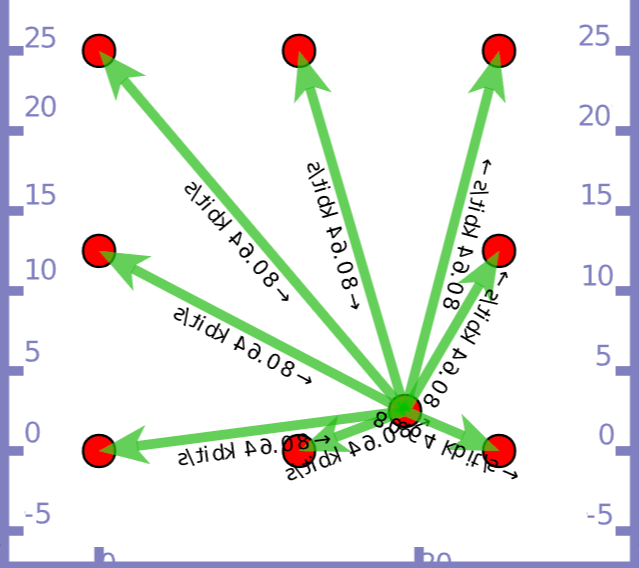
\includegraphics[width=0.5\textwidth]{Figuras/multilateration/simulated/multilateration-simulated-ns3.png}
\captionsetup{margin=2cm}
\caption[Visualización de la simulación de \acs{ns3}. El nodo objetivo realiza un recorrido mientras los otros ocho nodos Sniffer captan su señal.]{Visualización de la simulación de \acs{ns3}. El nodo objetivo realiza un recorrido mientras los otros ocho nodos \textit{Sniffer} captan su señal.}
\label{fig:simulated-ns3-mutilateration}
\end{figure}
\begin{table}[!htb]
\centering
\begin{tabular}{|c|c|c|c|c|c|c|c|}
\hline
millis & node & x & y & rssi & distance & target_x & target_y \\
\hline
9 & 2 & 12.5 & 0 & -63.5639 & 12.492 & 12.492 & 12.492 \\
9 & 4 & 25 & 12.5 & -63.5649 & 12.508 & 12.492 & 12.492 \\
9 & 5 & 0 & 12.5 & -63.5639 & 12.492 & 12.492 & 12.492 \\
9 & 7 & 12.5 & 25 & -63.5649 & 12.508 & 12.492 & 12.492 \\
9 & 1 & 0 & 0 & -68.0793 & 17.6664 & 12.492 & 12.492 \\
9 & 3 & 25 & 0 & -68.0799 & 17.6777 & 12.492 & 12.492 \\
9 & 6 & 0 & 25 & -68.0799 & 17.6777 & 12.492 & 12.492 \\
9 & 8 & 25 & 25 & -68.0804 & 17.689 & 12.492 & 12.492 \\
\hline
\end{tabular}
\caption{ Extracto de captura simulada que luego se usará como \textit{input} para multilateración. (Simulation.csv)}
\label{table:2}
\end{table}
El resultado de la ejecución es otro archivo \textit{csv} con las siguientes columnas: \textbf{millis}, \textbf{x}, \textbf{y}, \textbf{rssi}, \textbf{target\_x}, \textbf{target\_y}. \textbf{Millis} representa los milisegundos de la simulación, esto se usará luego para agrupar por ese criterio a la hora de hacer la multilateración. \textbf{X} e \textbf{Y} representan la ubicación del nodo que capturó el \textbf{rssi} de esa medición. Finalmente, \textbf{target\_x} y \textbf{target\_y} son la ubicación real del nodo \textbf{Objetivo} cuando la medición fue realizada, esto lo sabemos con certeza dado que el entorno es simulado.
Este archivo luego es procesado por nuestro algoritmo de multilateración, utilizando los valores de \textbf{A} y \textbf{N} hallados anteriormente para el perfilado simulado. Nuestro algoritmo de multilateración primero agrupa por paquetes que se hayan capturado al mismo momento, es decir, que los milisegundos (\textbf{Millis}) de la simulación sean los mismos. Luego solo se le aplicará multilateración y, de manera subsecuente, se agregarán al recorrido aquellos grupos de paquetes que al menos hayan sido capturados por 4 nodos o más. Esto se debe a que nuestro algoritmo de cuadrados mínimos necesita como mínimo al menos 4 nodos distintos para producir una predicción. Finalmente, se graficó el recorrido en 2d usando la biblioteca \textit{pyplot}.
\subsection{Experimento}
Inicialmente, se planteó un experimento con 4 nodos formando un cuadrado de 100x100 metros. Esto no produjo buenos resultados, ya que como el límite de recepción es alrededor de 50 metros, por momentos el nodo objetivo dejaba de estar al alcance de al menos 4 nodos y, entonces, la predicción fallaba. Esto se hacía evidente, produciendo recorridos que discrepaban enormemente del recorrido real. Al hacer más chico el cuadrado de 50x50 metros, la predicción se acerca mucho más a la realidad (Figura izquierda \ref{fig:ns3-multi-combined}). Finalmente, se diseñó un segundo recorrido de 25x25 metros, con 8 nodos (figura derecha \ref{fig:ns3-multi-combined}), mediante el cual se llegó al mejor resultado.
Usando \textbf{A = 36} y \textbf{N = 27} obtenidos durante el experimento de perfilado, se logró buena precisión a la hora de calcular el recorrido hecho por el nodo \textbf{Objetivo}.
\begin{figure}[!htb]
\centering
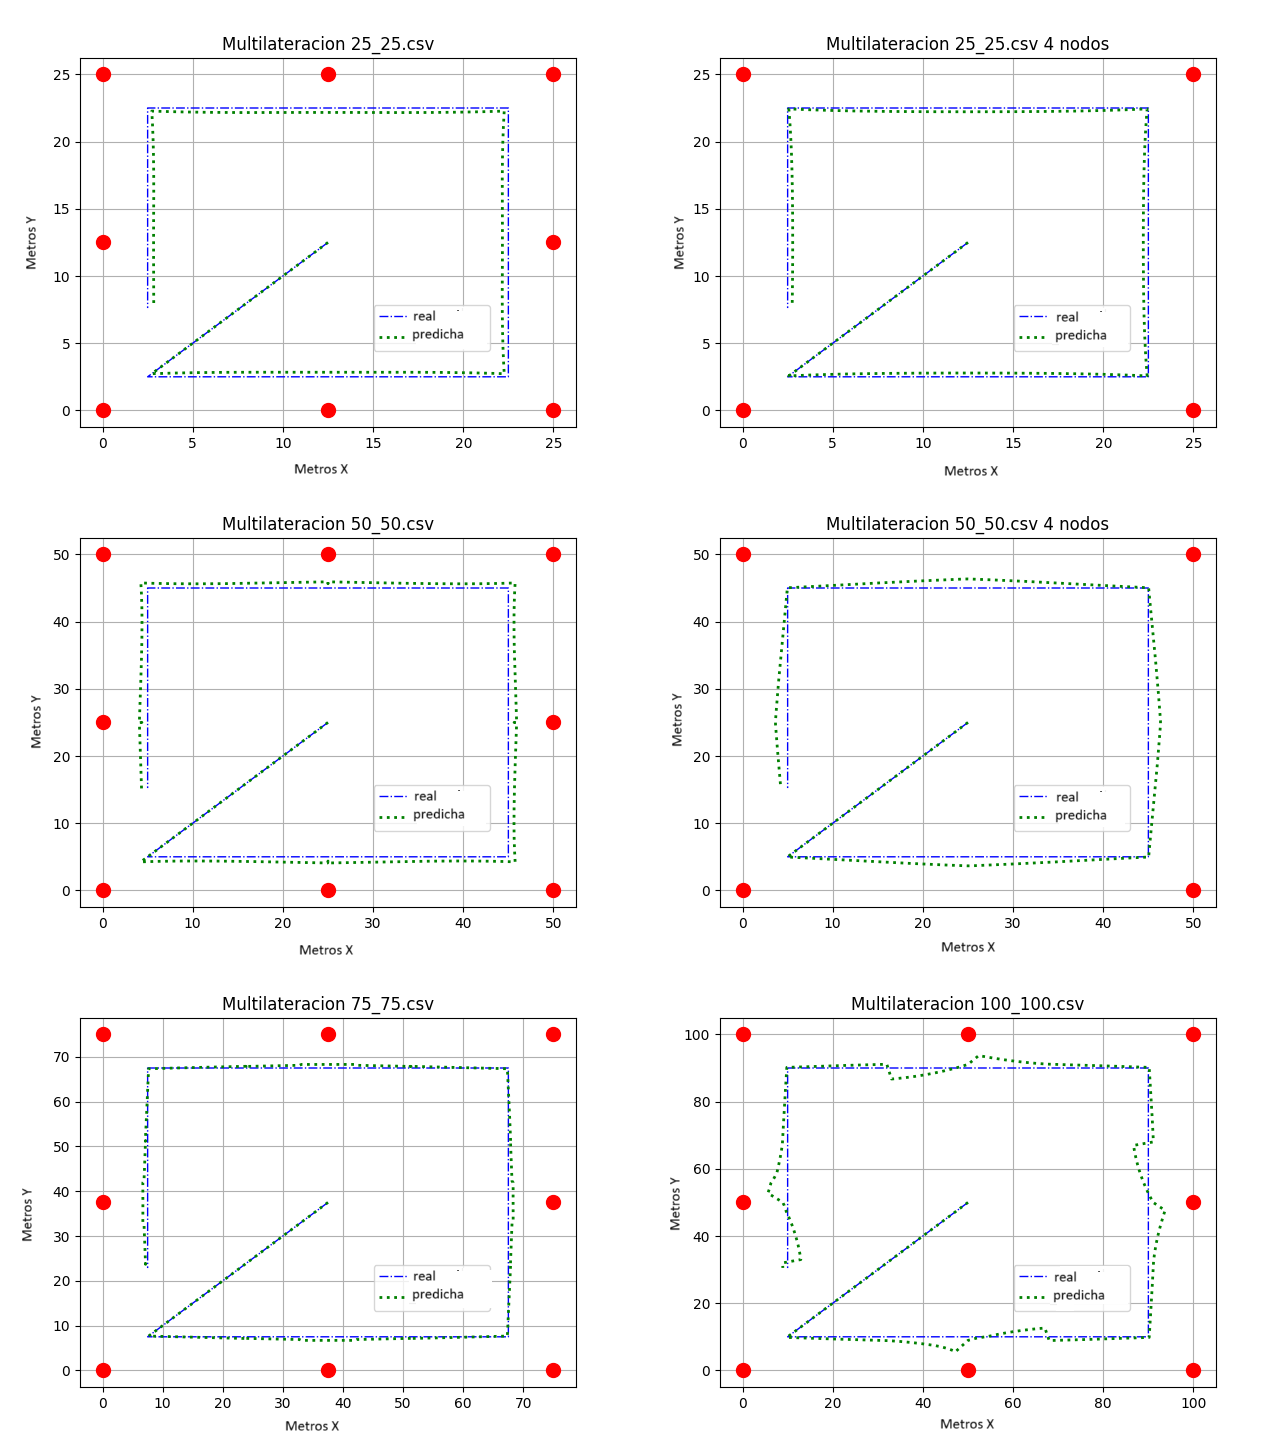
\includegraphics[width=0.99\textwidth]{Figuras/multilateration/simulated/many-sizes-and-node-count.png}
\captionsetup{margin=2cm}
\caption[Multilateración simulada]{Multilateración simulada. Se toman los datos de la simulación en \acs{ns3} más el \textbf{N} y \textbf{A} hallados y podemos conseguir ubicar a los nodos con los paquetes capturados. Se simularon distintos tamaños de grilla, desde 25x25 hasta 100x100. Cabe destacar que la precisión aumenta según la cantidad de nodos en el experimento y cuántos nodos reciben señal simultáneamente del objetivo. Esto último está relacionado al tamaño de grilla, ya que cuanto más lejos, menos nodos pueden recibir la señal.}
\label{fig:ns3-multi-combined}
\end{figure}
\section{Conclusión}
Se logró establecer un límite práctico en la cantidad mínima de nodos necesarios para determinar con precisión un recorrido durante una simulación, identificándose que con menos de cuatro nodos la predicción es inviable. Este requerimiento se explica por el uso de una ecuación tridimensional (involucrando las coordenadas \textit{x}, \textit{y} y el radio \textit{r}), a diferencia de los cálculos bidimensionales comúnmente usados cuando se realiza la técnica de trilateración, lo cual añade la precisión del radio a la medición pero exige un nodo adicional.
Este dato de precisión en la predicción (radio en metros de la predicción) es útil para poder descartar datos con mucho ruido. Adicionalmente, se observó que en escenarios con cuadrículas mayores a 50x50, la eficacia de la predicción disminuye progresivamente, atribuible a la reducción en el número de nodos receptores a medida que la distancia aumenta. Otro factor que incide en la pérdida de precisión es la creciente discrepancia entre las distancias predichas por el algoritmo durante la fase de perfilado y las distancias reales, particularmente al aproximarse a los 50 metros, punto en el que la capacidad de recepción del nodo transmisor se ve comprometida y la discrepancia aumenta, como se puede ver en la figura \ref{fig:profiling-result-sim}. Los experimentos de simulación, no obstante, arrojaron resultados prometedores, facilitando el desarrollo de técnicas y herramientas y permitiendo iterar rápidamente el proceso de desarrollo para encontrar soluciones en un entorno controlado. El perfilado proporcionó valores específicos para las variables \textbf{A} y \textbf{N}, cuya aplicación en experimentos de multilateración simulados confirmó la viabilidad del algoritmo. Esta fase de simulación culminó con buenos resultados, posibilitando avanzar hacia pruebas de campo por parte del equipo de investigación.
\chapter{Experimentos de campo}

\label{Capitulo_4}
\label{ExperimentoReal}
\section{Perfilado preliminar con \textbf{“\textit{steps}”}}
\subsection{Implementación}
\begin{figure}[!htb]
	\centering
	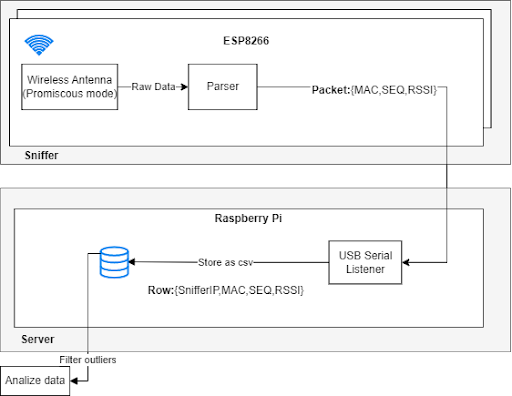
\includegraphics[width=0.7\textwidth]{Figuras/infraestructure/arduino-rpi.png}
	\captionsetup{margin=2cm}
	\caption[Flujo de datos en mediciones de perfilado]{Flujo de datos en mediciones de perfilado. El Arduino transfiere los datos mientras llegan directamente a la \acs{rpi} mediante \acs{usb}. Estos se agrupan por distancia (ingresada por el usuario) gracias al script de captura.}
	\label{fig:infra-diagram-arduino}
\end{figure}
\begin{figure}[!htb]
	\centering
	\includegraphics[width=0.8\textwidth]{Figuras/fieldwork/profiling-setup.png}
	\captionsetup{margin=2cm}
	\caption[Perfilado]{Experimento de campo de perfilado. Para que todos los dispositivos tengan sus antenas orientadas en el
mismo ángulo hacia la misma ubicación durante todo el experimento se utilizó
un soporte de metal con monturas hechas con impresora 3D.}
	\label{fig:arduino-profiling-setup}
\end{figure}

Antes de avanzar con los experimentos de campo hacia la etapa de multilateración, se quiso confirmar primero que la relación \acs{rssi} a distancia que informaban los \acs{esp} se acercaba a la realidad (es decir que se aproxime a lo que debería ser el ideal, o el modelo de \textit{Path Loss} antes visto). Similar a lo realizado en el experimento simulado pero con más nodos \textbf{Sniffer} para garantizar precisión.

Si bien se eligió utilizar una infraestructura \textit{wireless} más adelante como se describe en la sección \ref{sssec:num1}, primero se realizó un experimento preliminar cableado conectando tres \acs{esp} mediante \acs{usb} a una computadora \acl{rpi} para tomar múltiples muestras a una distancia conocida y poder poner un corte entre muestra y muestra a medida se recibíamos. De esta manera poder etiquetar múltiples muestras a 2 metros, a 5, a 10, etc.

Para recibir esta información se desarrolló un \href{https://github.com/agusalex/PacketSnifferServer}{script} que toma \textbf{M} muestras y luego se detiene a esperar a que el usuario le indique la nueva distancia en la que se realizará la próxima medición. De esta manera se obtiene \textbf{M} muestras agrupadas por la distancia, a esto le llamamos “\textit{step}”.


Además se decidió hacer el experimento de perfilado en un ambiente controlado (en el campo de deportes de la \acs{ungs} con muy poca interferencia en la banda 2.4 GHz). Se garantizó la precisión de los datos mediante la toma de 200 muestras por cada “\textit{step}” de medición. Y se realizaron 21 mediciones por cada dispositivo a 4.5 metros de distancia entre cada una. Dos de los dispositivos finalizaron el experimento, pero uno sufrió un desperfecto y dejó de recibir.
 
\begin{figure}[!htb]
	\centering
	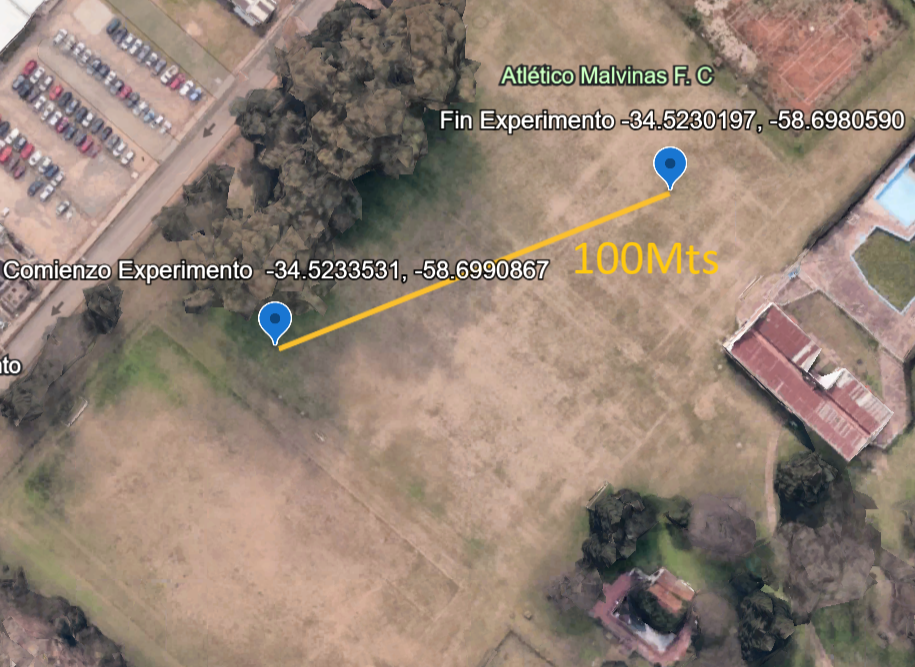
\includegraphics{Figuras/fieldwork/profiling.png}
	\captionsetup{margin=2cm}
	\caption[Perfilado]{Experimento de perfilado en el campo de deportes de la UNGS}
	\label{fig:arduino-profiling-setup}
\end{figure}
 Como transmisor se utilizó un dispositivo móvil en modo \acs{ap} para poder obtener una visión precisa del comportamiento de la señal.

Para procesar los datos de \acs{rssi}, primero se realizó un filtrado \textit{Kalman} de la captura entera por dispositivo, como se puede observar en la figura \ref{fig:filtrado-kalman}. Como último paso, calculamos la media por cada “\textit{step}” de distancia para filtrar las anomalías de los datos. Finalmente se ejecutó una regresión logarítmica usando cuadrados mínimos, el resultado nos da un \textbf{A} y un \textbf{N} que podría ser utilizado en el paso de multilateración.

\subsection{Experimento}
%\begin{figure}[!htb]
%	\centering
%	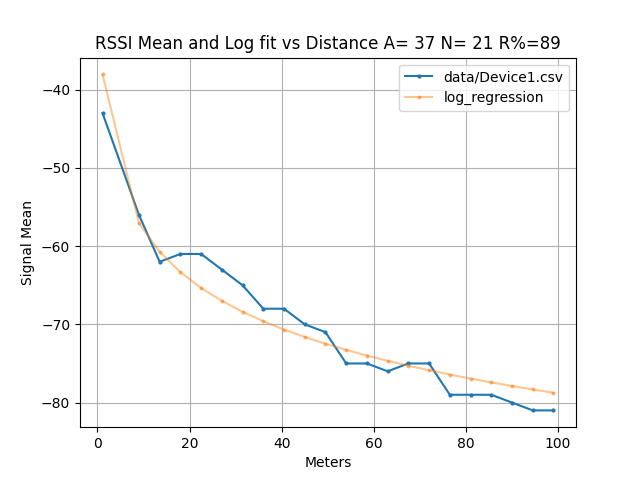
\includegraphics[width=0.8\textwidth]{Figuras/profiling/device1/device1_regression.png}
%	\captionsetup{margin=2cm}
%	\caption[Media de \acs{rssi} segregado por distancia de la medición vs regresión logarítmica, prueba de campo]{Media de \acs{rssi} segregado por distancia de la medición vs regresión logarítmica, prueba de campo con \textit{steps}”, con ESP8266 en campo de deportes UNGS. Se hallaron valores para \textbf{A=37}, \textbf{N=21} y \textbf{R(residual)=89\ }}
%	\label{fig:dev1-regression}
%\end{figure}

La figura \ref{fig:dev2-dev1-regression} muestra los resultados obtenidos de este experimento de campo. En el eje X se puede observar la distancia real desde el dispositivo \acs{esp} hasta el dispositivo móvil transmisor en metros, mientras que en el eje Y se representa el RSSI medido. Cada punto en el gráfico representa una medición individual del \acs{rssi} en una determinada distancia.



\subsection{Conclusión}

Puede observarse que a medida que la distancia aumenta, el \acs{rssi} se ajusta a una curva según lo predicho por el modelo, lo que se alinea con lo que esperaríamos de la pérdida de señal en función de la distancia en un entorno con mínima interferencia. Sin embargo, también se pueden identificar algunas variaciones y anomalías en los datos, posiblemente debido a factores ambientales no controlados o a variaciones inherentes en la recepción de la señal.
\begin{figure}
	\centering
	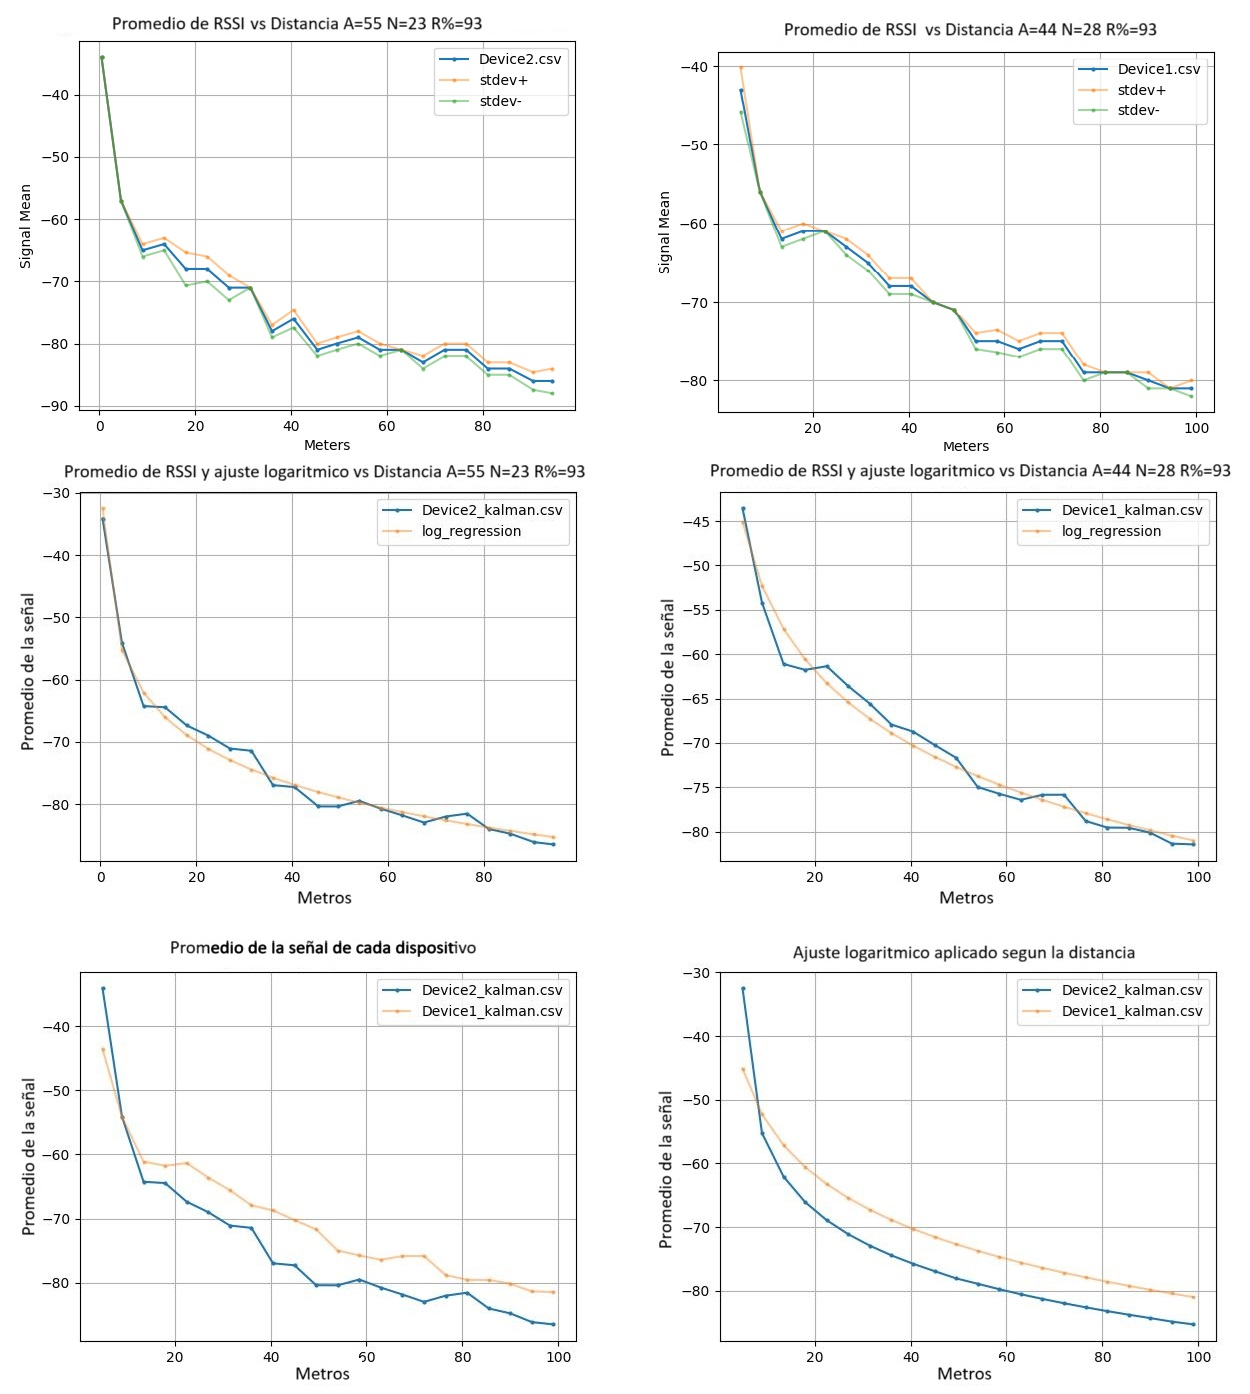
\includegraphics[width=1\textwidth]{Figuras/profiling/preliminar-experiment.jpg}
	\captionsetup{margin=2cm}
	\caption[Media de \acs{rssi} segregado por distancia de la medición vs regresión logarítmica, prueba de campo]{Media de \acs{rssi} segregado por distancia de la medición vs regresión logarítmica, prueba de campo con “\textit{steps}”, con ESP8266 en campo de deportes UNGS. Se hallaron valores del dispositivo 1 para \textbf{A=37}, \textbf{N=21} y \textbf{R(residual)=89}
    Para el dispositivo 2 \textbf{A=49}, \textbf{N=18} y \textbf{R(residual)=88}}
\label{fig:dev2-dev1-regression}
\end{figure}
Finalmente, realizamos una regresión logarítmica para obtener una representación ajustada de la relación entre la distancia y el \acs{rssi}. El resultado de esta regresión nos proporcionó los parámetros \textbf{A} y \textbf{N} para cada dispositivo, al igual que en el experimento simulado.




\section{Infraestructura de pruebas de campo \textit{wireless}} \label{sssec:num1}

\begin{figure}[!htb]
	\centering
	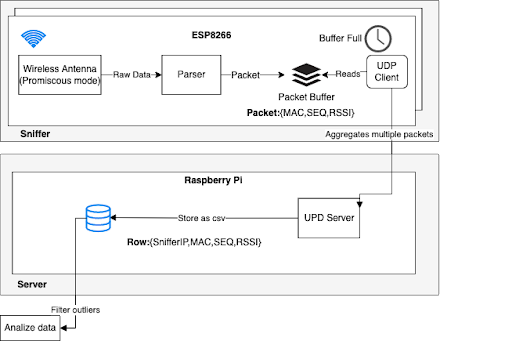
\includegraphics[width=0.8\textwidth]{Figuras/infraestructure/arduino-rpi-multi.png}
	\captionsetup{margin=2cm}
	\caption[Flujo de datos en mediciones de multilateración]{Flujo de datos en mediciones de multilateración. Los Arduinos recolectan los datos hasta agotar el espacio en memoria o llegar a un límite establecido. Finalmente descargan toda la información en una \acs{rpi} de manera inalámbrica.}
	\label{fig:infra-diagram-arduino}
\end{figure}

Se plantearon distintas alternativas de \textit{hardware} para poder cubrir el área más grande posible al menor costo. Se pensó en la utilización de \textit{routers} comerciales como los \textit{Ubiquiti} usando un software de código abierto como \textit{OpenWRT}, también la posibilidad de usar \acl{rpi} o similares e incluso microcontroladores con \acs{wifi} compatibles con Arduino como el \acs{esp} y el \acs{esp32}.

Cualquiera de estas soluciones trae consigo un problema ineludible: Los adaptadores \acs{wifi} hasta donde hemos podido investigar no pueden operar en modo promiscuo en simultáneo mientras que opera en otro modo, por ejemplo, en modo \acl{ap} o modo cliente mientras se encuentra en modo promiscuo. Se planteó la posibilidad de usar dispositivos que cuentan con dos adaptadores de \acs{wifi}, uno para capturar paquetes \acl{prq} y otro para evacuarlos hacia una base de datos centralizada para que luego puedan ser analizados pero no se encontró ninguno de bajo costo y de uso masivo.

Por esto fue elegida la alternativa de utilizar muchos dispositivos \acs{esp} como \textit{Sniffer} y un \textit{\acl{rpi} 3} en modo \textit{Access Point} para recibir los datos. Para facilitar las mediciones a modo de soporte aseguramos cada \textit{Sniffer} a un tubo de PVC con una base de cemento. Los \acs{esp} fueron adheridos con \textit{velcro} al tubo y se le agregó una batería de LI-ION conectada a los pines \acs{vin} y \acs{gnd} del dispositivo como se puede observar en la imagen \ref{fig:infra-diagram-arduino}.

El \acs{esp} fue programado utilizando Arduino y Platformio para el sensor y Python para el server que recibe los datos. Se configuró el dispositivo en modo promiscuo y se procedió a capturar paquetes y descomponer los \textit{Beacon Frames} en sus parámetros utilizando el \textit{SDK} del \acs{esp}. De dicho \textit{frame}, parte del 802.11, se extrae puntualmente el \acs{rssi}, \acs{mac} y el número de secuencia del paquete.

Se configuró el \acs{esp} para conectarse a una red Wi-Fi emitida por una \textit{\acl{rpi}} (configurada en modo \textit{AP} para facilitarnos la infraestructura de red) y enviar a la \acl{rpi} vía \acs{udp} los paquetes agregados de a grupos de \textbf{N} paquetes donde \textbf{N} es el máximo número que se podía enviar sin llenar el \textit{frame} de \acs{udp}. De esta manera optimizamos el tiempo de envío ya que múltiples nodos enviando a la vez de a un paquete pequeño por vez vía \acs{wifi} tendían a sobrecargar a la red y a la \acs{rpi} que necesita procesar y escribir los datos en una tarjeta SD.
La \textit{\acl{rpi}} contenía un script que recibe los datos \acs{udp} de cada nodo, y guarda en un solo archivo CSV la siguiente información: \textbf{ip\_sniffer}, \textbf{rssi}, \textbf{num\_secuencia}. Luego ese archivo se descarga manualmente conectándose por SSH a la \acs{rpi}.

El número de secuencia se emplea como un identificador único para cada paquete, permitiendo su agrupación durante la realización de experimentos de multilateración o perfilado, similar a cómo se agruparon los paquetes por milisegundos de captura en los experimentos simulados. Este método elimina la necesidad de mantener relojes sincronizados entre los nodos, como sería necesario si se usaran los milisegundos de captura como criterio de agrupación. Sincronizar relojes en un entorno de infraestructura \textit{wireless} representaría un desafío considerable que se decidió evitar.
De esta manera, al analizar un paquete, podemos identificarlo con certeza y comparar de manera inequívoca los \acs{rssi} recibidos y la diferencia entre estos para cada \textit{Sniffer}.

Finalmente, una vez capturadas suficientes tuplas de (\textbf{número\_secuencia}, \textbf{rssi}) descartando las que no sean de la \acs{mac} de nuestro \textit{Objetivo}, los dispositivos cortan la recepción antes de llenar la limitada memoria del dispositivo, este proceso suele durar 2 minutos aunque varía según la tasa de transmisión de paquetes del \textit{Objetivo}. Luego los \acs{esp} proceden a agregar las tuplas capturadas y enviarlas de a grupos mediante \acs{udp} hacia la \acs{rpi}. Esta última recopila los datos y les agrega la \acs{ip} de cada \textit{Sniffer} para poder identificar de dónde vino la información para luego ser procesada. Finalmente se persiste en un archivo CSV.

Como nodo \textit{Objetivo} se utilizó un teléfono celular en modo \acl{ap} para incrementar la tasa de transmisión de paquetes. De esta manera nos limitamos a capturar los paquetes de tipo \textit{Beacon Frame} que emite el teléfono usando su \acs{mac} como filtro. Consideramos que es un buen equivalente a una situación donde un transeúnte cuenta con un teléfono sin estar en modo \acl{ap} pero emitiendo \acl{prq}. Esto, con la salvedad de la Mac Address Randomization y la escasa frecuencia de emisión de los \acl{prq}, lo que no lo haría beneficioso para este experimento.

\section{Interferencias y Rango Usable para Multilateración con ESP8266}
\begin{figure}[!htb]
	\centering
	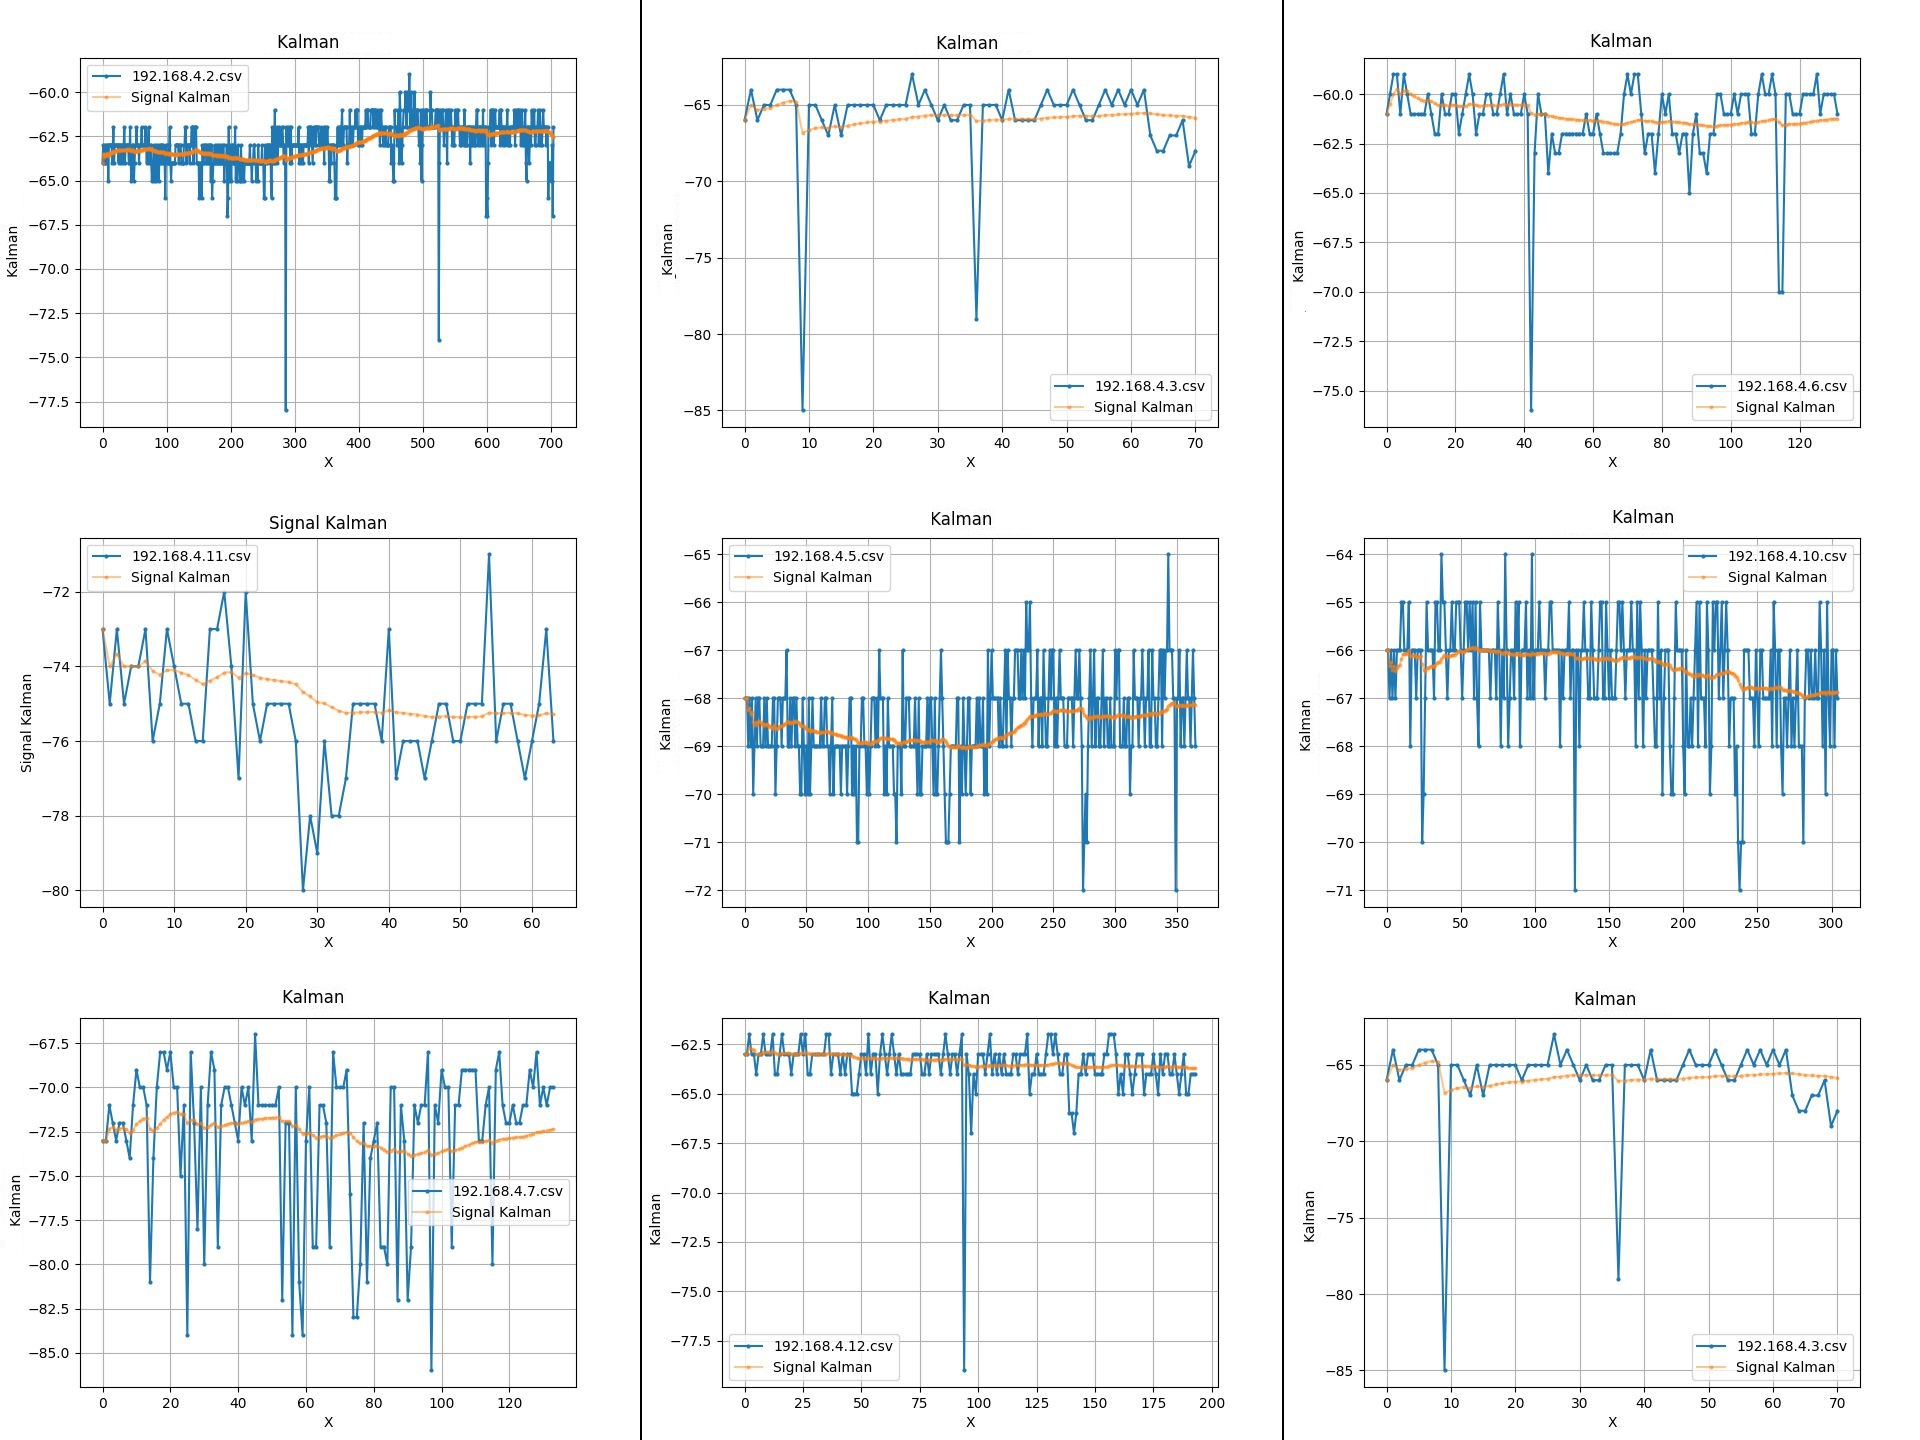
\includegraphics[width=0.95\textwidth]{Figuras/errores/estatico-medio.jpg}
	\captionsetup{margin=1cm}
	\caption[ Experimento estático]{ Experimento estático, misma disposición de nodos que el de multilateración. Se pueden observar grandes variaciones por interferencia del ambiente en el experimento sin movimiento. Los filtros de Kalman ayudan a mejorar esto.}
	\label{fig:errores-estatico}
\end{figure}
\subsection{Experimento estático}

 Utilizando la técnica de captura \textit{stepless} ya descrita se colocó un teléfono móvil a 15 metros de los nodos, los cuales se dispusieron en línea recta uno al lado del otro al igual que en el experimento de perfilado.
 Luego, sin mover el móvil, se procedió a capturar paquetes hasta completar la medición.
 Como se puede observar en la figura \ref{fig:errores-estatico} algunos nodos capturaron más datos que otros. Esto se debe a que durante la medición algunos nodos experimentaron fallos intermitentes en la alimentación, lo que provocó interrupciones en la recepción de señal. Durante la medición, algunos nodos experimentaron fallos intermitentes en la alimentación debido a un suministro de voltaje inadecuado. Esto ocurrió porque los nodos fueron alimentados directamente desde una batería de iones de litio con un voltaje nominal de 3.7V y un máximo de 4.2V, lo cual es insuficiente para el regulador AMS1117-3.3 integrado en la placa. Este regulador requiere un mínimo de 4.5V para operar correctamente; al no recibir un voltaje adecuado, la tensión de salida fluctuó por debajo de los 3.3V requeridos por el ESP8266, provocando estados inestables en su ejecución. Como resultado, algunos nodos dejaron de recibir paquetes al quedar en un estado de bloqueo (\textit{hang state}) o reiniciarse inesperadamente. Este problema afectó la consistencia de la captura de datos, generando discrepancias en la cantidad de paquetes registrados por cada nodo.

Otros experimentaron grandes interferencias, variando así por varios metros una potencial predicción de distancia.

 En todas las gráficas se puede ver cómo el filtro de Kalman ayuda a reducir el ruido y se adapta a los cambios en el perfil de recepción de la señal que persisten en el tiempo.
 Dicho filtro resultará una herramienta fundamental para mejorar la precisión en los experimentos subsiguientes.

\subsection{Precisión en el perfilado}


Luego de realizar varios experimentos de perfilado quedó en evidencia el problema que surge del modelo de \textit{Path Loss}: A medida que la distancia aumenta, la precisión baja considerablemente. Esto se puede observar en la figura \ref{fig:distance-error-range}, donde en la gráfica de la izquierda podemos observar cómo dada una posible interferencia temporal en la medición, la media de \acs{rssi} recibida a 12.5 metros es igual a la predicha por el ajuste logarítmico a 19 metros, en total un error de 6.5 metros. Lo que es más aún, la media de \acs{rssi} a 12.5 metros es igual a la media recibida a aproximadamente 25 metros, en total un error de 12.5 metros. Claramente, incluso a cortas distancias de menos de 20 metros se pueden ver distorsiones enormes en la distancia predicha. Continuando con este análisis, si consideramos la gráfica derecha en la misma figura, la cota inferior del desvío estándar (stdev-) a 27 metros es igual a la cota superior del desvío a 51 metros, en total, 24 metros de error entre ambos desvíos.

\begin{figure}[!htb]
	\centering
	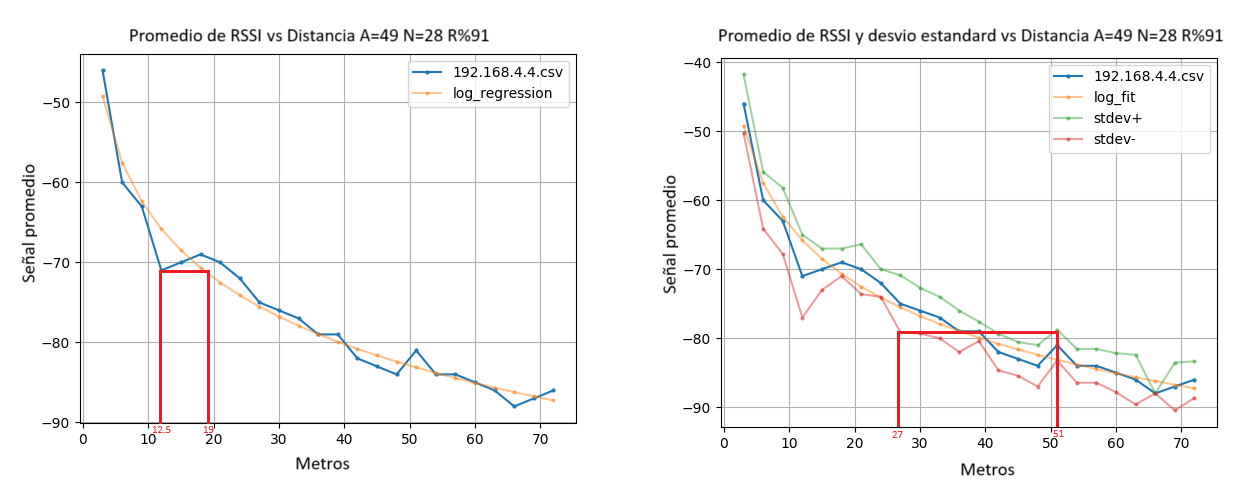
\includegraphics[width=0.95\textwidth]{Figuras/errores/4-raw-compilation-annotated.png}
	\captionsetup{margin=1cm}
	\caption[Variación de la distancia con \acs{rssi}]{Variaciones en la media y los desvíos estándar demuestran la poca precisión de estos dispositivos en distancias de más de 10 metros.}
	\label{fig:distance-error-range}
\end{figure}
\begin{figure}[!htb]
	\centering
	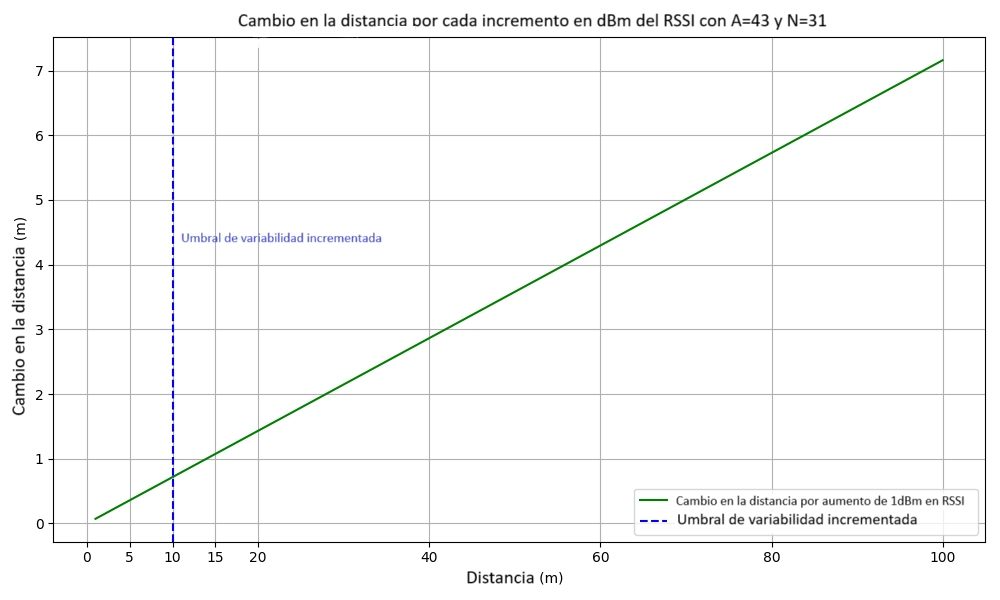
\includegraphics[width=0.95\textwidth]{Figuras/errores/distance_percentage_increase.png}
	\captionsetup{margin=1cm}
	\caption[Variación de la distancia con \acs{rssi}]{Variación de la distancia estimada por cada incremento de 1 dBm en \acs{rssi}, demostrando la precisión dentro de un rango de 10 metros y la creciente inexactitud más allá de este límite.}
	\label{fig:distance-percentage-increase}
\end{figure}

Por estos motivos se determinó que el rango usable efectivo de los dispositivos \acs{esp}, para experimentos de multilateración enfocados en identificar patrones de movimiento, es de hasta 10 metros. Incluso si se toma el modelo de \textit{Path Loss} sin interferencia como referencia, como podemos ver en la figura \ref{fig:distance-percentage-increase}, podemos observar que a partir de los 10 metros, por cada 1 dBm de variación en la intensidad de la señal \acs{rssi} se traducirá en cambios de aproximadamente 1 metro en la distancia estimada.

Este rango se ha demostrado adecuado para experimentos donde se buscaba determinar patrones de movimiento específicos, como patrones en forma de estrella o cuadrados, dentro de áreas confinadas. La elección de limitar las pruebas a una cuadrícula de 10x10 metros surgió tras experimentos multilaterales fallidos en áreas más extensas, como cuadrículas de 25x25 metros, donde el aumento de la imprecisión en las estimaciones de distancia comprometía la fiabilidad de los resultados.

Sin embargo, es importante destacar que el rango usable de 10 metros identificado en nuestra investigación es específico, primero, para el perfil de recepción de estos dispositivos y, segundo, puntualmente para la detección de patrones de movimiento detallados mediante multilateración. Para otros objetivos, como detección de presencia en áreas más amplias, el rango usable podría extenderse aún más. Y si consideramos el uso de antenas de mayor ganancia o la implementación de una mayor cantidad de dispositivos para cubrir un área mayor, este rango podría ser aún mejor.


\section{Perfilado sin \textbf{\textit{steps}}}

A pesar de los resultados prometedores obtenidos en los experimentos preliminares de perfilado, se hizo evidente que el perfilado es específico para cada sensor en un ambiente determinado. Esto se debe a que la curva de atenuación de la señal, que describe cómo disminuye la intensidad de la señal a medida que el transmisor se aleja, depende en gran medida del ruido ambiental del lugar donde se realice el experimento y de las características propias de cada dispositivo.

\begin{figure}[!htb]
    \centering
    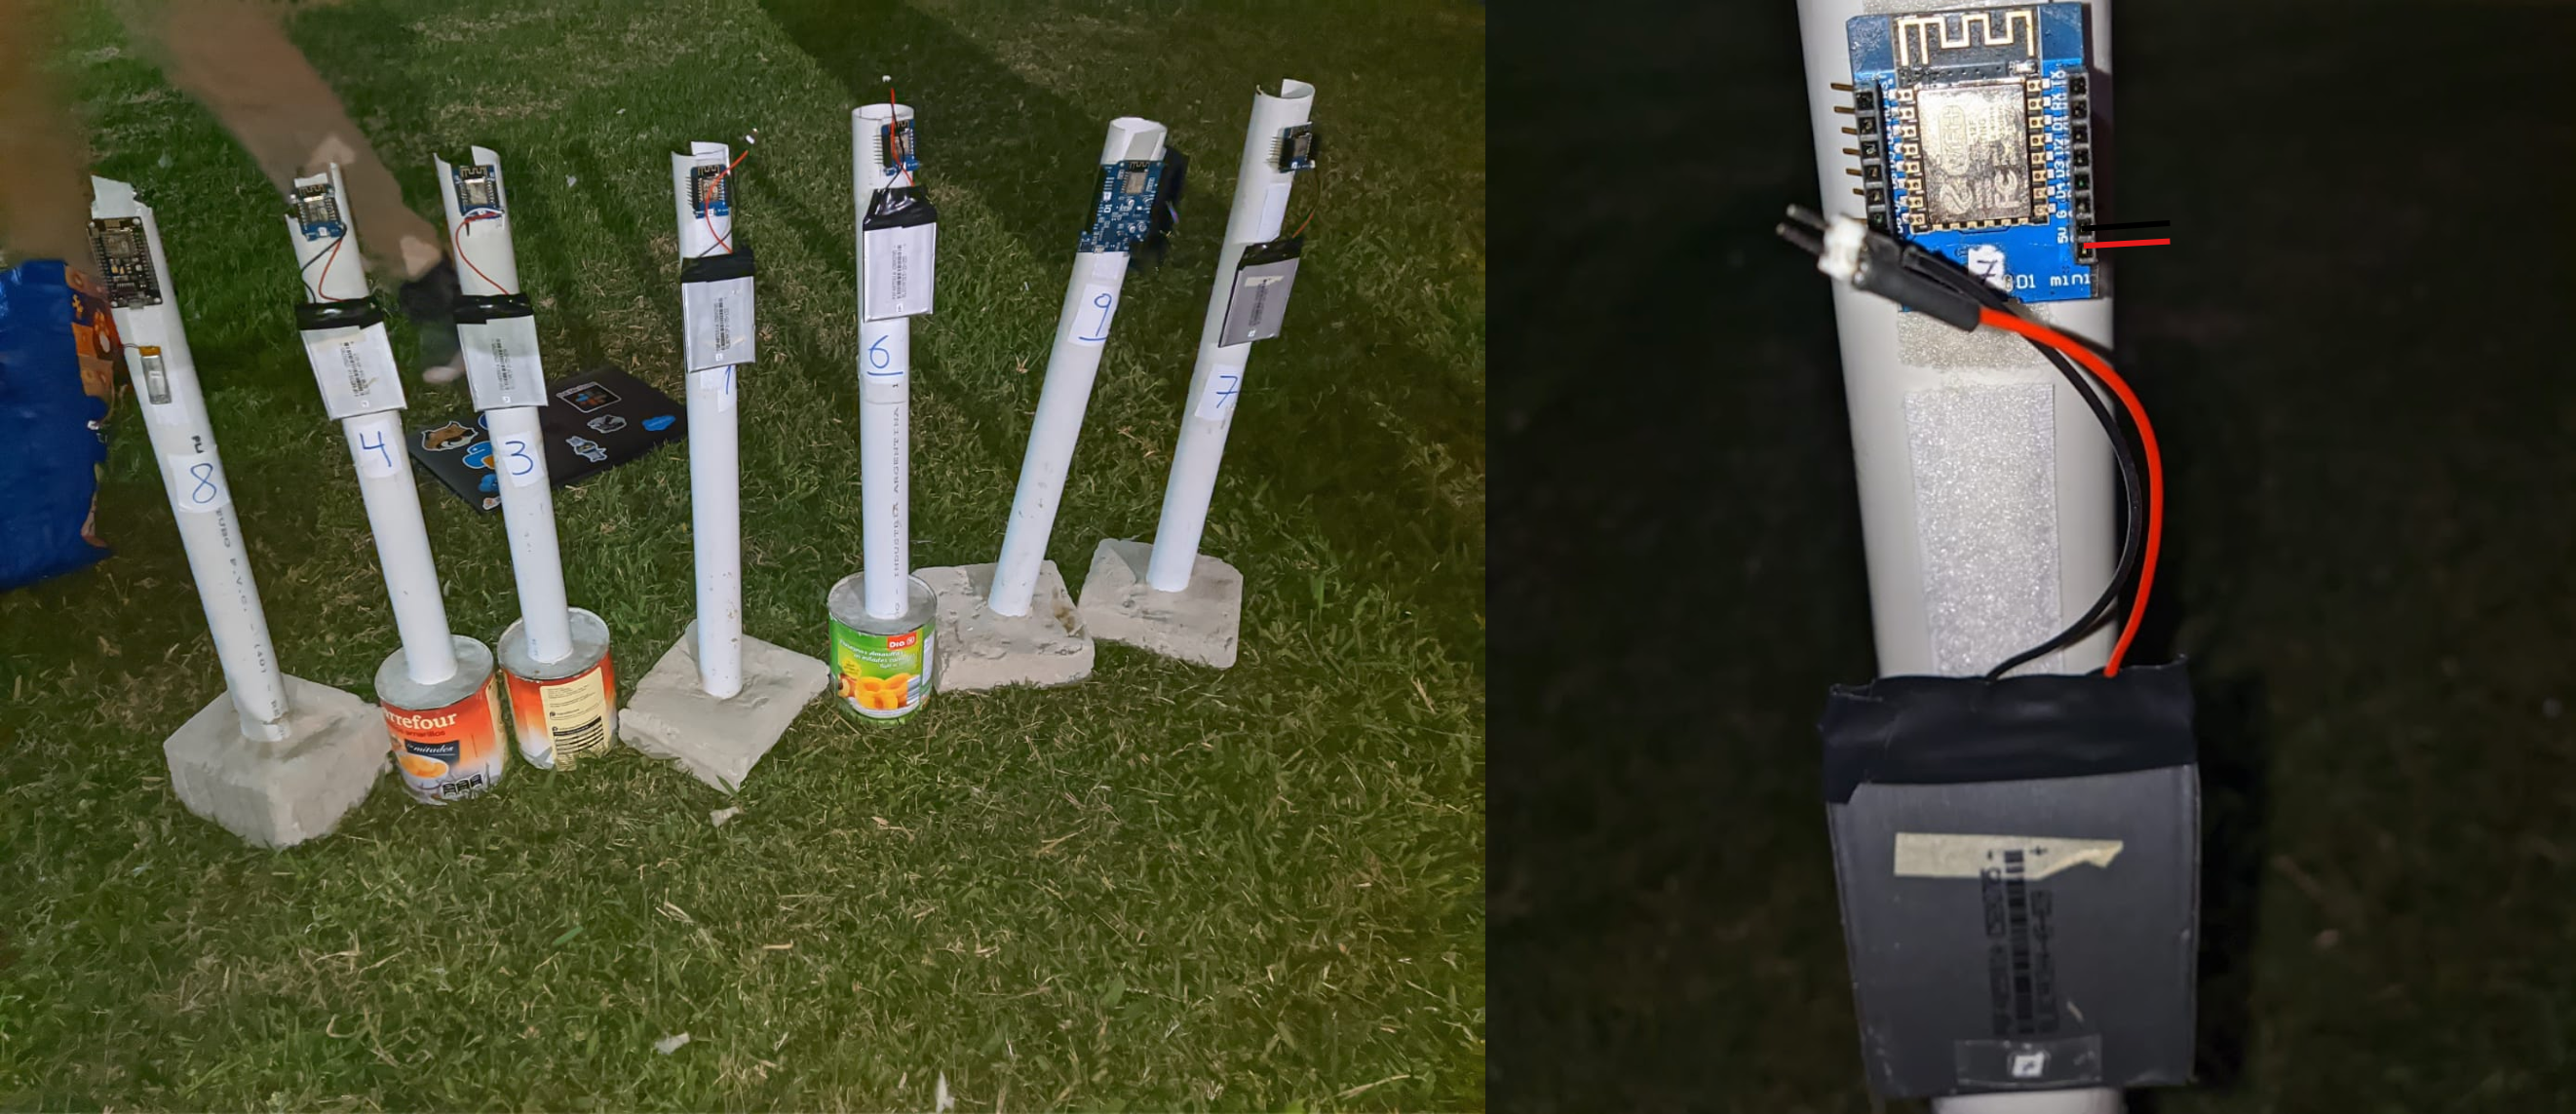
\includegraphics[width=0.8\textwidth]{Figuras/fieldwork/combined.png}
    \captionsetup{margin=2cm}
    \caption[Postes de Nodo Multilateración]{A la izquierda: Nodos \textit{Sniffer} construidos con PVC y una base de cemento. El ESP8266 fue adherido con velcro al tubo junto con una batería de LI-ION. A la derecha, un acercamiento a uno de los nodos notando donde se conectó el ESP8266 a la batería utilizando los terminales 5V y GND.}
    \label{fig:infra-diagram-arduino}
\end{figure}
Con el objetivo de evaluar la capacidad para predecir movimientos de un individuo en un ambiente urbano, y ante las limitaciones de acceso al campo de deportes de la \acs{ungs}, se optó por realizar experimentos en el campus de la \acs{ungs}, un lugar de alta concurrencia y con potencial interferencia de señal debido a la presencia de edificios. Del cual podíamos disponer en cualquier momento y así realizar más experimentos.

\begin{figure}[!htb]
    \centering
    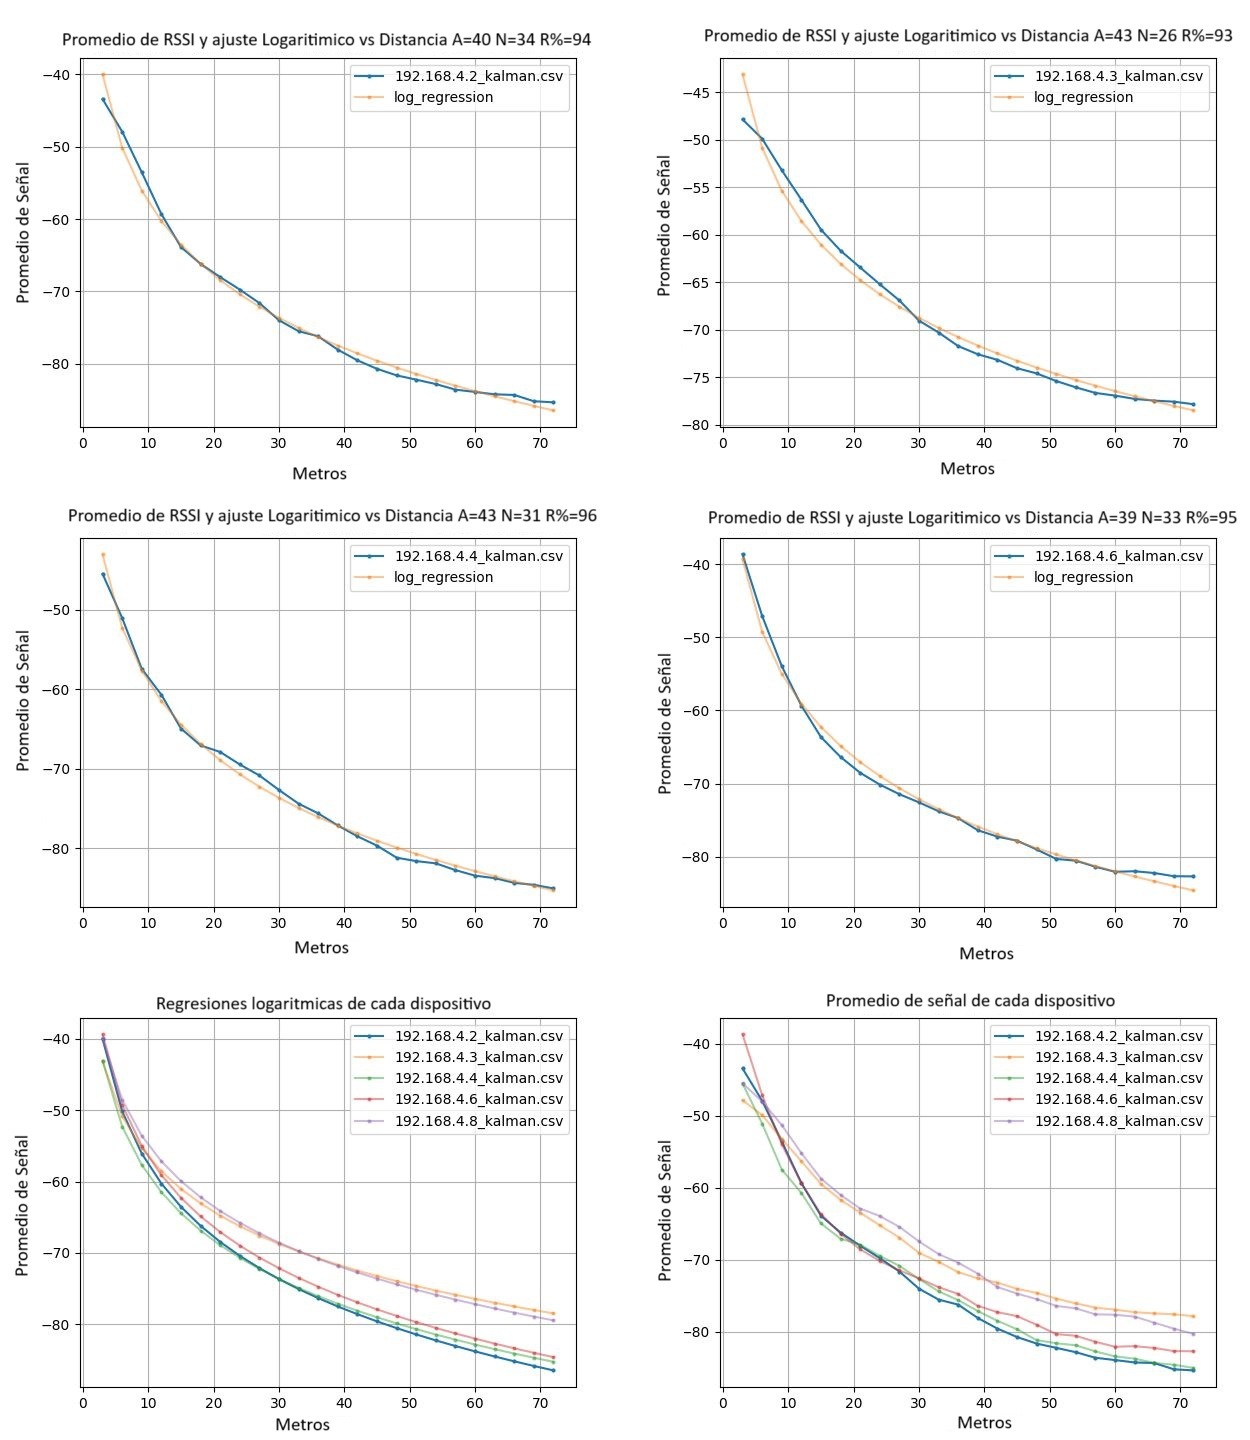
\includegraphics[width=0.95\textwidth]{Figuras/profiling/stepless.png}
    \captionsetup{margin=1cm}
    \caption[Stepless]{Resultados de perfilado \textit{stepless}.}
    \label{fig:stepless}
\end{figure}
Se decidió además probar el método de captura \textit{wireless} descrito en la sección \ref{sssec:num1} en un escenario de perfilado conocido antes de avanzar a la etapa de multilateración, con el fin de integrar todos los componentes de este trabajo. Este método no solo facilita la realización del experimento de perfilado, sino que también se asemeja más al escenario final de multilateración que se empleará posteriormente.

El término \textit{stepless} hace referencia a un enfoque de perfilado que no requiere de los pasos discretos predefinidos en términos de distancia conocida durante la captura de datos. En lugar de establecer intervalos fijos de distancia para la toma de mediciones, este método permite una captura continua a medida que el \textbf{Objetivo} se mueve a través del espacio. No obstante, para poder utilizar las ya mencionadas herramientas de perfilado, todavía se generan "pasos" virtuales basados en el tiempo y la secuencia de los paquetes capturados, lo que permite estimar la distancia recorrida. Estos pasos generados no corresponden a agrupaciones discretas con distancias conocidas, sino que son el resultado de una estimación que utiliza la secuencia de paquetes, la velocidad de movimiento y la frecuencia de transmisión del dispositivo móvil, facilitando así un análisis detallado sin la necesidad de mediciones de distancia fijas y conocidas previamente.

\subsection{Experimento}


A diferencia del experimento preliminar de perfilado realizado en el campo de deportes, este experimento se llevó a cabo en el campus de la UNGS.

Se dispusieron múltiples nodos en línea perpendicular al recorrido, formando una T con este, y se procedió a alejarse hasta alcanzar los 75 metros. Una vez completado el recorrido, se esperó a que los nodos finalizaran la captura y descarga de datos.

El método de captura \textit{wireless} empleado consiste en caminar a velocidad constante desde el punto donde se ubican los sensores, tomando nota del tiempo transcurrido hasta alcanzar una distancia determinada (por ejemplo, 30 metros en 30 segundos), mientras los sensores capturan los paquetes. Una vez finalizado el experimento, los datos se almacenan en la \acs{rpi}.

Dado que el dispositivo móvil utilizado (Samsung S20) emite paquetes cada 150 ms y conocemos el número de secuencia de cada paquete, es posible estimar la distancia a la que fue capturado y agruparlos en \textit{steps} discretos de distancia. Aunque se pierde precisión en la distancia exacta de captura, este agrupamiento y el cálculo del promedio mitigan el potencial error.

\subsection{Conclusiones}

El perfilado sin \textit{steps} permitió realizar experimentos de manera más rápida, facilitando la obtención de los valores de \(N\) y \(A\) en diferentes ambientes y para múltiples nodos simultáneamente, sin necesidad de conexión por cable o de tomar notas manuales sobre las distancias, reduciendo el tiempo de medición de 1 hora a 15 minutos. Además, se posiciona como una opción ideal para el despliegue rápido de nodos en un nuevo ambiente. Como se muestra en la figura \ref{fig:stepless}, se logró determinar los valores de \(N\) y \(A\) para cada sensor.

No obstante, algunos sensores presentaron interferencias significativas o su recepción se detuvo abruptamente, un problema recurrente a lo largo de este trabajo. La variabilidad observada en un experimento estático sin movimiento sugiere posibles defectos en los nodos o interferencias en el área de experimentación que afectaron a algunos nodos más que a otros, como se ilustra en la figura \ref{fig:errores-estatico-medio}.


\section{Multilateración}

\begin{figure}[!htb]
    \centering
    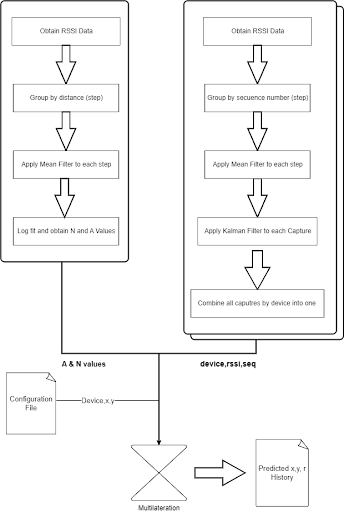
\includegraphics[width=0.6\textwidth]{Figuras/infraestructure/infra-diagram.png}
    \captionsetup{margin=2cm}
    \caption[Flujo de datos]{Flujo de datos en el experimento de multilateración.}
    \label{fig:infra-diagram}
\end{figure}
\begin{figure}[!htb]
	\centering
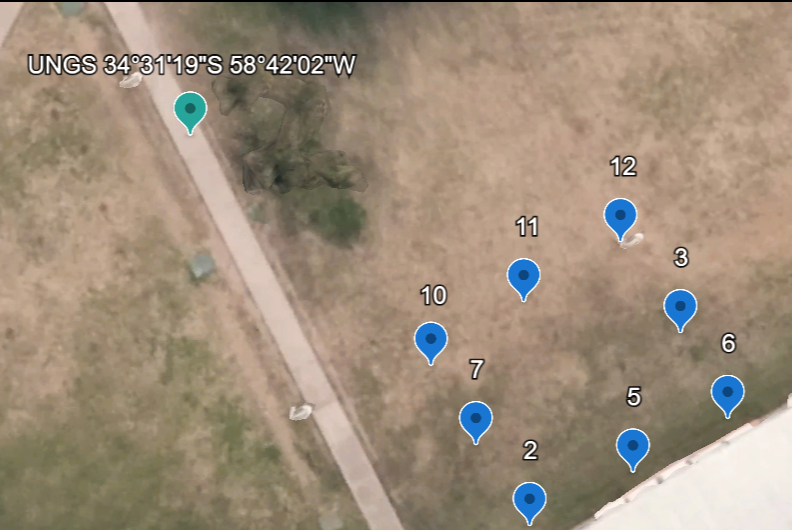
\includegraphics{Figuras/fieldwork/trilateration.png}
	\captionsetup{margin=2cm}
	\caption[Perfilado]{Experimento de perfilado en el campus de la UNGS}
	\label{fig:arduino-profiling-setup}
\end{figure}
\subsection{Infraestructura}

De manera similar al experimento de perfilado, se implementó una red de nodos \textbf{Sniffer} en el campus de la \acs{ungs}, siguiendo un esquema predeterminado. En este caso, se colocaron ocho nodos formando un cuadrado de 10 x 10 metros. Estos nodos se dedicaron a monitorear las señales Wi-Fi, capturando la intensidad de la señal \acs{rssi} emitida por el nodo \textbf{Objetivo}, que se desplazaba siguiendo una ruta preestablecida dentro del alcance de los nodos \textbf{Sniffer}. Durante el experimento, el nodo \textbf{Objetivo} mantuvo una velocidad constante.

Los nodos \textbf{Sniffer} registraron la \acs{rssi} de las señales emitidas por el nodo \textbf{Objetivo}, junto con el número de secuencia de cada señal, transmitiendo estos datos a una \acl{rpi} mediante Wi-Fi, una vez completado el experimento y llenados sus buffers para el posterior análisis de los datos.

Con los valores de \textbf{A} y \textbf{N} derivados de los experimentos de perfilado previos y utilizando la fórmula que convierte el valor de \acs{rssi} en distancia, se estimó la separación entre cada nodo \textbf{Sniffer} y el nodo \textbf{Objetivo} para cada paquete con el mismo número de secuencia. Se realizaron un mínimo de cinco mediciones de distancia con distintos nodos para cada punto en el tiempo para garantizar una mayor precisión.

Si bien durante la etapa de perfilado, se calculó un \textbf{A} y un \textbf{N} distintos para cada nodo. Tal como se discutirá más adelante, las interferencias fueron un factor muy importante durante las pruebas en el campus de la \acs{ungs}. Muchos nodos arrojaron valores muy distintos simplemente por los grandes cambios en la señal, incluso estando quietos, como se aprecia más adelante en la figura \ref{fig:errores-estatico}. Por este motivo, se eligieron los valores de \textbf{A} y de \textbf{N} del experimento de perfilado que mejor ajuste tuvo, es decir que tuvo menor residual.
En este caso \textbf{A=43} y \textbf{N=31}.

\begin{figure}[!htb]
\centering
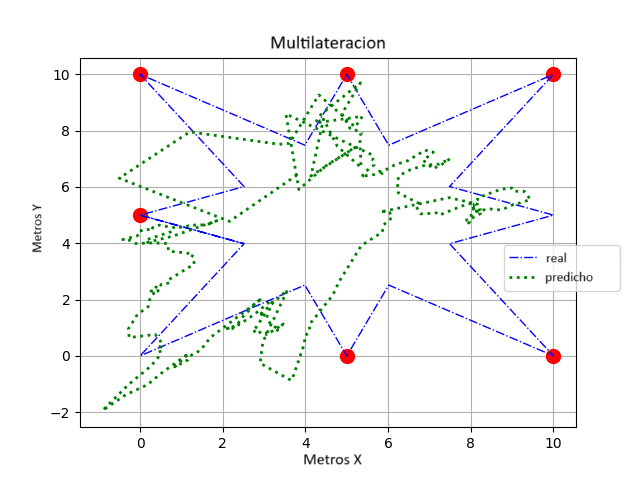
\includegraphics[width=0.8\textwidth]{Figuras/multilateration/multilateration_star.png}
\captionsetup{margin=2cm}
\caption[Configuración de la multilateración en Tiempo Real]{Configuración del experimento de multilateración en tiempo real en el campo de deportes de la \acs{ungs}.}
\label{fig:real-multilateration}
\end{figure}

\begin{figure}[!htb]
\centering
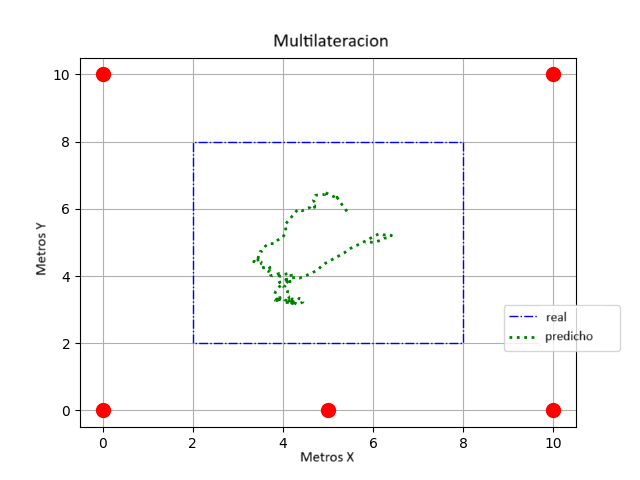
\includegraphics[width=0.8\textwidth]{Figuras/multilateration/multilateration_square.png}
\captionsetup{margin=2cm}
\caption[Resultados de la multilateración en Tiempo Real]{Resultados de la multilateración en tiempo real, mostrando la trayectoria estimada del nodo \textbf{Objetivo} en comparación con su trayectoria real.}
\label{fig:real-multilateration-results}
\end{figure}


\subsection{Experimento}

Se llevaron a cabo múltiples recorridos en distintas ejecuciones de este experimento. Si bien durante el experimento se utilizaron 8 nodos, en la figura \ref{fig:real-multilateration} solo se representaron con círculos rojos 6 nodos. En la figura \ref{fig:real-multilateration-results} se puede ver que solo hay representados 5 nodos. Esto se debe a que algunos nodos presentaron altas interferencias y sus datos fueron descartados. También se debe a que algunos nodos no recibieron señal parcial o totalmente en algunos o todos los experimentos. Estos fenómenos serán explicados en más detalle en el capítulo \ref{Cap_Errores}.
La multilateración se llevó a cabo comparando las posiciones estimadas del nodo \textbf{Objetivo} con su trayectoria real, con el fin de evaluar la precisión de este método. Aunque los resultados mostraron cierto nivel de error en la estimación de la ubicación, estos se discutirán en detalle en la sección siguiente.


Las estimaciones de la ubicación obtenidas mediante la multilateración, representadas en las figuras \ref{fig:real-multilateration} y \ref{fig:real-multilateration-results}, se compararon con la trayectoria real del nodo \textbf{Objetivo} para evaluar la precisión del método. En los gráficos, los nodos \textbf{Sniffer} están ubicados en posiciones fijas, mientras que el nodo \textbf{Objetivo} sigue una ruta predeterminada.

Cada punto en los gráficos simboliza una estimación de la posición del nodo \textbf{Objetivo}, calculada a partir de las mediciones de \acs{rssi} recogidas por varios nodos \textbf{Sniffer}, el número de secuencia de los paquetes, y los parámetros \textbf{A} y \textbf{N} obtenidos de los experimentos de perfilado.

La línea azul ilustra la trayectoria real seguida por el nodo \textbf{Objetivo}, mientras que la línea verde muestra las estimaciones de su posición según la multilateración. Se puede observar que las estimaciones recrean levemente la trayectoria original, aunque presentan grandes deformaciones.


\subsection{Conclusión}

A pesar de las discrepancias y deformaciones observadas en las estimaciones de la ubicación del nodo \textbf{Objetivo}, el recorrido estimado mantiene cierta semejanza con la trayectoria original. Esto indica que, aunque existen errores significativos en la precisión de la localización, el enfoque de multilateración empleado logra capturar la esencia del movimiento del nodo \textbf{Objetivo} dentro del área de cobertura de los nodos \textbf{Sniffer}. Sin embargo, se identificaron zonas donde las estimaciones se alejaban significativamente de la trayectoria real, atribuibles a diversos factores como la interferencia inalámbrica, movimientos no intencionados del nodo \textbf{Objetivo}, y errores en la medición de \acs{rssi}.

Dentro de los resultados obtenidos, las discrepancias constantes en las estimaciones de ubicación, manifestadas como desplazamientos constantes o rotaciones en el gráfico, pueden deberse a múltiples factores relacionados con el entorno y la metodología de medición. Un desplazamiento constante en las estimaciones indica un sesgo sistemático en la medición del \acs{rssi}, posiblemente a causa de diferencias en la ganancia de las antenas de los nodos \textbf{Sniffer} o que la antena del nodo \textbf{Objetivo} no fuera precisamente omnidireccional (como no suelen serlo en teléfonos móviles).

Por otro lado, las rotaciones observadas en la predicción del recorrido, podrían deberse a personas en el camino de la señal o errores en la ubicación de los nodos, por ejemplo, un velcro flojo y un nodo que apunta ligeramente hacia un lado o al otro. Factores adicionales, como la reflexión de señales en superficies cercanas o la difracción a través de obstáculos también pueden contribuir a los errores y deformaciones registrados.
\chapter{Discusiones}
\label{Cap_Errores}
\label{Capitulo_5}

Los experimentos realizados, tanto en entornos simulados como reales, han mostrado resultados alentadores en la estimación de ubicación, mostrando resultados prometedores en la estimación de ubicación. Al mismo tiempo, se han detectado ciertos errores y limitaciones que afectan la precisión del sistema. En este capítulo analizaremos en detalle los errores identificados y propondremos mejoras que permitan optimizar aún más el desempeño de un sistema similar.


\section{Análisis de Errores y Mejoras}

\subsection{Interferencia Ambiental y Variabilidad de la Señal}

Uno de los principales desafíos encontrados durante los experimentos fue la interferencia ambiental, que afecta significativamente la calidad y la consistencia de las señales \acs{wifi}. Como se muestra en la Figura \ref{fig:errores-estatico}, las variaciones en la intensidad de la señal \acs{rssi} debido a la interferencia del ambiente pueden introducir errores significativos en la estimación de la distancia y, por ende, en la localización del dispositivo.

Otro impedimento fue la inconsistencia en la recepción de paquetes, atribuible a inestabilidades en el suministro de energía de los dispositivos utilizados. Como se puede ver también en la Figura \ref{fig:errores-estatico}, se observó una marcada diferencia en el número de muestras recibidas: mientras algunos dispositivos capturaron hasta 700 muestras, otros apenas 70. Dado que no hubo movimiento en el experimento, estas discrepancias sugieren que, además de la interferencia ambiental, la variabilidad en la alimentación al usar batería de \textit{LI-ION} sin adaptar el voltaje a 5V continuo pudo haber afectado el desempeño, generando fallos a nivel de hardware.

\textbf{Se propone como trabajo futuro:}
Primero revisar la consistencia en la recepción mejorando la alimentación del hardware agregándole un módulo \textit{Step-Up} de 3V-4V a 5V. Para mitigar el impacto de la interferencia ambiental, se recomienda implementar algoritmos de filtrado más avanzados, como filtros de partículas o técnicas de aprendizaje automático, que puedan identificar y compensar las fluctuaciones anómalas en la intensidad de la señal en tiempo real. Además, el uso de modelos de propagación de señales más complejos que tengan en cuenta las características específicas del entorno urbano puede ayudar a mejorar la precisión de las estimaciones.

\subsection{Desafíos en la Multilateración y la Estimación de Distancias}

La multilateración, aunque efectiva en teoría, se enfrenta a desafíos prácticos significativos cuando se implementa en entornos urbanos densamente poblados. La precisión de la multilateración depende de la exactitud de las estimaciones de distancia basadas en el \acs{rssi}, que pueden verse comprometidas por múltiples factores, incluyendo la orientación de los dispositivos y la presencia de obstáculos físicos.

\textbf{Se propone como trabajo futuro:}
Una posible mejora sería incorporar información adicional en el proceso de perfilado, mediante la adición de un módulo \acs{gps}. Se podrían, de esta manera, incorporar coordenadas exactas de los nodos durante la etapa de perfilado y la orientación exacta del dispositivo pasaría a ser irrelevante si se utiliza una antena omnidireccional. 

Otra mejora podría ser realizar perfilado individual por cada nodo y aplicar los valores encontrados en el proceso de multilateración. En vez del perfilado general realizado donde se eligieron los valores con el menor residual y se aplicaron a todos los nodos.

Finalmente, la calibración periódica de los nodos \textbf{Sniffer} utilizándose entre sí mismos como puntos conocidos permitiría el ajuste dinámico de los parámetros del modelo de propagación de señales contribuyendo así también a una mayor precisión.




\subsection{Limitaciones del Hardware y la Infraestructura}

El rendimiento y las capacidades de los nodos \textbf{Sniffer} basados en \acs{esp}, aunque impresionantes dada su baja coste y accesibilidad, imponen limitaciones en términos de procesamiento y alcance de la señal. Estas limitaciones pueden restringir la escala y la resolución de los experimentos de localización.


Desde que el grupo de investigación comenzó a utilizar los \acs{esp}, surgieron múltiples problemas. El más grave de ellos fue la confiabilidad en la recepción de señal. Hubieron experimentos enteros que tuvieron que ser descartados debido a la recepción de la señal con grandes errores. Y muchos donde uno o varios de los nodos por momentos dejaron de recibir señal. Si bien algunos de estos problemas fueron identificados como falta de energía por el error al conectar el suministro de 5V como se describió anteriormente, también se lo atribuimos al software. El ESP-SDK, que si bien nos facilitó poner dichos dispositivos en modo promiscuo, dificultó el desarrollo del trabajo. Durante los primeros experimentos los datos de dichas pruebas tuvieron que ser completamente descartados por haber usado como base para nuestro software ejemplos de código del SDK disponible en internet que emitía mediciones completamente erradas de \acs{rssi}. Luego se investigó un poco más y se utilizó otro software y fue resuelto. El software utilizado se encuentra en el último capítulo de este trabajo.

Los problemas observados en los experimentos se deben, en parte también, a la forma en que se instalaron los nodos. En la configuración actual, los nodos se apoyaron sobre un tubo de PVC, lo que implicó que quedaran orientados en direcciones desconocidas y utilizaban las antenas que vienen impresas en el circuito del dispositivo que sabemos que tienen un patrón direccional sesgado en lugar de antenas omnidireccionales \cite{Yoppy2018RSSICO}. Además, la ubicación GPS de los nodos fue estimada, lo que impidió conocer con exactitud su posición y altura. En un escenario ideal, al emplear antenas omnidireccionales la orientación de los nodos no afectaría la captación de señales y si se dispone 
de datos precisos de GPS, junto con una altura definida (por ejemplo, al estar instalados en postes de luz), permitiría obtener mediciones más estables y precisas.

Además La recepción de paquetes se vio limitada en su duración ya que la memoria de los dispositivos se llena muy rápido y al no tener múltiples interfaces, una para recibir y otra para transmitir los paquetes. Sólo era posible recibir y enviar por turnos debido a que en modo promiscuo sólo es posible recibir en esa interfaz.

\textbf{Se propone como trabajo futuro:} la exploración de hardware alternativo que incorpore múltiples antenas, una para la recolección de datos y otra para la evacuación, con capacidades superiores de procesamiento y una antena con mejor ganancia para mejorar la recepción de señales. Además, el desarrollo de una infraestructura de red robusta que permita manejar de manera eficiente la recopilación y el análisis de grandes volúmenes de datos de \acs{rssi} para ser enviados a un servidor centralizado, será fundamental para superar las limitaciones actuales. Estas mejoras permitirían que los nodos se mantuvieran más fijos y que las mediciones fueran más precisas, optimizando el desempeño en aplicaciones a gran escala.

\section{Consideraciones Finales}
Durante el análisis de errores se constató que, si bien la localización y seguimiento de dispositivos móviles en entornos urbanos presenta desafíos inherentes, los experimentos han permitido identificar áreas claras de mejora. Las estrategias de optimización implementadas han contribuido a mejorar la consistencia en la recepción de señales y la precisión de las estimaciones, lo que refuerza la viabilidad del enfoque propuesto. Esta etapa ha proporcionado un marco de referencia sólido para futuras investigaciones, especialmente en el desarrollo de soluciones de bajo costo aplicables en el contexto de ciudades inteligentes.
\chapter{Conclusiones y trabajo futuro}
\label{Capitulo_Conclusiones}
\label{Capitulo_6}
Este proyecto de tesis ha abordado el desafío de desarrollar un sistema de seguimiento móvil utilizando tecnología \acs{wifi}, centrándose en las técnicas de multilateración y perfilado, con el objetivo de estimar de manera precisa la ubicación de dispositivos móviles en entornos urbanos. A lo largo de esta investigación, se ha demostrado la viabilidad de implementar una solución tecnológica de bajo costo que puede ser integrada dentro del concepto de ciudades inteligentes, ofreciendo aplicaciones potenciales en \textit{Smart Parking} y el monitoreo del flujo peatonal y vehicular.
\section{Herramientas de Software Desarrolladas}
\label{herramientas_software}
Durante la elaboración de este trabajo, se desarrollaron múltiples herramientas de software para llevar a cabo las tareas de perfilado y multilateración, así como también el firmware de los ESP8266, script de la Raspberry PI y herramientas para gráficas.

A continuación se listarán los repositorios donde se contiene el código usado en este trabajo para cada una de dichas herramientas.
\begin{itemize}
    \item \href{https://pypi.org/project/easy-trilateration/#description}{\textbf{Easy-Trilateration}}: Se desarrolló una biblioteca de Python publicada en \textbf{PyPI} (Python Package Index), basada en otros trabajos \cite{madfolio}, para realizar multilateración con su correspondiente herramienta gráfica para facilitar su uso.

    \begin{figure}[th]
        \centering
        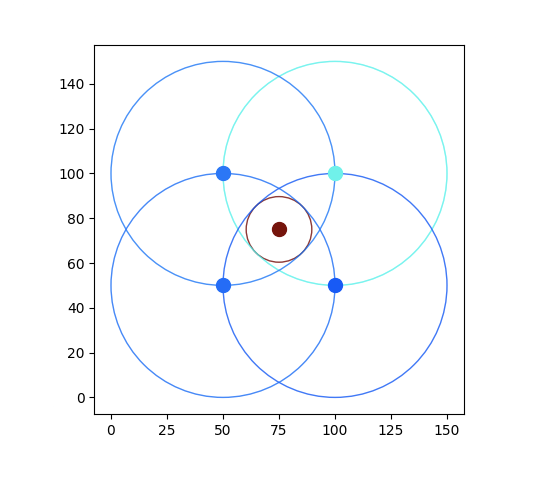
\includegraphics[width=0.8\textwidth]{Figuras/easy_trilateration.png}
        \captionsetup{margin=2cm}
        \caption[Herramienta gráfica de multilateración]{\href{https://github.com/agusalex/easy-trilateration}{\textbf{Herramienta gráfica de multilateración}}}
        \label{fig:libpython}
    \end{figure}

    \item \href{https://github.com/agusalex/rssi-filter-profiling}{\textbf{RSSI-Filter-Profiling}}: Herramienta que permite tomar múltiples capturas de perfilado, aplicar filtros como Kalman, mediana y promedio, realizar ajustes logarítmicos usando mínimos cuadrados y luego producir múltiples gráficas, incluyendo inversa y desviación estándar, comparando múltiples capturas de distintos dispositivos a la vez. También posee un combinador de gráficas, lo que permite tomar múltiples imágenes y convertirlas en una sola.

    \item \href{https://github.com/agusalex/ESP8266-sniffer-node}{\textbf{ESP8266-Sniffer-Node}}: Firmware para ESP8266 capaz de alternar entre el modo de captura de \textit{Probe Request} y el modo de subida de datos.

    \item \href{https://github.com/agusalex/ns3-rssi-trilateration}{\textbf{NS3-RSSI-Trilateration}}: Software que permite realizar perfilado y multilateración simulada usando NS3. Combina tanto \textbf{RSSI-Filter-Profiling} como \href{https://github.com/agusalex/easy-trilateration}{\textbf{Easy-Trilateration}} como submódulos de Git. Funciona aplicando un perfil de movilidad a un nodo, generando una captura simulada y luego graficando la reducción en la señal a medida que este se aleja, hallando los valores de \( A \) y \( N \). Posteriormente, permite simular un escenario de multilateración utilizando la herramienta mencionada. La idea de este software es ejecutar ambas simulaciones de manera sencilla.
\end{itemize}
\section{Hallazgos Principales}

Los experimentos realizados, tanto en entornos simulados como reales, han demostrado la capacidad de utilizar señales \acs{wifi} para localizar dispositivos móviles de manera efectiva. Este enfoque presenta una alternativa viable y de bajo costo a los sistemas basados en hardware especializado, ofreciendo una nueva herramienta para el análisis del comportamiento peatonal y vehicular en las ciudades.

A través de la investigación, se ha identificado la importancia de una disposición y configuración óptima de los nodos \textbf{Sniffer} para maximizar tanto la cobertura como la precisión de las estimaciones de ubicación. La interacción entre la disposición de los nodos y las características específicas del entorno urbano, como la cantidad de edificios, transeúntes y por sobre todo las interferencias electromagnéticas. Han demostrado ser un factores crítico en la eficacia de la localización.


\section{Limitaciones y Desafíos}

El proyecto enfrentó varias limitaciones técnicas y metodológicas. La precisión de las estimaciones de ubicación fue impactada por la interferencia inalámbrica y la variabilidad en la recepción de los dispositivos. Las limitaciones inherentes del hardware elegido y la infraestructura disponible para sostenerlo. Además, la práctica de la randomización de direcciones \acs{mac} en dispositivos modernos representa un desafío significativo para el seguimiento continuo de dispositivos a lo largo del tiempo.

\section{Recomendaciones para Futuras Investigaciones}
Para continuar avanzando en esta área, se considera importante:

\begin{itemize}
    \item Investigar en profundidad los efectos de la urbanización en la propagación de señales \acs{wifi} y desarrollar técnicas de corrección o compensación que mejoren la precisión en la estimación de la ubicación \cite{choi_2019_unsupervised}.
    \item Explorar utilizar \acs{gps}, para poder perfilar con precisión los nodos y así mejorar las estimaciones de ubicación obtenidas a través de \acs{wifi}.
    \item Desarrollar algoritmos de aprendizaje automático o alguna otra técnica para desenmascarar direcciones \acs{mac} que puedan identificar y seguir dispositivos a pesar de la randomización \acs{mac} \cite{baccichet2024mac}.
    \item Realizar experimentos adicionales en una variedad de entornos urbanos y con diferentes configuraciones de hardware para validar la robustez y adaptabilidad de las soluciones propuestas \cite{10.1007-978-3-030-11027}.
    \item Probar dichas técnicas con vehículos e instalaciones de \textit{Sniffers} sobre postes de luz para detectar vehículos estacionados\cite{yuansmartparking}.
    \item Explorar la posibilidad de detectar patrones de estacionamiento de automóviles, ciclistas que circulan por las calles y transeúntes en la vereda.
\end{itemize}

\section{Comentarios Finales}

La realización de esta tesis ha permitido explorar y expandir el conocimiento en el área de localización y seguimiento de dispositivos móviles en entornos urbanos, utilizando tecnología \acs{wifi} con micro-controladores de bajo costo. A pesar de enfrentar desafíos significativos, los resultados obtenidos proporcionan una base interesante para futuras investigaciones.

Mirando hacia adelante, es claro que la adopción de soluciones tecnológicas de tipo \textit{Smart Cities} jugará un papel fundamental en el diseño de las ciudades del futuro. Este trabajo contribuye a ese esfuerzo, sentando las bases para investigaciones futuras en el área de Smart Cities.
%\include{Capitulos/cap7}
%\chapter{Confección del documento de tesis}

\label{Capitulo_25}
%----------------------------------------------------------------------------------------
\section{Primeras consideraciones}

Llamamos \textbf{tesina} a una tesis de grado, realizada en un lapso breve, estimado en un año. Es de esperar que los resultados sean también acotados en relación, por ejemplo, a los de una tesis de maestría o doctorado, pero no por ello, tales resultados van a resultar menores o poco interesantes. En lo que resta del texto, tesina o tesis se consideran equivalentes, pero siempre referido a un trabajo monográfico de grado.

La tesis es el documento que resulta del trabajo de investigación y desarrollo del estudiante, y al igual que ese trabajo, las tesis son muy personales, en lo que respecta al contenido y su estructura. De todas maneras, y al igual que sucede en todos los escritos, se deben respetar ciertas pautas \cite{melendrez2006como}.

%----------------------------------------------------------------------------------------
%----------------------------------------------------------------------------------------

\section{Estructura de una tesis}
\label{Estructura}
%----------------------------------------------------------------------------------------
\subsection{Fase Inicial}

Una tesis es, en su forma general, un libro que versa acerca del conocimiento, o desarrollo, alcanzado a partir de cierto trabajo, es así que se pueden encontrar algunas características comunes a cualquier libro que se adquiera en un librería:

\begin{itemize}
	\item \textbf{Portada}: debe contener el título  y la información del autor, incluyendo el lugar donde se realizó, nombre del director o supervisor y el año de presentación.
	\item \textbf{Cita}: Opcional, cuando se quiere mostrar alguna fuente de inspiración o modelo de vida, tanto personal, cívico o profesional.
	\item \textbf{Resumen}: El Resumen es una síntesis del trabajo, y por lo tanto debe tener una estructura similar, debe ser breve, buscando no exceder la página. Se debe escribir en forma sintética, refiriéndose a  los objetivos, la  metodología,  resultados principales y las conclusiones.
	\item \textbf{Agradecimientos}: Esta página es opcional, los agradecimientos  y reconocimientos se escriben a continuación. No forma parte del proyecto.
	
	\item \textbf{Indice} se compone por las siguientes listas:
	\begin{itemize}
		\item {\textit{Lista de Abreviaciones}, empleadas en la tesina, es de gran ayuda al lector, que le evita perder el tiempo en la búsqueda, en el texto, de una abreviación que no recuerda.}
		\item \textit{Glosario.}
		\item \textit{Índice de figuras.}
		\item \textit{Índice de tablas.}
		\item \textit{Índice General.} Lista y localización de los títulos de todas las secciones y sub-secciones pertenecientes al cuerpo de la tesis.
	\end{itemize}
	\item \textbf{Dedicatoria}: Esta página es opcional, y en ella se dedica el trabajo a personas tanto físicas como jurídicas.
\end{itemize}
%----------------------------------------------------------------------------------------
\subsection{Cuerpo de la tesis}

A partir de aquí, empieza el desarrollo de la tesis. La estructura difiere de tesis en tesis, pero una tesis bien escrita debe tener un hilo conductor, empezando por el problema y finalizando con las conclusiones y recomendaciones. En el medio, se leen el \textit{Objeto de Estudio}, los \textit{Objetivos} del trabajo de \ac{id}, las \textit{Tareas}, \textit{Metodología}, \textit{Resultados} y \textit{Discusión}.

Para profundizar sobre las relaciones existentes entre estas etapas, se puede consultar \cite{melendrez2006como}. Es importante notar que, de estas relaciones surge naturalmente la estructura de la tesis y esa estructura se vé en el Índice General. En lugar de dar inicio a la escritura en la introducción, Umberto Eco propone empezar por el índice, de manera tal que se pueda definir rápidamente el marco de trabajo \cite{eco2015write}.

\paragraph{La Discusión}
Este apartado merece una reflexión aparte. Puede  confundirse la \textit{Discusión} de un trabajo, con las \textit{Conclusiones} de mismo, o considerarlos equivalentes. No es así, son cuestiones diferentes, y  ambas son los apartados más importantes de la tesis. Por una parte la \textbf{Discusión} analiza los resultados obtenidos, busca la utilidad de ellos y los pone en contraposición con la literatura. Es el apartado donde se expone el  conocimiento generado, o el nuevo desarrollo tecnológico, y para ello, se contrasta con trabajos realizados por otros grupos del ámbito científico-tecnológico. Es posible encontrar los \textbf{Resultados} y la \textbf{Discusión} en un mismo capítulo.
Por otra parte, mediante las \textbf{Conclusiones}, que corresponden a la fase final de la tesis, se indican los logros en relación con los objetivos, problemas o preguntas planteadas, que se derivan de los resultados obtenidos.
%----------------------------------------------------------------------------------------

\subsection{Fase Final}

En la Fase Final de la tesis se encuentran las \textit{Conclusiones} y \textit{Recomendaciones}. En algunos casos, se las incluye en un único capítulo, pero conceptualmente deben abordarse en forma separada. Ibañez Brambila \cite{brambila2000manual} plantea sobre estos apartados que deben 
\begin{itemize}
	\item \textbf{Conclusión}: Representan un elemento esencial de la tesis puesto que es ahí donde se hacen constar los resultados obtenidos y la aportación de éstos en el ámbito estudiado. Aquí se da respuesta a los objetivos e hipótesis planteadas. La conclusión debe ser breve, respecto de la extensión del contenido, pero muy explícita, y donde “se manifiestan el valor del estudio, así como el dominio que se tiene del tema”
	\item \textbf{Recomendaciones}: Éstas se redactan después de las conclusiones. Se definen como sugerencias que se formulan con el propósito de indagar en el tema de investigación. Se puede recomendar otra dimensión del problema, o incluso otra forma  de  abordarlo.  Básicamente  se  trata  de  aportar  recomendaciones  para investigaciones futuras.
\end{itemize}

%----------------------------------------------------------------------------------------

\subsection{Referencias y Anexos.}

Terminando la tesis, se encuentran  los \textbf{Anexos}, con información que aporta y complementa a la tesis, pero que no tiene la relevancia para estar en el cuerpo principal, por algún motivo. Dentro de los anexos pueden encontrarse ejemplos de resultados, desarrollos teóricos extendidos, los cuales aparecen en el cuerpo de manera reducida, entre otras opciones. Por último se encuentra la lista de \textbf{Referencias}, es decir, la bibliografía sobre la cuál se basa y discute la tesis.

%----------------------------------------------------------------------------------------
%----------------------------------------------------------------------------------------

\section{Ejemplos de estructura}

En \ref{Estructura} se hizo un recorrido por las partes y apartados constitutivos de una tesis. A continuación se darán algunos ejemplos de estructuras, limitados al cuerpo de la tesina.
%----------------------------------------------------------------------------------------
\subsection{Ejemplo 1}
El ejemplo 1 es sumamente genérico, con una estructura que se puede encontrar en una tesis, pero también en los artículos científicos.

\begin{itemize}
	\item \textit{Capítulo 1: Introducción}
	\item \textit{Capítulo 2: Marco teórico y Estado del Arte}
	\item \textit{Capítulo 3: Objetivos}
	\item \textit{Capítulo 4: Metodología}
	\item \textit{Capitulo 5: Resultados}
	\item \textit{Capítulo 6: Discusión}
	\item \textit{Capítulo 7: Conclusiones}
	\item \textit{Capítulo 8: Recomendaciones}	

\end{itemize}
%----------------------------------------------------------------------------------------	
\subsection{Ejemplo 2}
El ejemplo 2 se extrajo de una tesis que fuera presentada para cumplir los requerimientos de la carrera de grado en Ciencias Biológicas, School of Science, Kathmandu University.

\begin{itemize}
	\item \textit{Capítulo 1: Introducción}
	\item \textit{Capítulo 2: Revisión Bibliográfica}
	\item \textit{Capítulo 3: Materiales y Métodos}
	\item \textit{Capítulo 4: Resultados y Discusión}
	\item \textit{Capítulo 5: Conclusión}
	\item \textit{Capítulo 6: Recomendaciones}
\end{itemize}
%----------------------------------------------------------------------------------------
\subsection{Ejemplo 3}
También se puede pensar en una estructura más adecuada al lugar y trabajo particular desarrollado

\begin{itemize}
	\item \textit{Capítulo 1: Introducción a los tópicos de la tesis}
	\item \textit{Capítulo 2: Teoría y estado de arte}
	\item \textit{Capítulo 3: Dispositivo experimental de Laboratorio}
	\item \textit{Capítulo 4: Detalles del experimento 1}
	\item \textit{Capítulo 5: Detalles del experimento 2}
	\item \textit{Capítulo 6: Discusión de los resultados experimentales}
	\item \textit{Capítulo 7: Conclusión y futuras direcciones de estudio}
	
\end{itemize}	

%----------------------------------------------------------------------------------------
%----------------------------------------------------------------------------------------

\subsection{Algunas reflexiones. }

(En construcción)
La tesis posee una estructura lineal, que está dada, según se comentó previamente,  por  su estructura, (capítulos, secciones, subsecciones). No obstante la información que esta contiene fluye entre sus partes. Cada capítulo requiere de los anteriores, y todos ellos vuelven, necesariamente, al primero, \emph{Estado del Conocimiento}. Ver figuta \ref{fig:flujo}.

\begin{figure}[th]
	\centering
	\includegraphics[width=0.6\textwidth]{Figuras/flujo}
	\captionsetup{margin=2cm}
	\caption[Flujo de lectura de la tesis]{La tesis, por  sobre su estructura lineal, necesita un flujo de información más complejo.  }
	\label{fig:flujo}
\end{figure}

Tenga en consideración, entonces,  que el desarrollo de la tesis, al igual que los trabajos realizados necesitan de todo el contenido. Por ejemplo, el Estado de Conocimiento es el paraguas sobre el que se realiza todo el trabajo, los resultados son consecuencia de la metodología, que a su vez tienen que ver con los Objetivos que se persiguen y debe poder relacionarse con el conocimiento existente. La Discusión existe gracias a los resultados, y en ella se estudian los nuevos descubrimientos en relación a lo que se sabe, considerando las condiciones que impone la metodología. Todo lleva a las conclusiones del estudio, y a el camino a seguir que se recomienda. 
%----------------------------------------------------------------------------------------
%----------------------------------------------------------------------------------------

\section{Características y convenciones de la tesis}\label{Convenciones}

Para aprovechar al máximo esta plantilla, existen algunas convenciones que tal vez desee seguir.

Una de las cuestiones más importantes, y más difíciles de controlar en un documento tan largo, como una tesis, es la coherencia. Usar ciertas convenciones y formas de hacer las cosas, como usar una lista de tareas, facilita el trabajo. Por supuesto, esto es opcional y puede adoptar su propio método.

%----------------------------------------------------------------------------------------

\subsection{Formato de Impresión}

Esta plantilla se configura para un papel A4, que es el tamaño estándar en Argentina y es el requerido en la presentación de la tesis. 
 
La plantilla está diseñada para impresión simple,  en una cara de la hoja. Se declara al principio del archivo \file{tesina.tex} el formato de la tesina \emph{report}:
\begin{verbatim}
	\documentclass{report}
\end{verbatim}

y el ajuste de página y  márgenes, 
\begin{verbatim}
	\usepackage[paper=a4paper,top=2in, bottom=1.5in, left=1in, right=1in]{geometry}
\end{verbatim}

 Para las tesis que se impriman, es preferible un formato de impresión doble faz, imprimiendo en el anverso y el reverso de las hojas, para ello comente las dos primeras líneas de código y des-comente la línea 
\begin{verbatim}
	\documentclass[twoside]{report}.
\end{verbatim}


Los encabezados de las páginas contienen el nombre del capítulo en el lado interior. y el número de página en el lado exterior (por lo que es fácil desplazarse hasta la página que desea).

El texto está configurado en 11 puntos por defecto con un espacio de una sola línea, nuevamente, puede ajustar el tamaño y espaciado del texto si lo desea, o necesita, usando las opciones. Para ello al comienzo de \file {main.tex}, se encuentra el bloque \emph{CONFIGURACIÓN INTERLINEA}.


%----------------------------------------------------------------------------------------
\subsection{Seccionado y Subseccionado}


Debes dividir su tesis en secciones y subsecciones de un tamaño adecuado para una correcta comprensión del texto. En la compilación, \LaTeX{} genera automáticamente una tabla de contenidos al compilar  todos los comandos \verb|\chapter{}|, \verb|\section{}| y \verb|\subsection{}| que escribe en el código fuente de su tesis.

La tabla de contenido solo debe enumerar las secciones en tres (3) niveles. Un \verb|\chapter{}| es el nivel cero (0). Una \verb|\section{}| es el nivel uno (1) y por lo tanto una \verb|\subsection{}| es el nivel dos (2). En su tesis es probable que incluso emplee \verb|\subsubsection{}|, que es el nivel tres (3).

%----------------------------------------------------------------------------------------
\subsection{Referencias}


El paquete \code{bibtex} se usa para formatear la bibliografía e insertar referencias como la siguiente \verb*|\cite{Referencia1}|: \cite{Referencia1}. Para simplificar se emplean las opciones por defecto de \code{bibtex}, las citas se organizan de acuerdo al orden de aparición en el cuerpo de la tesis. Las referencias múltiples están separadas por comas (por ejemplo, \cite{Referencia2, Referencia1}).

Las referencias científicas deben ir \emph{antes} del signo de puntuación si lo hay. Lo mismo ocurre con las notas al pie \footnote{Como esta nota al pie, aquí abajo en la parte inferior de la página.}. Puede modificar esto, pero lo más importante es mantener la convención consistente a lo largo de la tesis. Las notas al pie de página deben ser oraciones completas y descriptivas (comenzando con una letra mayúscula y terminando con un punto).

Existen otros paquetes que complementan a \code{bibtex} o \code{biblatex}, como por ejemplo \emph{natbib}, o que los reemplazan como \emph{biber}, ofreciendo mayores funcionalidades. Puede emplear el paquete de su preferencia.


%----------------------------------------------------------------------------------------









\section{Bienvenid@ y Gracias}
Bienvenida/o a esta plantilla de tesis en \LaTeX{}. Una plantilla simple de usar, para escribir su tesis usando el sistema de tipografía \LaTeX. 

Si va a escribir una tesis técnica o matemática, es recomendado realizarla en \LaTeX{}, de manera tal de concentrar los esfuerzos en lo esencial, sin preocuparse por cuestiones de formato, ni acceso a determinado procesador de textos.

\LaTeX{} puede componer fácilmente documentos de forma profesional que se ejecutan en cientos o miles de páginas. Con comandos de marcado simples, establece automáticamente en tabla de contenido,  márgenes, encabezados y pies de página, mantiene el formato consistente y atractivo. Una de sus principales fortalezas es la forma en que pueden componer fácilmente  fórmulas  matemáticas, incluso las expresiones más \emph{complejas}. Si esas ecuaciones son  problemas matemáticos  horriblemente retorcidos y difíciles, que solo pueden resolverse en una supercomputadora, al menos puede contar con \LaTeX{} para que se vean lindos.


%----------------------------------------------------------------------------------------
\section{Aprendiendo \LaTeX{}}

\ LaTeX {} no es un programa \textsc{wysiwyg} (What You See is What You Get - Lo que ve es lo que obtiene), a diferencia de los procesadores de texto como Microsoft Word o Pages de Apple. En cambio, un documento escrito para \LaTeX{} es en realidad un archivo de texto plano, simple, \emph {sin formato}. Para asignar formatos a lo escrito, se le dice a \LaTeX{}, cómo se quiere el formato en el documento terminado, escribiendo comandos simples entre el texto, por ejemplo, si quiere usar \emph{texto en cursiva para enfatizar}, se escribe el comando \verb | \emph{texto} |  con el texto que se quiere enfatizar  entre las llaves. Esto significa que \LaTeX{} es un lenguaje de \textit{marcado}, con cierto parecido  al HTML.



\subsection{Una (no tan corta) Introducción a \LaTeX{}}

Si es nuevo en \LaTeX{}, hay un libro electrónico muy bueno, disponible gratuitamente en línea como un archivo PDF, llamado \textit {The Not So Short Introduction to \LaTeX{}}. El título del libro suele acortarse a  \emph{lshort}. Puede descargar la última versión (ya que se actualiza ocasionalmente) desde aquí:

\url{http://mirrors.ctan.org/info/lshort/spanish/lshort-a4.pdf}

Se recomienda tomar un poco de su tiempo para aprender a usar  \LaTeX{} creando varios documentos pequeños de "prueba" u observando de cerca algunos ejemplos. Hacer el esfuerzo ahora significa que no estará atrapado aprendiendo el sistema cuando lo que \emph{realmente} necesita hacer es escribir su tesis.


\subsection{Una Guía Corta de Matemáticas para \LaTeX{}}

Si está escribiendo una tesis técnica o matemática, es posible que desee leer el documento de la AMS (American Mathematical Society) llamado \textit{A Short Math Guide for \ LaTeX {}}. Se puede encontrar en la dirección:
\url {https://ctan.dcc.uchile.cl/info/short-math-guide/}

Algunos ejemplos de ecuaciones, pueden ser \emph{en la línea}, escribiendo \verb*|$\int f(\alpha)~d\alpha$| obtendrá la ecuación en línea  $\int f(\alpha)~d\alpha$. Note que la ecuación se escribe entre \verb|$| y \verb|$|. La misma ecuación puede centrarse en la página escribiéndola entre \verb|$$| y \verb|$$|. $$\int f(\alpha)~d\alpha$$. No es la única forma de ingresar ecuaciones,  por ejemplo,

\begin{lstlisting}[basicstyle=\small,tabsize=4]
	\begin{gather}
		si ~ \not ~  C(s,a,a') < \bar{R} \tau  \Rightarrow ~  \Bigg \{ 
			{\begin{matrix}
				a \rightarrow  \{a,a'\} ~ en ~ s  \\
				sino \\
				\{a,a'\} \rightarrow a ~en~ s
			\end{matrix}}
	\end{gather}
\end{lstlisting}
 
 devuelve como resultante:
 
 \begin{gather}
 	si ~ \not ~  C(s,a,a') < \bar{R} \tau  \Rightarrow ~  \Bigg \{ 
 		{\begin{matrix}
 			a \rightarrow  \{a,a'\} ~ en ~ s  \\
 			sino \\
 			\{a,a'\} \rightarrow a ~en~ s
 		\end{matrix}}
 \end{gather}

Otro ejemplo, 

\begin{equation}
	\label{eq: gate}
	G(t) = \frac{t}{\tau_{ampa}} e^{-\frac{t}{\tau_{ampa}} } ~H(t)
\end{equation}

en este último ejemplo \ref{eq: gate}, se agregó un \emph{label}  para hacer referencia a la ecuación en el texto. El código para declarar la ecuación \ref{eq: gate} es: 

\begin{lstlisting}[basicstyle=\small,tabsize=4]
	\begin{equation}
		\label{eq: gate}
		G(t) = \frac{t}{\tau_{ampa}} e^{-\frac{t}{\tau_{ampa}} } ~H(t)
	\end{equation}
\end{lstlisting}
 

Es muy grande la diversidad de símbolos matemáticos, los cuales se pueden encontrar fácilmente buscando en la web, por ejemplo \url{http://math.mit.edu/~dspivak/files/symbols-all.pdf} ó también \url{http://www.sunilpatel.co.uk/latex-type/latex-math-symbols/}

%----------------------------------------------------------------------------------------
\subsection{Una guía corta sobre Tablas}

Las tablas son una forma importante de mostrar sus resultados, a continuación se muestra una tabla de ejemplo que se generó con este código:

{\small
	\begin{lstlisting}[basicstyle=\small,tabsize=4]
		\begin{table}
			\caption{Los efectos de los tratamientos X e Y en los cuatro grupos estudiados.}
			\label{tab:tratamientos}
			\centering
			\begin{tabular}{l l l}
				\toprule
				\tabhead{Grupos} & \tabhead{Tratamiento X} & \tabhead{Tratamiento Y} \\
				\midrule
				1 & 0.2 & 0.8\\
				2 & 0.17 & 0.7\\
				3 & 0.24 & 0.75\\
				4 & 0.68 & 0.3\\
				\bottomrule\\
			\end{tabular}
		\end{table}
	\end{lstlisting}
}

\begin{table}
	\caption{Los efectos de los tratamientos X e Y en los cuatro grupos estudiados.}
	\label{tab:tratamientos}
	\centering
	\begin{tabular}{l l l}
		
		\tabhead{Grupos} & \tabhead{Tratamiento X} & \tabhead{Tratamiento Y} \\
		
		1 & 0.2 & 0.8\\
		2 & 0.17 & 0.7\\
		3 & 0.24 & 0.75\\
		4 & 0.68 & 0.3\\
		
	\end{tabular}
\end{table}

Puede hacer referencia a tablas con \verb|\ref{<etiqueta>}| donde la etiqueta se define dentro del entorno de la tabla. Consulte \file{cap2.tex} para ver  ejemplos de etiquetado y citas (por ejemplo, el correspondiente a esta Tabla ~ \ref{tab:tratamientos}).

%----------------------------------------------------------------------------------------

\subsection{Una guía corta sobre Figuras}

Es de esperar que haya figuras en su tesis , y que deben localizarse en la carpeta \emph{Figuras}. Se pueden emplear formatos pdf, jpg and png. Una forma de insertar figuras en su tesis es usar una plantilla de código como la siguiente:

\begin{lstlisting}[basicstyle=\small,tabsize=4]
	\begin{figure}
		\centering
		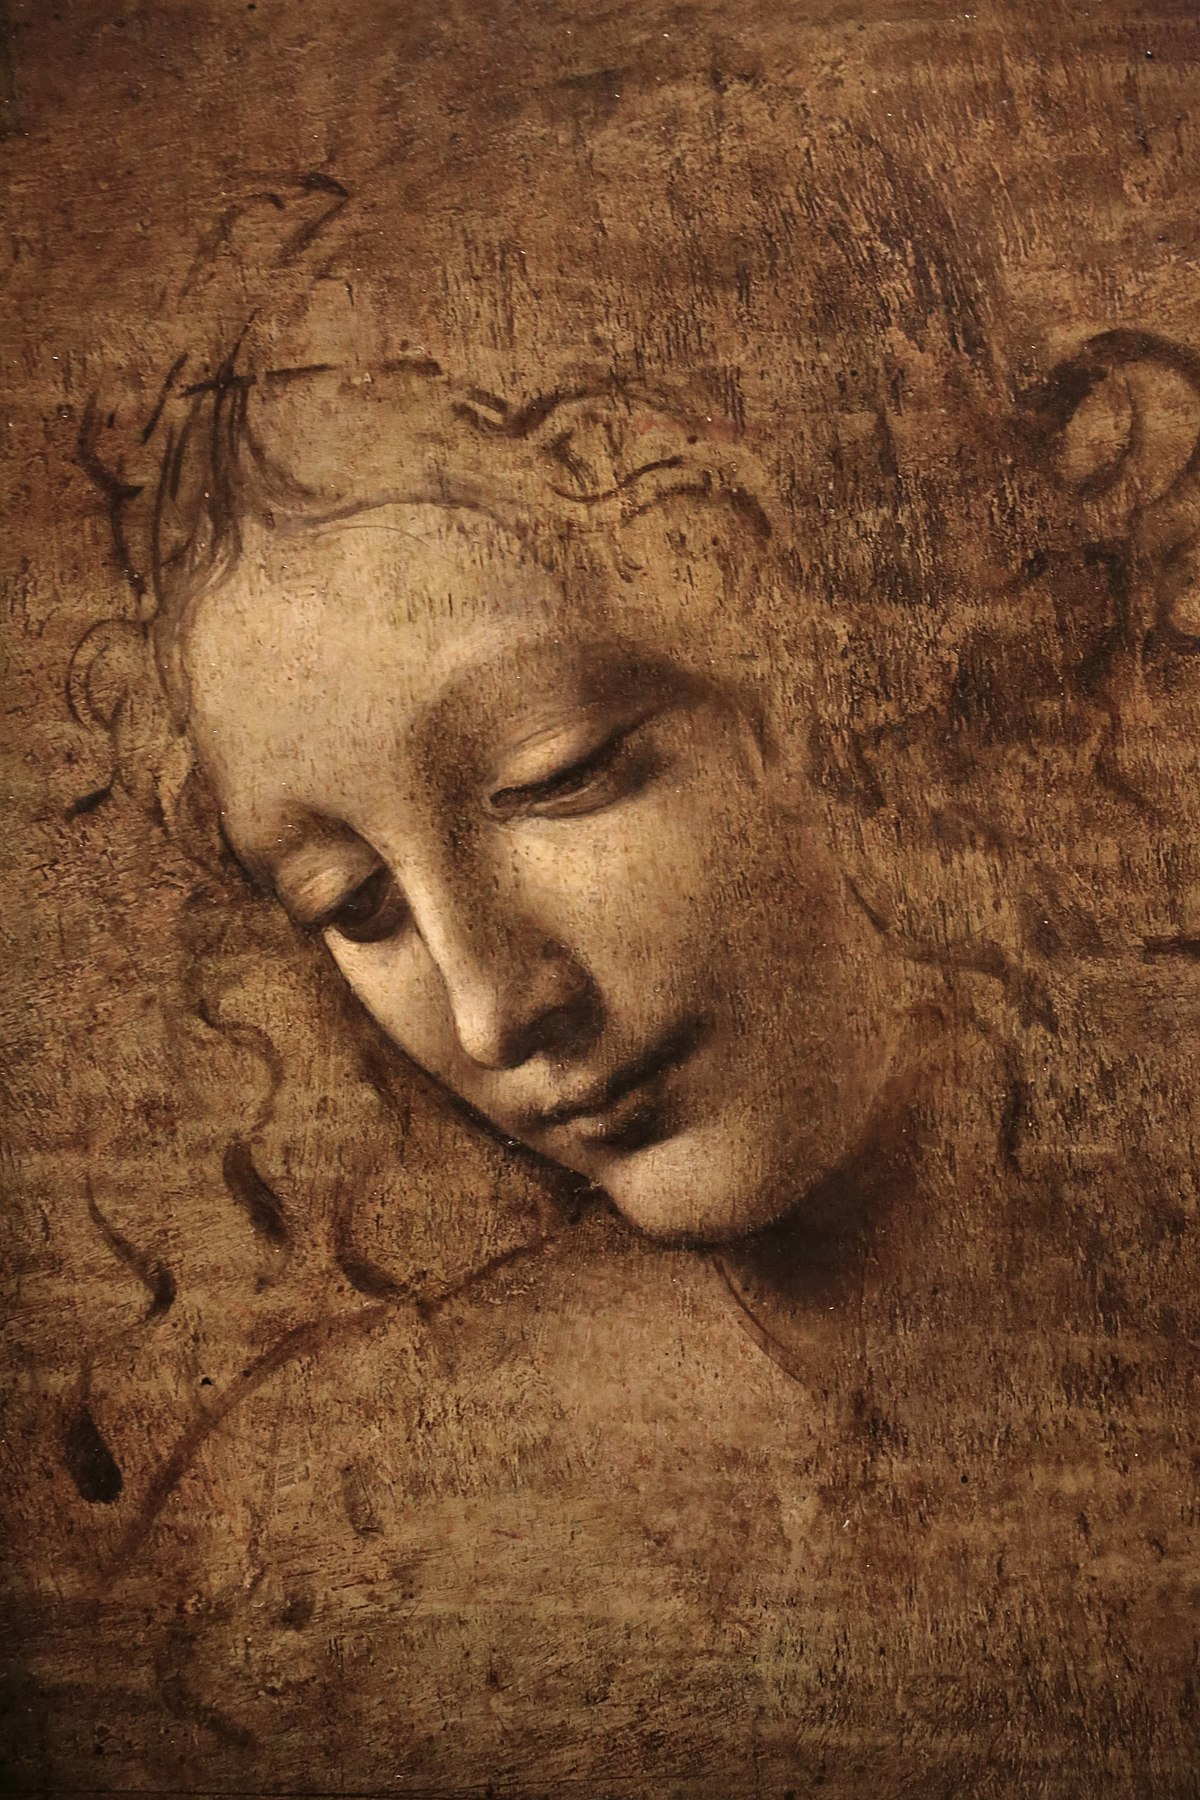
\includegraphics[width=0.6\textwidth]{Figuras/scapigliata}
		\captionsetup{margin=4cm}
		\caption[La Scapigliata]{La Scapiliata, una pintura al oleo sin ....}
		\label{fig:Scapigliata}
	\end{figure}
\end{lstlisting}


\begin{figure}[th]
	\centering
	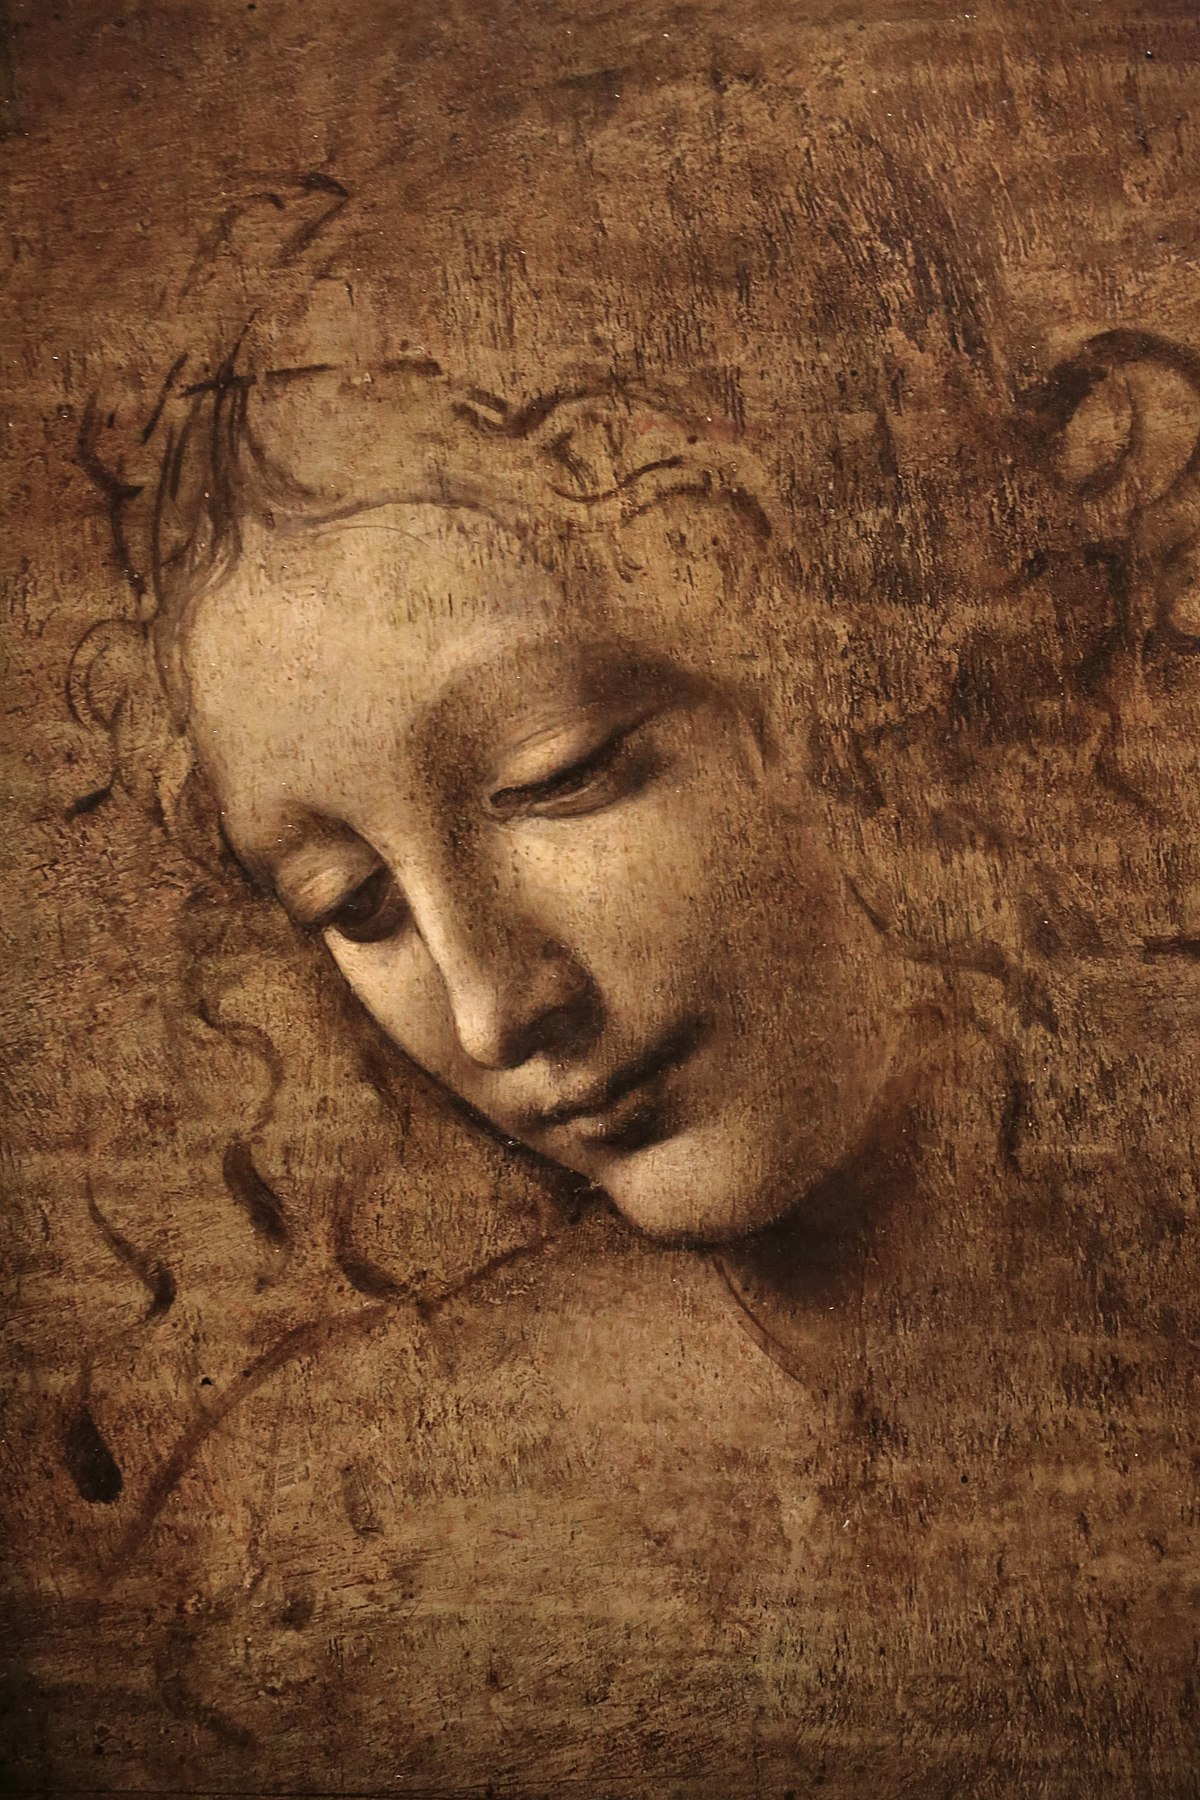
\includegraphics[width=0.4\textwidth]{Figuras/scapigliata}
	\captionsetup{margin=4cm}
	\caption[La Scapigliata]{La Scapiliata, una pintura al oleo sin terminar de fines del Renacimiento. No se conoce el autor, algunos historiadores atribuyen la autoría a Leonardo da Vinci.}
	\label{fig:Scapigliata}
\end{figure}

\LaTeX{} ubica las imágenes dependiendo del espacio que exista en la página. Algunas veces no hay lugar  suficiente para colocar una imagen en donde se declara \verb*|\begin{figure}|, en consecuencia \LaTeX{} la ubica en la parte superior de la siguiente página.
	
	Las figuras deben tener subtítulos los cuales deben ser explicativos y sintéticos.  También se pueden referenciar en el texto (como con la Figura ~ \ref{fig:Scapigliata}). La declaración \verb|\caption| posee dos partes, la primera parte, dentro de los corchetes es el título que aparecerá en el \emph{Índice de figuras}, por lo que debe ser breve. La segunda parte entre llaves debe contener el título más largo y la descripción de la figura. También se puede encuadrar el título de la figura referido al margen de la hoja, para ello debe emplear  \verb*|\captionsetup{margin=4cm}|. 
	
	
	
	También es posible cambiar la posición del comentario, por ejemplo, con la siguiente plantilla de código 
	
	\begin{lstlisting}[basicstyle=\small,tabsize=4]
		\begin{SCfigure}[0.5][h]
			\centering
			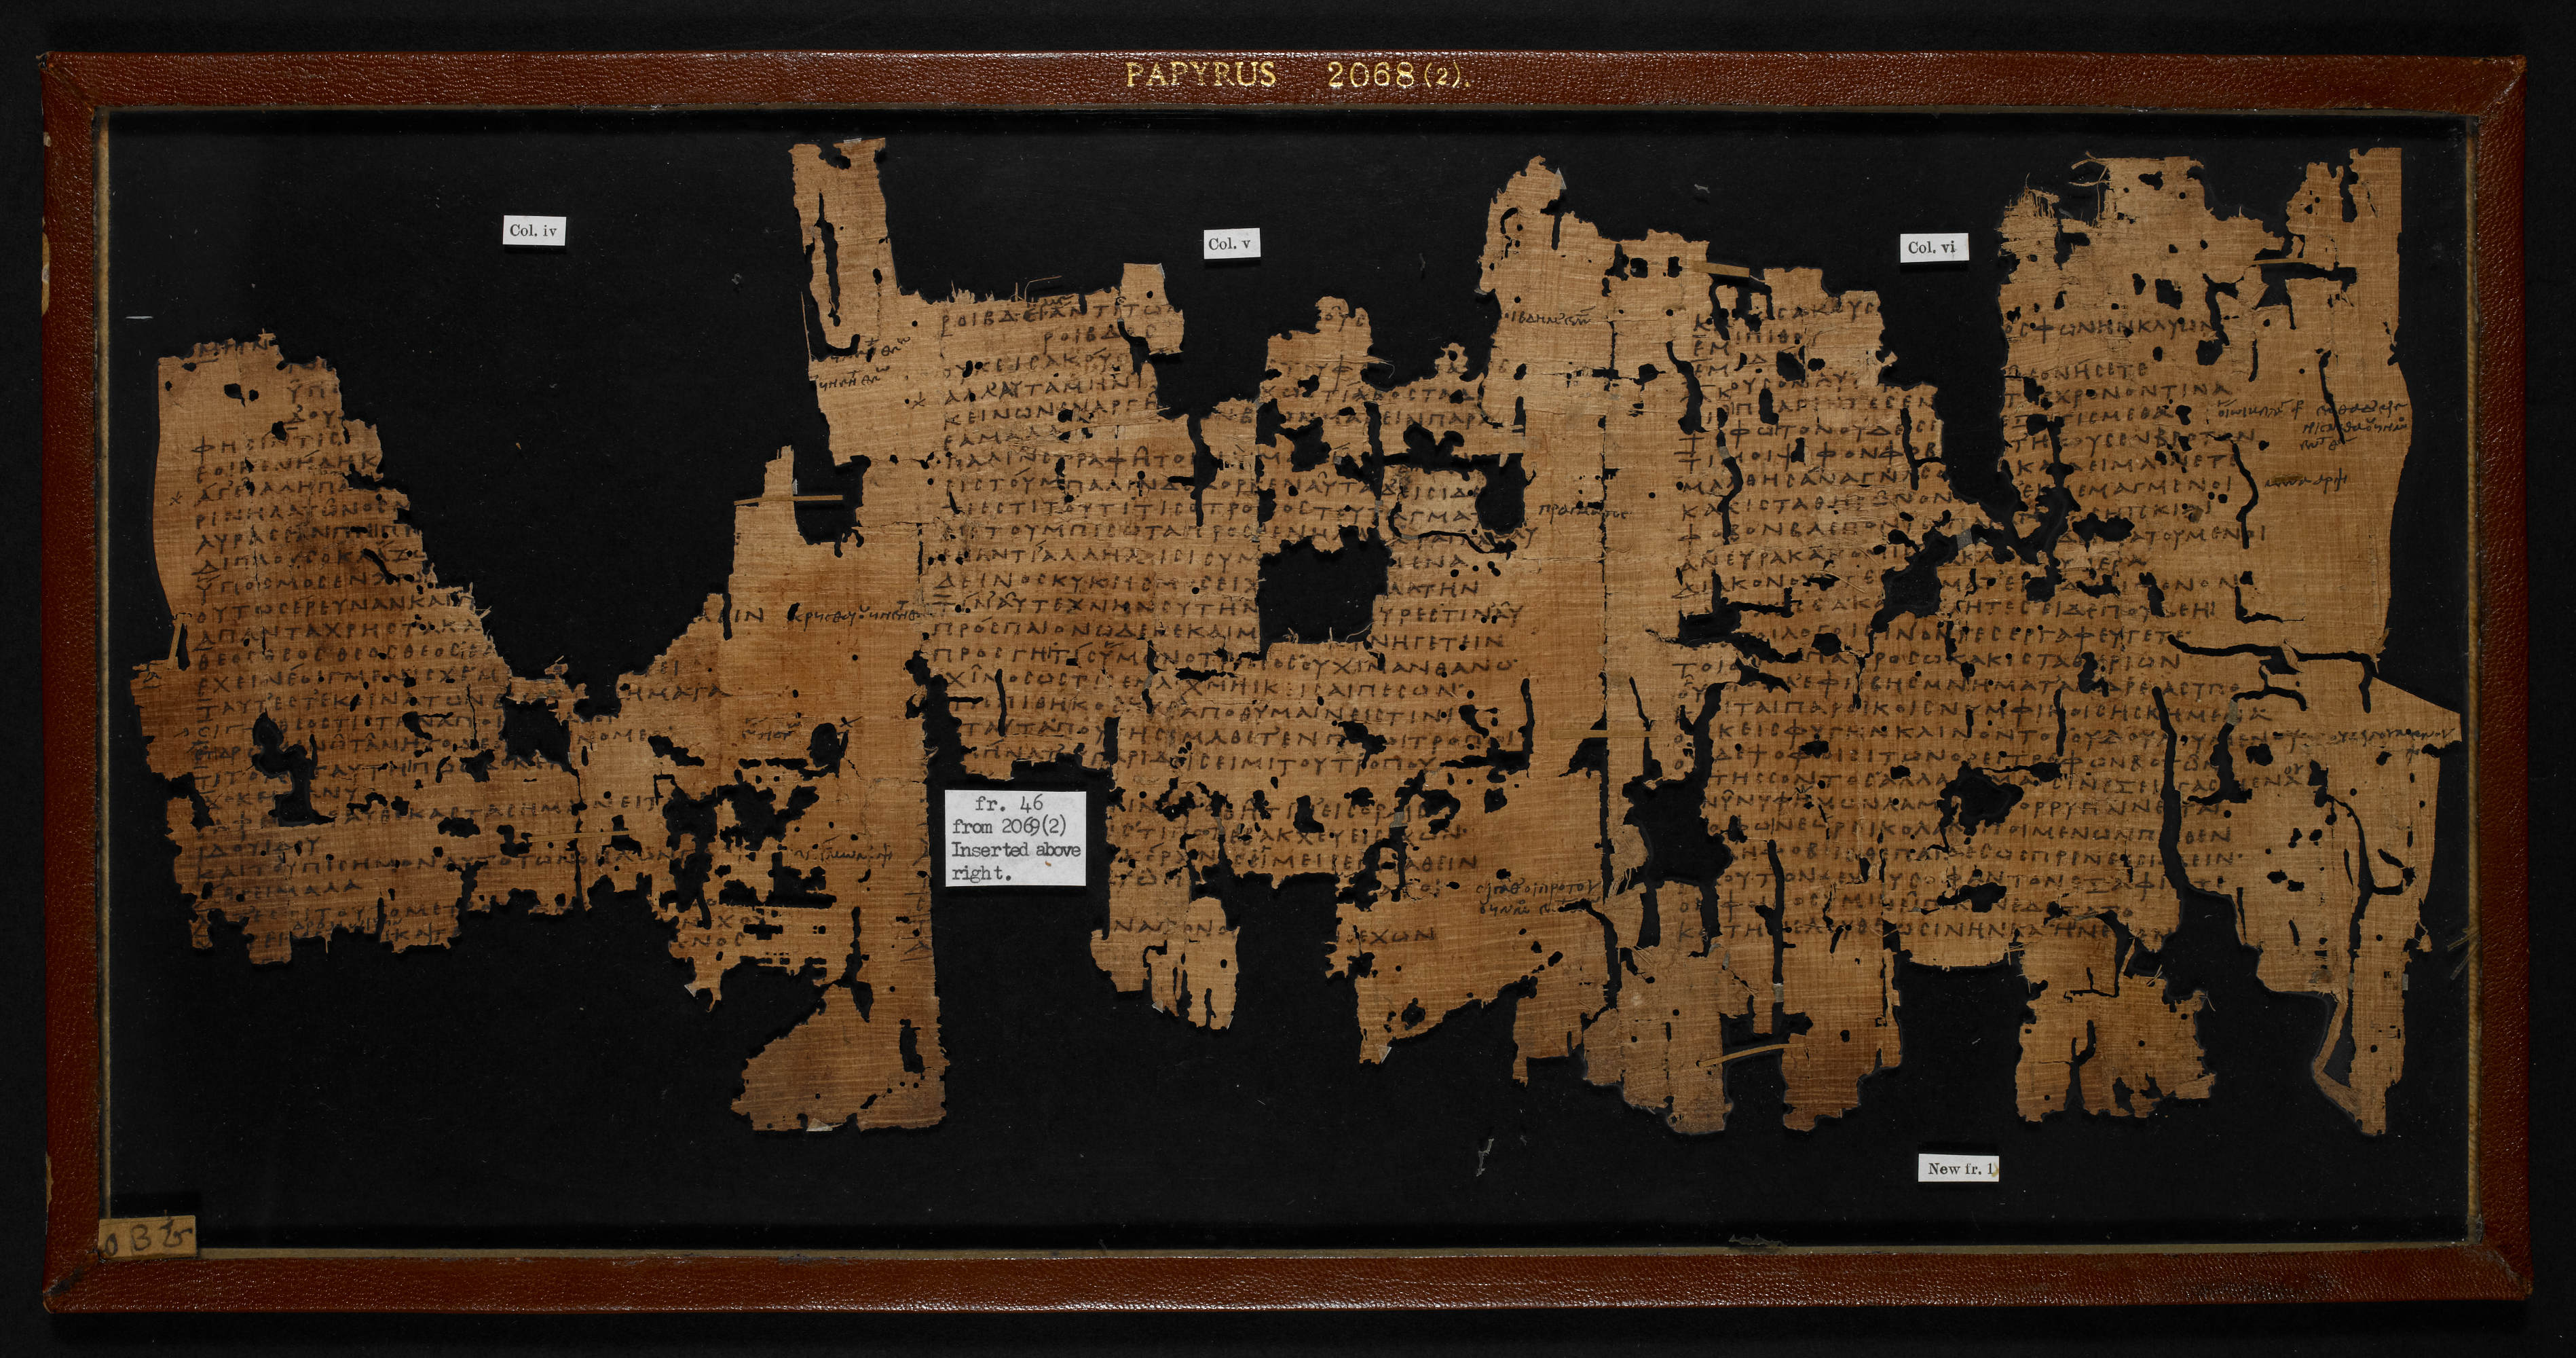
\includegraphics[width=0.6\textwidth]{Figuras/papyrus_sofocles}
			\caption[Ichneutae ....
			\label{fig:diag}
		\end{SCfigure}
	\end{lstlisting}
	
	se obtiene el resultado en la Figura \ref{fig:diag}, donde los comentarios de aparecen a la derecha.
	
	
	\begin{SCfigure}[0.5][h]
		\centering
		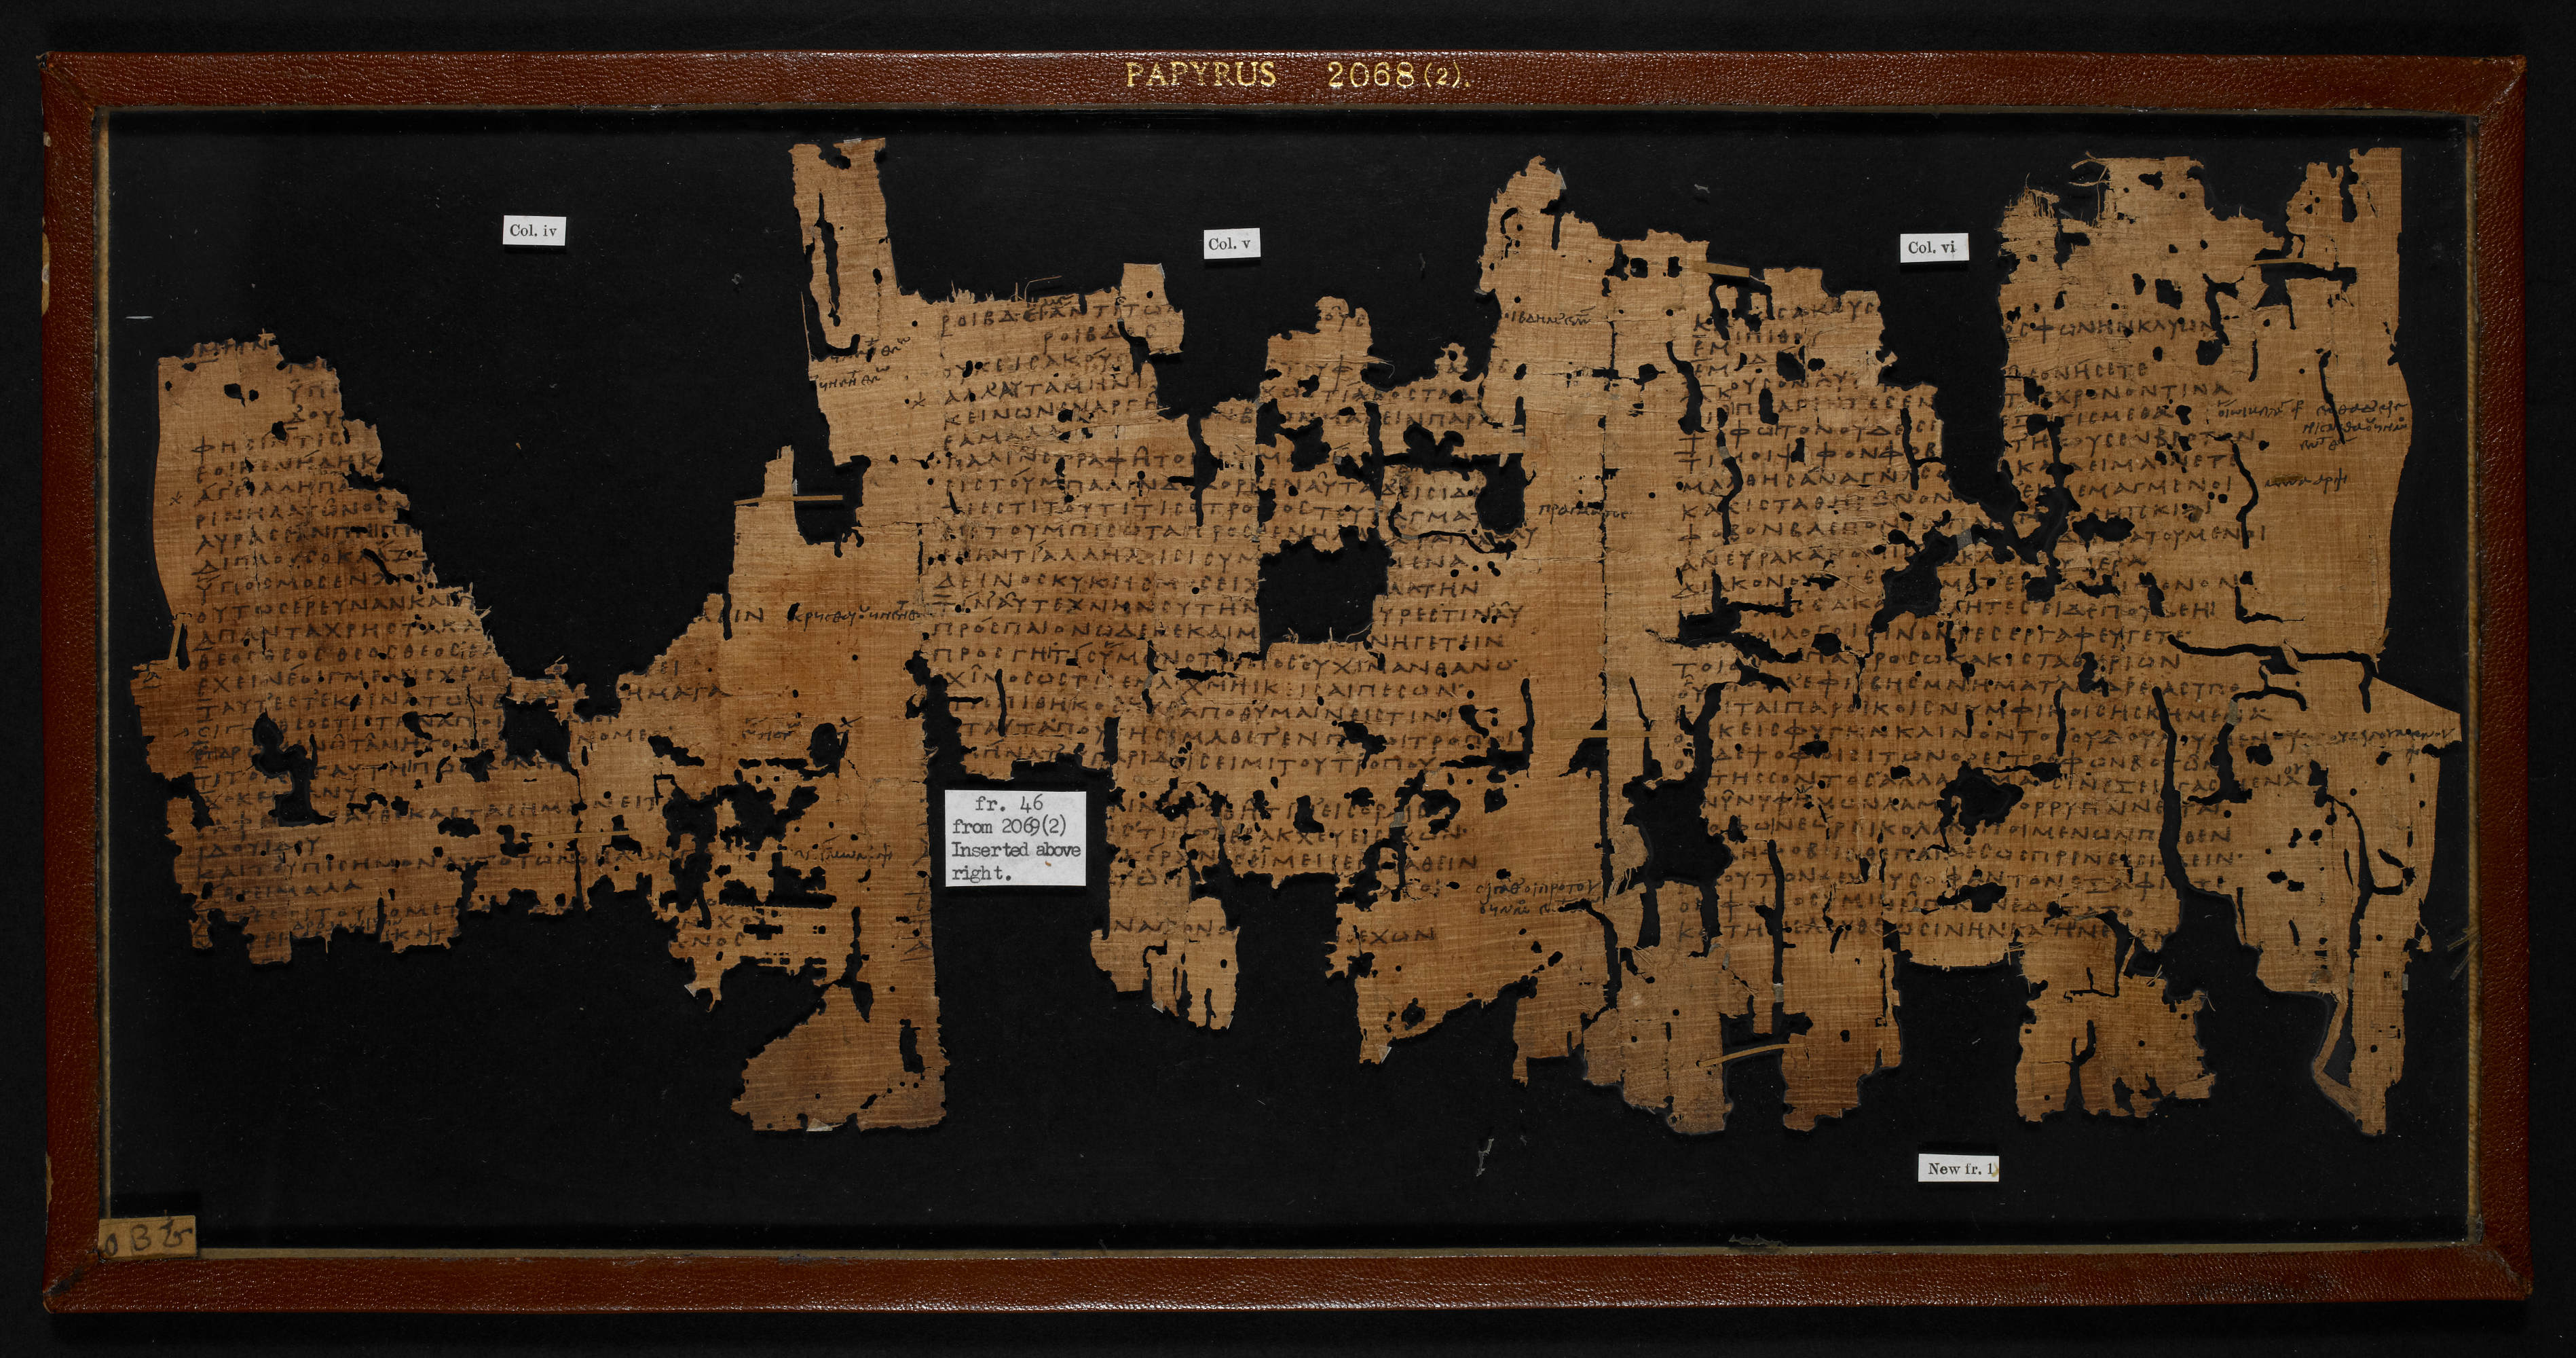
\includegraphics[width=0.6\textwidth]{Figuras/papyrus_sofocles}
		\caption[Ichneutae, o Perseguidores sátiros.]{Ichneutae, o Perseguidores sátiros. Fragmento del manuscrito del dramaturgo ateniense Sófocles. (Museo Británico)}
		\label{fig:diag}
	\end{SCfigure}
	
	%----------------------------------------------------------------------------------------
	\subsection{Una guía corta sobre Algoritmos}
	
	
	\begin{algorithm}[H]
		\label{alg:ejemplo1}
		\SetAlgoLined
		\KwData{$G=(X,U)$ de forma tal que $G^{tc}$ es un orden.}
		\KwResult{Escriba aquí el resultado }
		inicialización\;
		\While{condición}{
			instrucciones\;
			\eIf{condición}{
				instrucción1\;
				instrucción2\;
			}{
				instrucción3\;
			}
		}
		\caption{Cómo escribir una algoritmo}
	\end{algorithm}
	\
	
	Para la escritura de algoritmos existen diferentes posibilidades. En esta plantilla se empleó \verb*|\usepackage{listings}| para mostrar código desde un archivo. \emph{listings} permite listar código en diferentes lenguajes, por ejemplo, en el directorio \file{Codigo} se encuentra el archivo \file{c.c}.
	
	Mediante \verb*|\lstinputlisting[numbers=left, language=c]{Codigo/c.c}| se obtiene
	
	\lstinputlisting[numbers=left, language=c]{Codigo/c.c}
	
	\textbf{Un inconveniente con \emph{listings} es no tener una buena compatibilidad con UNICODE.}
	\\
	
	En muchos casos es preferible presentar un pseudocódigo que muestre en forma genérica la implementación de determinada deducción. Para ello el paquete \emph{algorithm2e} ofrece una alternativa muy conveniente. Se invita a mirar el archivo \file{Capitulos/cap3.tex} para observar el código que permite el resultado del Algoritmo \ref{alg:ejemplo1}
	
	
	
	%----------------------------------------------------------------------------------------

\section{Empiece a trabajar con esta Plantilla}

Si está familiarizado con \LaTeX{}, entonces debería explorar la estructura de directorios de la plantilla y luego proceder a cargar  su propia información en el archivo \file{tesina.tex}.  La sección \ref{CargaArchivo} en la página \pageref{CargaArchivo} le ayudará a hacer esto. Asegúrese de leer también la sección \ref{Convenciones} sobre las convenciones de tesis para aprovechar al máximo esta plantilla.

\subsection{Sobre esta Plantilla.}

Esta plantilla de tesis en \LaTeX{} tiene sus orígenes alrededor de un archivo de estilo \LaTeX{} creado por Steve R.  Gunn de la Universidad de Southampton (Reino Unido), Departamento de Electrónica y Ciencias de la Computación. Puede encontrar el archivo de estilo original en el sitio:
\url{http://www.ecs.soton.ac.uk/~srg/softwaretools/document/templates/}

A su vez, Sunil Patel tomó el archivo de clase \file{ecsthesis.cls} de Steve y lo modificó creando un marco esqueleto y una estructura de carpetas para colocar los archivos de tesis. La plantilla resultante se puede encontrar en el sitio de Sunil aquí: \url{http://www.sunilpatel.co.uk/thesis-template}

Se tomó la plantilla de Sunil, se la simplificó, y se adaptó a la presente plantilla, que conforma el modelo para la Tesina de Licenciatura de Sistemas de la Universidad Nacional de General Sarmiento. 
%----------------------------------------------------------------------------------------

\section{¿Qué incluye esta Plantilla?}

\subsection{Carpetas}
Esta plantilla viene como un único archivo zip que se expande a varios archivos y carpetas. Los nombres de las carpetas son en su mayoría autoexplicativos:

\keyword{Apendices}: esta es la carpeta donde coloca los apéndices. Cada apéndice debe ir en su propio archivo \file{.tex} separado. En el directorio se incluyen un ejemplo y una plantilla.

\keyword{Capítulos}: esta es la carpeta donde se encuentran el resumen y los capítulos de tesis. Una tesis suele tener unos seis capítulos, aunque no existe una regla estricta al respecto. Cada capítulo debe ir en su propio archivo \file{.tex} separado y se pueden dividir como:

\begin{itemize}
	\item \textit{Capítulo 1: Introducción}
	\item \textit{Capítulo 2: Revisión Bibliográfica}
	\item \textit{Capítulo 3: Materiales y Métodos}
	\item \textit{Capítulo 4: Resultados}
	\item \textit{Capítulo 5: Discusión}
	\item \textit{Capítulo 6:Conclusiones y  Recomendaciones}
\end{itemize}


Desde ya esta distribución puede no ser la más conveniente para los trabajos de tesis propuestos, y en ese caso, es conveniente modificarla. 

\keyword{Figuras} -- esta carpeta contiene todas las figuras de interés. En e las imágenes finales que se incluirán en el documento de tesis.

\keyword{Referencias} -- esta carpeta contiene el archivo de referencias bibliográficas \file{.bib}

\keyword{Codigo} -- en esta carpeta debe incluir aquellos archivos de código de programación que le interese mostrar.

\subsection{Archivos}

También se incluyen varios archivos, la mayoría de ellos son texto sin formato y puede ver su contenido en un editor de texto. Después de la compilación inicial, verá que \LaTeX{}  o BibTeX crearán más archivos auxiliares y que no se necesitan eliminar ni preocuparse por ellos.

\keyword{tesina.bib} -- este es un archivo importante que contiene toda la información bibliográfica y referencias que citará en la tesis para su uso con BibTeX. Puede escribirlo manualmente, pero hay programas de administración de referencias disponibles, los cuales permiten crearlo y administrarlo. Las bibliografías en \LaTeX{} son un tema extenso y es posible que deba leer sobre BibTeX antes de comenzar. Muchos sitios de publicaciones científicas y técnicas permiten exportar sus referencias en formato BibTeX, lo que facilita enormemente la compilación que se debe hacer.

\keyword{tesina.pdf} -- esta es su tesis bellamente compuesta (en formato de archivo PDF) creada por \LaTeX {}. Se proporciona  el PDF con la plantilla y, después de compilar la plantilla, debería obtener una versión idéntica.

\keyword{tesina.tex} -- este es un archivo importante. Este es el archivo que le dice a \LaTeX{} que debe compilar para producir su tesis como un archivo PDF. Contiene el marco y las construcciones que le dicen a \LaTeX{} cómo diseñar la tesis. Está muy comentado para que pueda leer lo que hace cada línea de código y por qué está allí. Después de poner su propia información en el bloque \emph{INFORMACIÓN DE TESIS}, ¡ha comenzado su tesis!
\\

Los archivos \emph{no} incluidos, pero creados por \LaTeX{} como archivos auxiliares incluyen:

\keyword{tesina.aux} -- este es un archivo auxiliar generado por \LaTeX{}, si se elimina \LaTeX{} simplemente lo regenera cuando ejecuta el archivo principal \file{.tex}.

\keyword{tesina.bbl} -- este es un archivo auxiliar generado por BibTeX, si se elimina, BibTeX simplemente lo regenera cuando ejecuta el archivo \file{tesina.aux}. Mientras que el archivo \file{.bib} contiene todas las referencias que usted incluyó, el archivo \file{.bbl} contiene las referencias que realmente se han citado en la tesis y se usa para construir la sección de bibliografía de la tesis. \emph{Es posible que cambios en el archivo \file{.bib} no se vean reflejados. Esto se puede deber a que no se recompila el archivo \file{.bbl}, en ese caso, se aconseja borrar al archivo \file{.bbl} para forzar una nueva compilación.}

\keyword{tesina.blg} -- este es un archivo auxiliar generado por BibTeX, si se elimina, BibTeX simplemente lo regenera cuando ejecuta el archivo principal \file{.aux}.

\keyword{tesina.lof} -- este es un archivo auxiliar generado por \LaTeX{}, si se elimina, \LaTeX{} simplemente lo regenera cuando ejecuta el archivo principal \file{.tex}. Le dice a \LaTeX{} cómo construir la sección \emph{Lista de figuras}.

\keyword{tesina.log} -- este es un archivo auxiliar generado por \LaTeX{}, si se elimina \LaTeX{} simplemente lo regenera cuando ejecuta el archivo principal \file{.tex}. Contiene mensajes de \LaTeX{}, si recibe errores y advertencias de \LaTeX {}, estarán en este archivo \file{.log}.

\keyword{tesina.lot} -- este es un archivo auxiliar generado por \LaTeX{}, si se elimina \LaTeX{} simplemente lo regenera cuando ejecuta el archivo principal  file{.tex}. Le dice a \LaTeX{} cómo construir la sección \emph{Lista de tablas}.

\keyword{tesina.out} -- este es un archivo auxiliar generado por \LaTeX{}, si se elimina \LaTeX{} simplemente lo regenera cuando ejecuta el archivo principal  \file{.tex}.

Entonces, de esta larga lista, solo los archivos con las extensiones \file{.bib}  y \file{.tex} son los más importantes. Los otros archivos auxiliares se pueden ignorar o eliminar ya que \LaTeX{} y BibTeX los regenerarán.

%----------------------------------------------------------------------------------------

\section{Cargando la Plantilla con sus datos en  el archivo \file{tesina.tex} }\label{CargaArchivo}


Deberá personalizar la plantilla de tesis y hacerla suya completándola con  su propia información. Esto se hace editando el archivo \file{tesina.tex} en un editor de texto o en su entorno \LaTeX{} favorito.

Abra el archivo y desplácese hacia abajo hasta el tercer bloque grande titulado \emph{DATOS DE PORTADA} donde puede ver las entradas para \emph{Nombre de la Universidad}, \emph{Nombre del Instituto}, etc \ldots

Complete la información sobre usted, grupo e institución. También puede insertar enlaces web, si lo hace, asegúrese de utilizar la URL completa, incluido el código \emph{http://}. Si no desea que estos estén vinculados, simplemente elimine \verb|\href{url}{nombre}| y solo deje el nombre.

\

A continuación se declara la lista de \emph{Acrónimos y Glosario}. Por el repetido uso en el texto de ciertas palabras, o por existir un manera tradicional de escribir una significación, se emplean acrónimos para facilitar la escritura. Son palabras formadas por sílabas o abreviaturas que representan otras palabras y por lo tanto tienen significado. Un ejemplo es \emph{UNGS}, el acrónimo de \emph{Universidad Nacional de General Sarmiento}, otro ejemplo muy común es  \acs{id} (\verb*|\acs{id}|), el cuál significa  \acl{id} (\verb*|\acl{id}|), y se encuentra indicado en la \emph{Lista de Abreviaciones}.  

Por su parte, el \emph{Glosario} es un catálogo alfabetizado de símbolos, palabras y expresiones que son particulares del texto, difíciles de comprender, donde se las lista junto con su significado o algún comentario, por ejemplo , la \emph{densidad superficial de ángeles}, se encuentra definido en el glosario.

En el encabezado de \file{tesina.tex} en el bloque \emph{DECLARACIÓN DE ACRÓNIMOS Y GLOSARIO} se declaran los acrónimos y definiciones que se van a emplear, o no, en el cuerpo de la tesis. Aquellos que se emplearan quedan habilitados para conformar la \emph{Lista de Abreviaciones} y el \emph{Glosario}. 

Estos índices son importantes ya que facilitan al lector la identificación y significado de las abreviaciones que se leen durante el texto. 

\

Cuando haya hecho todas las modificaciones, guarde el archivo y recompile. Toda la información que completó ahora debería estar en el PDF, con los enlaces web. 



%----------------------------------------------------------------------------------------

\section{El archivo \code{tesina.tex} Explicado.}

El archivo \file{main.tex} contiene la estructura de la tesis. Hay muchos comentarios escritos que explican qué páginas, secciones y formato está creando el código \LaTeX{}. Cada elemento principal del documento se divide en bloques comentados con títulos en mayúsculas para que sea obvio lo que está haciendo el  fragmento de código que le sigue. Inicialmente parece haber mucho código \LaTeX{}, pero es declaración de  formato, que ha sido arreglado para que Ud. no tenga que hacerlo.

Luego viene una página que contiene una cita, puede reemplazarla por una cita de su científico, autor, persona, etc. favoritos. Asegúrese de poner el nombre de la persona de quien se tomó la cita.

A continuación, se encuentra la página de \emph{Resumen} que sintetiza su trabajo de manera condensada y casi se puede utilizar como un documento independiente para describir lo que se ha hecho. El Resumen se escribe en el archivo \file{resumen.tex} que se encuentra en la carpeta \emph{Capitulos}


Luego vienen los agradecimientos. En esta página, escriba sobre todas las personas a las que desea agradecer (sin olvidar a los padres, compañeros y a su director y/o supervisor).

Las páginas de contenido, la lista de figuras y las tablas \LaTeX{}  las arma por Ud. en base a la información de estructura que se provee al escribir la tesis, y no es necesario crearlas o editarlas manualmente. En cuanto a la lista de símbolos, abreviaturas y definiciones, debe procurarse que queden ordenadas alfabéticamente, separando alfabetos romanos y griego (esto \emph{no} se hace automáticamente). 

La siguiente página contiene una dedicatoria de una línea. ¿A quién dedicará su tesis?

Finalmente, está el bloque donde se incluyen los capítulos. Elimine el  carácter  \code{\%} para des-comentar las líneas mientras escribe los capítulos. Cada capítulo debe escribirse en su propio archivo, colocarse en la carpeta \emph{Capitulos} y denominarse \file{cap1.tex}, \file{cap2.tex}, etc \ldots De manera similar, para los apéndices, elimine los comentarios de las líneas según los necesite. Cada apéndice debe ir en su propio archivo y colocarse en la carpeta \emph{Apendices}.

Después del preámbulo, capítulos y apéndices finalmente viene la bibliografía. El estilo de bibliografía (llamado \option{plain}) se utiliza para la bibliografía y es un estilo con todas las funciones, e  incluso incluye la posibilidad de  enlaces DOI (así sea agregada en las notas). Su lector estará agradecido al descubrir que una referencia a un artículo está a solo un clic de distancia. Por supuesto, esto depende de que usted ponga la información de la URL en el archivo BibTeX en primer lugar.


%----------------------------------------------------------------------------------------



\section{Conclusión del Capítulo \ref{Cap_Plantilla} }

Ha llegado al final de esta mini-guía. Ahora puede cambiar el nombre o sobrescribir este archivo PDF y comenzar a escribir su propio \file{Capitulo/cap1.tex} y el resto de su tesis.







%\chapter{Experimentos de campo}

\label{Capitulo_4}
\label{ExperimentoReal}
\section{Perfilado preliminar con \textbf{“\textit{steps}”}}
\subsection{Implementación}
\begin{figure}[!htb]
	\centering
	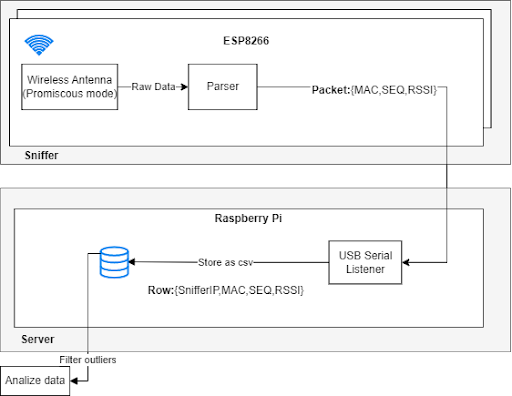
\includegraphics[width=0.7\textwidth]{Figuras/infraestructure/arduino-rpi.png}
	\captionsetup{margin=2cm}
	\caption[Flujo de datos en mediciones de perfilado]{Flujo de datos en mediciones de perfilado. El Arduino transfiere los datos mientras llegan directamente a la \acs{rpi} mediante \acs{usb}. Estos se agrupan por distancia (ingresada por el usuario) gracias al script de captura.}
	\label{fig:infra-diagram-arduino}
\end{figure}
\begin{figure}[!htb]
	\centering
	\includegraphics[width=0.8\textwidth]{Figuras/fieldwork/profiling-setup.png}
	\captionsetup{margin=2cm}
	\caption[Perfilado]{Experimento de campo de perfilado. Para que todos los dispositivos tengan sus antenas orientadas en el
mismo ángulo hacia la misma ubicación durante todo el experimento se utilizó
un soporte de metal con monturas hechas con impresora 3D.}
	\label{fig:arduino-profiling-setup}
\end{figure}

Antes de avanzar con los experimentos de campo hacia la etapa de multilateración, se quiso confirmar primero que la relación \acs{rssi} a distancia que informaban los \acs{esp} se acercaba a la realidad (es decir que se aproxime a lo que debería ser el ideal, o el modelo de \textit{Path Loss} antes visto). Similar a lo realizado en el experimento simulado pero con más nodos \textbf{Sniffer} para garantizar precisión.

Si bien se eligió utilizar una infraestructura \textit{wireless} más adelante como se describe en la sección \ref{sssec:num1}, primero se realizó un experimento preliminar cableado conectando tres \acs{esp} mediante \acs{usb} a una computadora \acl{rpi} para tomar múltiples muestras a una distancia conocida y poder poner un corte entre muestra y muestra a medida se recibíamos. De esta manera poder etiquetar múltiples muestras a 2 metros, a 5, a 10, etc.

Para recibir esta información se desarrolló un \href{https://github.com/agusalex/PacketSnifferServer}{script} que toma \textbf{M} muestras y luego se detiene a esperar a que el usuario le indique la nueva distancia en la que se realizará la próxima medición. De esta manera se obtiene \textbf{M} muestras agrupadas por la distancia, a esto le llamamos “\textit{step}”.


Además se decidió hacer el experimento de perfilado en un ambiente controlado (en el campo de deportes de la \acs{ungs} con muy poca interferencia en la banda 2.4 GHz). Se garantizó la precisión de los datos mediante la toma de 200 muestras por cada “\textit{step}” de medición. Y se realizaron 21 mediciones por cada dispositivo a 4.5 metros de distancia entre cada una. Dos de los dispositivos finalizaron el experimento, pero uno sufrió un desperfecto y dejó de recibir.
 
\begin{figure}[!htb]
	\centering
	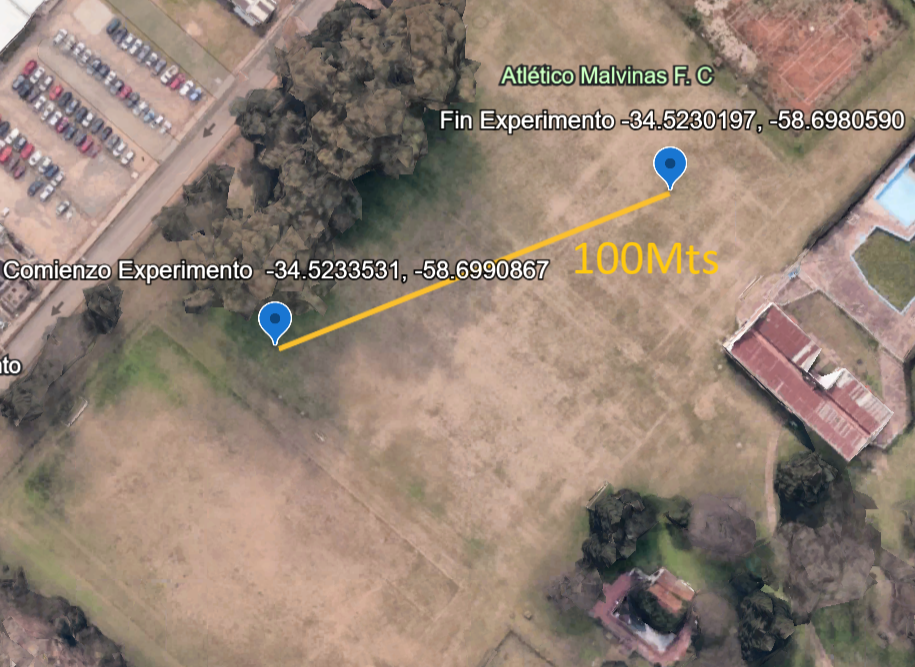
\includegraphics{Figuras/fieldwork/profiling.png}
	\captionsetup{margin=2cm}
	\caption[Perfilado]{Experimento de perfilado en el campo de deportes de la UNGS}
	\label{fig:arduino-profiling-setup}
\end{figure}
 Como transmisor se utilizó un dispositivo móvil en modo \acs{ap} para poder obtener una visión precisa del comportamiento de la señal.

Para procesar los datos de \acs{rssi}, primero se realizó un filtrado \textit{Kalman} de la captura entera por dispositivo, como se puede observar en la figura \ref{fig:filtrado-kalman}. Como último paso, calculamos la media por cada “\textit{step}” de distancia para filtrar las anomalías de los datos. Finalmente se ejecutó una regresión logarítmica usando cuadrados mínimos, el resultado nos da un \textbf{A} y un \textbf{N} que podría ser utilizado en el paso de multilateración.

\subsection{Experimento}
%\begin{figure}[!htb]
%	\centering
%	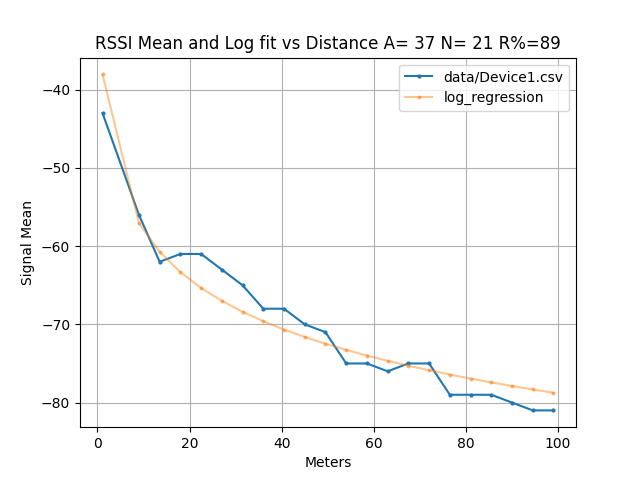
\includegraphics[width=0.8\textwidth]{Figuras/profiling/device1/device1_regression.png}
%	\captionsetup{margin=2cm}
%	\caption[Media de \acs{rssi} segregado por distancia de la medición vs regresión logarítmica, prueba de campo]{Media de \acs{rssi} segregado por distancia de la medición vs regresión logarítmica, prueba de campo con \textit{steps}”, con ESP8266 en campo de deportes UNGS. Se hallaron valores para \textbf{A=37}, \textbf{N=21} y \textbf{R(residual)=89\ }}
%	\label{fig:dev1-regression}
%\end{figure}

La figura \ref{fig:dev2-dev1-regression} muestra los resultados obtenidos de este experimento de campo. En el eje X se puede observar la distancia real desde el dispositivo \acs{esp} hasta el dispositivo móvil transmisor en metros, mientras que en el eje Y se representa el RSSI medido. Cada punto en el gráfico representa una medición individual del \acs{rssi} en una determinada distancia.



\subsection{Conclusión}

Puede observarse que a medida que la distancia aumenta, el \acs{rssi} se ajusta a una curva según lo predicho por el modelo, lo que se alinea con lo que esperaríamos de la pérdida de señal en función de la distancia en un entorno con mínima interferencia. Sin embargo, también se pueden identificar algunas variaciones y anomalías en los datos, posiblemente debido a factores ambientales no controlados o a variaciones inherentes en la recepción de la señal.
\begin{figure}
	\centering
	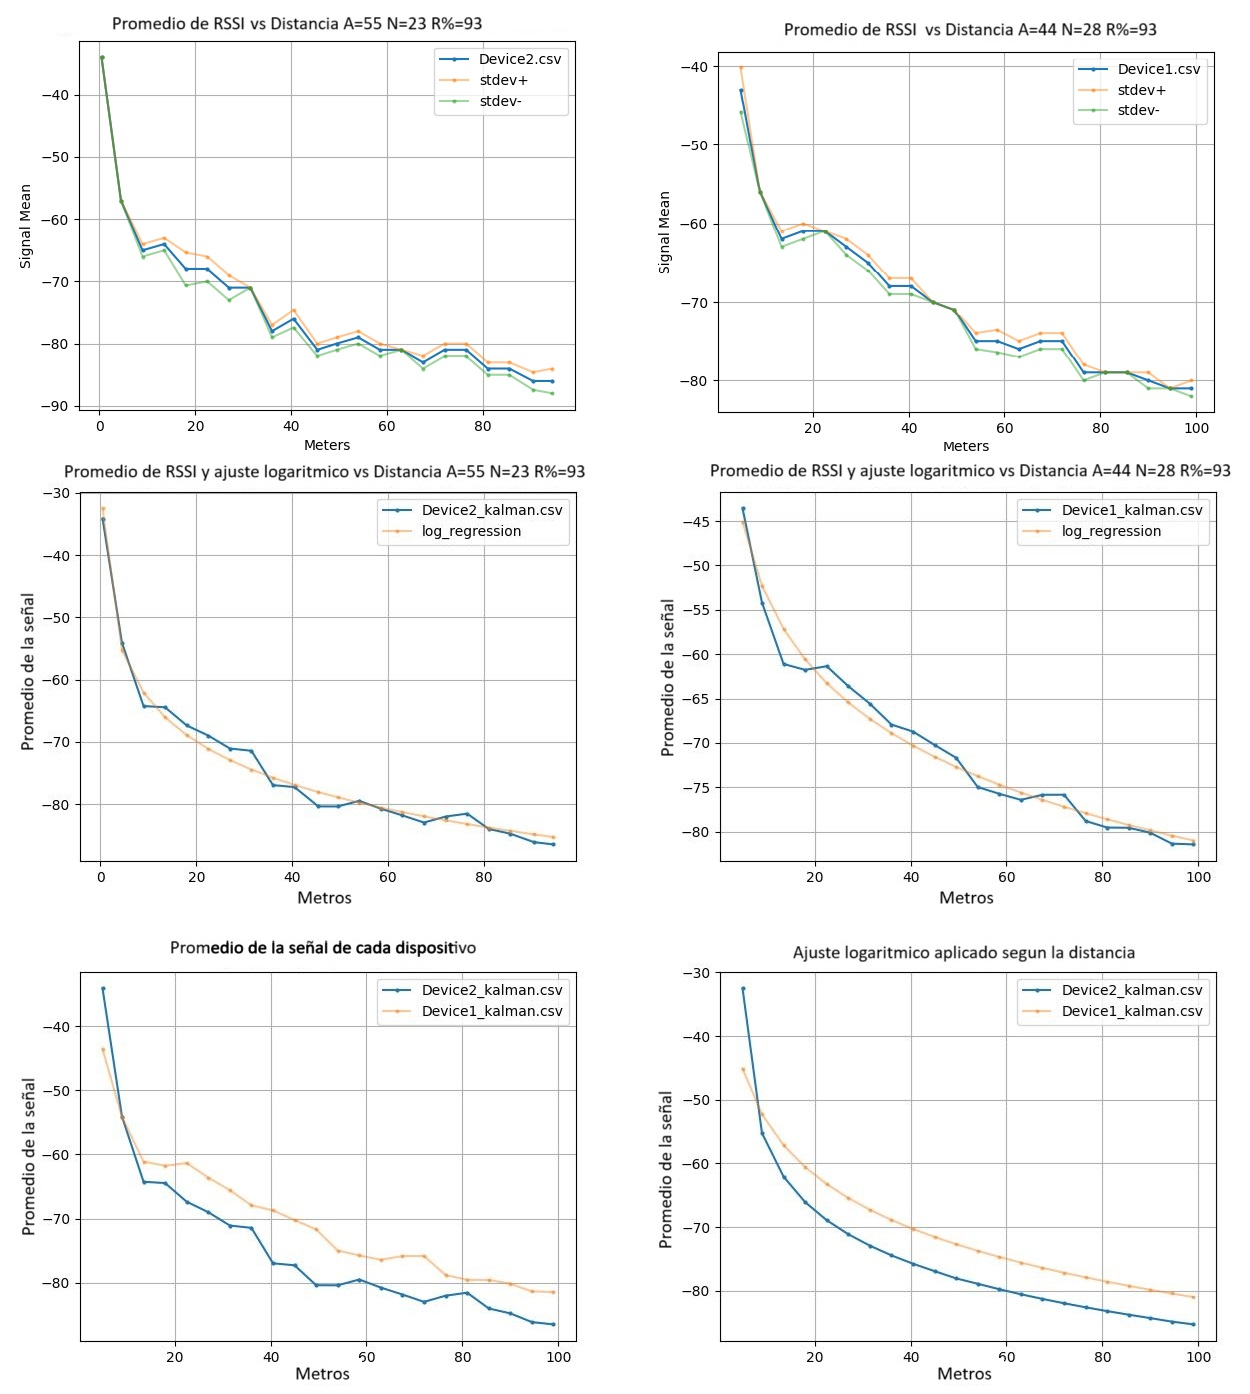
\includegraphics[width=1\textwidth]{Figuras/profiling/preliminar-experiment.jpg}
	\captionsetup{margin=2cm}
	\caption[Media de \acs{rssi} segregado por distancia de la medición vs regresión logarítmica, prueba de campo]{Media de \acs{rssi} segregado por distancia de la medición vs regresión logarítmica, prueba de campo con “\textit{steps}”, con ESP8266 en campo de deportes UNGS. Se hallaron valores del dispositivo 1 para \textbf{A=37}, \textbf{N=21} y \textbf{R(residual)=89}
    Para el dispositivo 2 \textbf{A=49}, \textbf{N=18} y \textbf{R(residual)=88}}
\label{fig:dev2-dev1-regression}
\end{figure}
Finalmente, realizamos una regresión logarítmica para obtener una representación ajustada de la relación entre la distancia y el \acs{rssi}. El resultado de esta regresión nos proporcionó los parámetros \textbf{A} y \textbf{N} para cada dispositivo, al igual que en el experimento simulado.




\section{Infraestructura de pruebas de campo \textit{wireless}} \label{sssec:num1}

\begin{figure}[!htb]
	\centering
	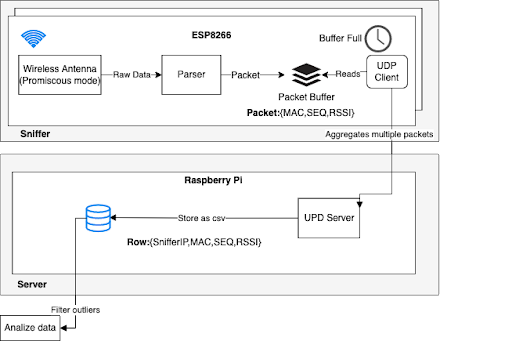
\includegraphics[width=0.8\textwidth]{Figuras/infraestructure/arduino-rpi-multi.png}
	\captionsetup{margin=2cm}
	\caption[Flujo de datos en mediciones de multilateración]{Flujo de datos en mediciones de multilateración. Los Arduinos recolectan los datos hasta agotar el espacio en memoria o llegar a un límite establecido. Finalmente descargan toda la información en una \acs{rpi} de manera inalámbrica.}
	\label{fig:infra-diagram-arduino}
\end{figure}

Se plantearon distintas alternativas de \textit{hardware} para poder cubrir el área más grande posible al menor costo. Se pensó en la utilización de \textit{routers} comerciales como los \textit{Ubiquiti} usando un software de código abierto como \textit{OpenWRT}, también la posibilidad de usar \acl{rpi} o similares e incluso microcontroladores con \acs{wifi} compatibles con Arduino como el \acs{esp} y el \acs{esp32}.

Cualquiera de estas soluciones trae consigo un problema ineludible: Los adaptadores \acs{wifi} hasta donde hemos podido investigar no pueden operar en modo promiscuo en simultáneo mientras que opera en otro modo, por ejemplo, en modo \acl{ap} o modo cliente mientras se encuentra en modo promiscuo. Se planteó la posibilidad de usar dispositivos que cuentan con dos adaptadores de \acs{wifi}, uno para capturar paquetes \acl{prq} y otro para evacuarlos hacia una base de datos centralizada para que luego puedan ser analizados pero no se encontró ninguno de bajo costo y de uso masivo.

Por esto fue elegida la alternativa de utilizar muchos dispositivos \acs{esp} como \textit{Sniffer} y un \textit{\acl{rpi} 3} en modo \textit{Access Point} para recibir los datos. Para facilitar las mediciones a modo de soporte aseguramos cada \textit{Sniffer} a un tubo de PVC con una base de cemento. Los \acs{esp} fueron adheridos con \textit{velcro} al tubo y se le agregó una batería de LI-ION conectada a los pines \acs{vin} y \acs{gnd} del dispositivo como se puede observar en la imagen \ref{fig:infra-diagram-arduino}.

El \acs{esp} fue programado utilizando Arduino y Platformio para el sensor y Python para el server que recibe los datos. Se configuró el dispositivo en modo promiscuo y se procedió a capturar paquetes y descomponer los \textit{Beacon Frames} en sus parámetros utilizando el \textit{SDK} del \acs{esp}. De dicho \textit{frame}, parte del 802.11, se extrae puntualmente el \acs{rssi}, \acs{mac} y el número de secuencia del paquete.

Se configuró el \acs{esp} para conectarse a una red Wi-Fi emitida por una \textit{\acl{rpi}} (configurada en modo \textit{AP} para facilitarnos la infraestructura de red) y enviar a la \acl{rpi} vía \acs{udp} los paquetes agregados de a grupos de \textbf{N} paquetes donde \textbf{N} es el máximo número que se podía enviar sin llenar el \textit{frame} de \acs{udp}. De esta manera optimizamos el tiempo de envío ya que múltiples nodos enviando a la vez de a un paquete pequeño por vez vía \acs{wifi} tendían a sobrecargar a la red y a la \acs{rpi} que necesita procesar y escribir los datos en una tarjeta SD.
La \textit{\acl{rpi}} contenía un script que recibe los datos \acs{udp} de cada nodo, y guarda en un solo archivo CSV la siguiente información: \textbf{ip\_sniffer}, \textbf{rssi}, \textbf{num\_secuencia}. Luego ese archivo se descarga manualmente conectándose por SSH a la \acs{rpi}.

El número de secuencia se emplea como un identificador único para cada paquete, permitiendo su agrupación durante la realización de experimentos de multilateración o perfilado, similar a cómo se agruparon los paquetes por milisegundos de captura en los experimentos simulados. Este método elimina la necesidad de mantener relojes sincronizados entre los nodos, como sería necesario si se usaran los milisegundos de captura como criterio de agrupación. Sincronizar relojes en un entorno de infraestructura \textit{wireless} representaría un desafío considerable que se decidió evitar.
De esta manera, al analizar un paquete, podemos identificarlo con certeza y comparar de manera inequívoca los \acs{rssi} recibidos y la diferencia entre estos para cada \textit{Sniffer}.

Finalmente, una vez capturadas suficientes tuplas de (\textbf{número\_secuencia}, \textbf{rssi}) descartando las que no sean de la \acs{mac} de nuestro \textit{Objetivo}, los dispositivos cortan la recepción antes de llenar la limitada memoria del dispositivo, este proceso suele durar 2 minutos aunque varía según la tasa de transmisión de paquetes del \textit{Objetivo}. Luego los \acs{esp} proceden a agregar las tuplas capturadas y enviarlas de a grupos mediante \acs{udp} hacia la \acs{rpi}. Esta última recopila los datos y les agrega la \acs{ip} de cada \textit{Sniffer} para poder identificar de dónde vino la información para luego ser procesada. Finalmente se persiste en un archivo CSV.

Como nodo \textit{Objetivo} se utilizó un teléfono celular en modo \acl{ap} para incrementar la tasa de transmisión de paquetes. De esta manera nos limitamos a capturar los paquetes de tipo \textit{Beacon Frame} que emite el teléfono usando su \acs{mac} como filtro. Consideramos que es un buen equivalente a una situación donde un transeúnte cuenta con un teléfono sin estar en modo \acl{ap} pero emitiendo \acl{prq}. Esto, con la salvedad de la Mac Address Randomization y la escasa frecuencia de emisión de los \acl{prq}, lo que no lo haría beneficioso para este experimento.

\section{Interferencias y Rango Usable para Multilateración con ESP8266}
\begin{figure}[!htb]
	\centering
	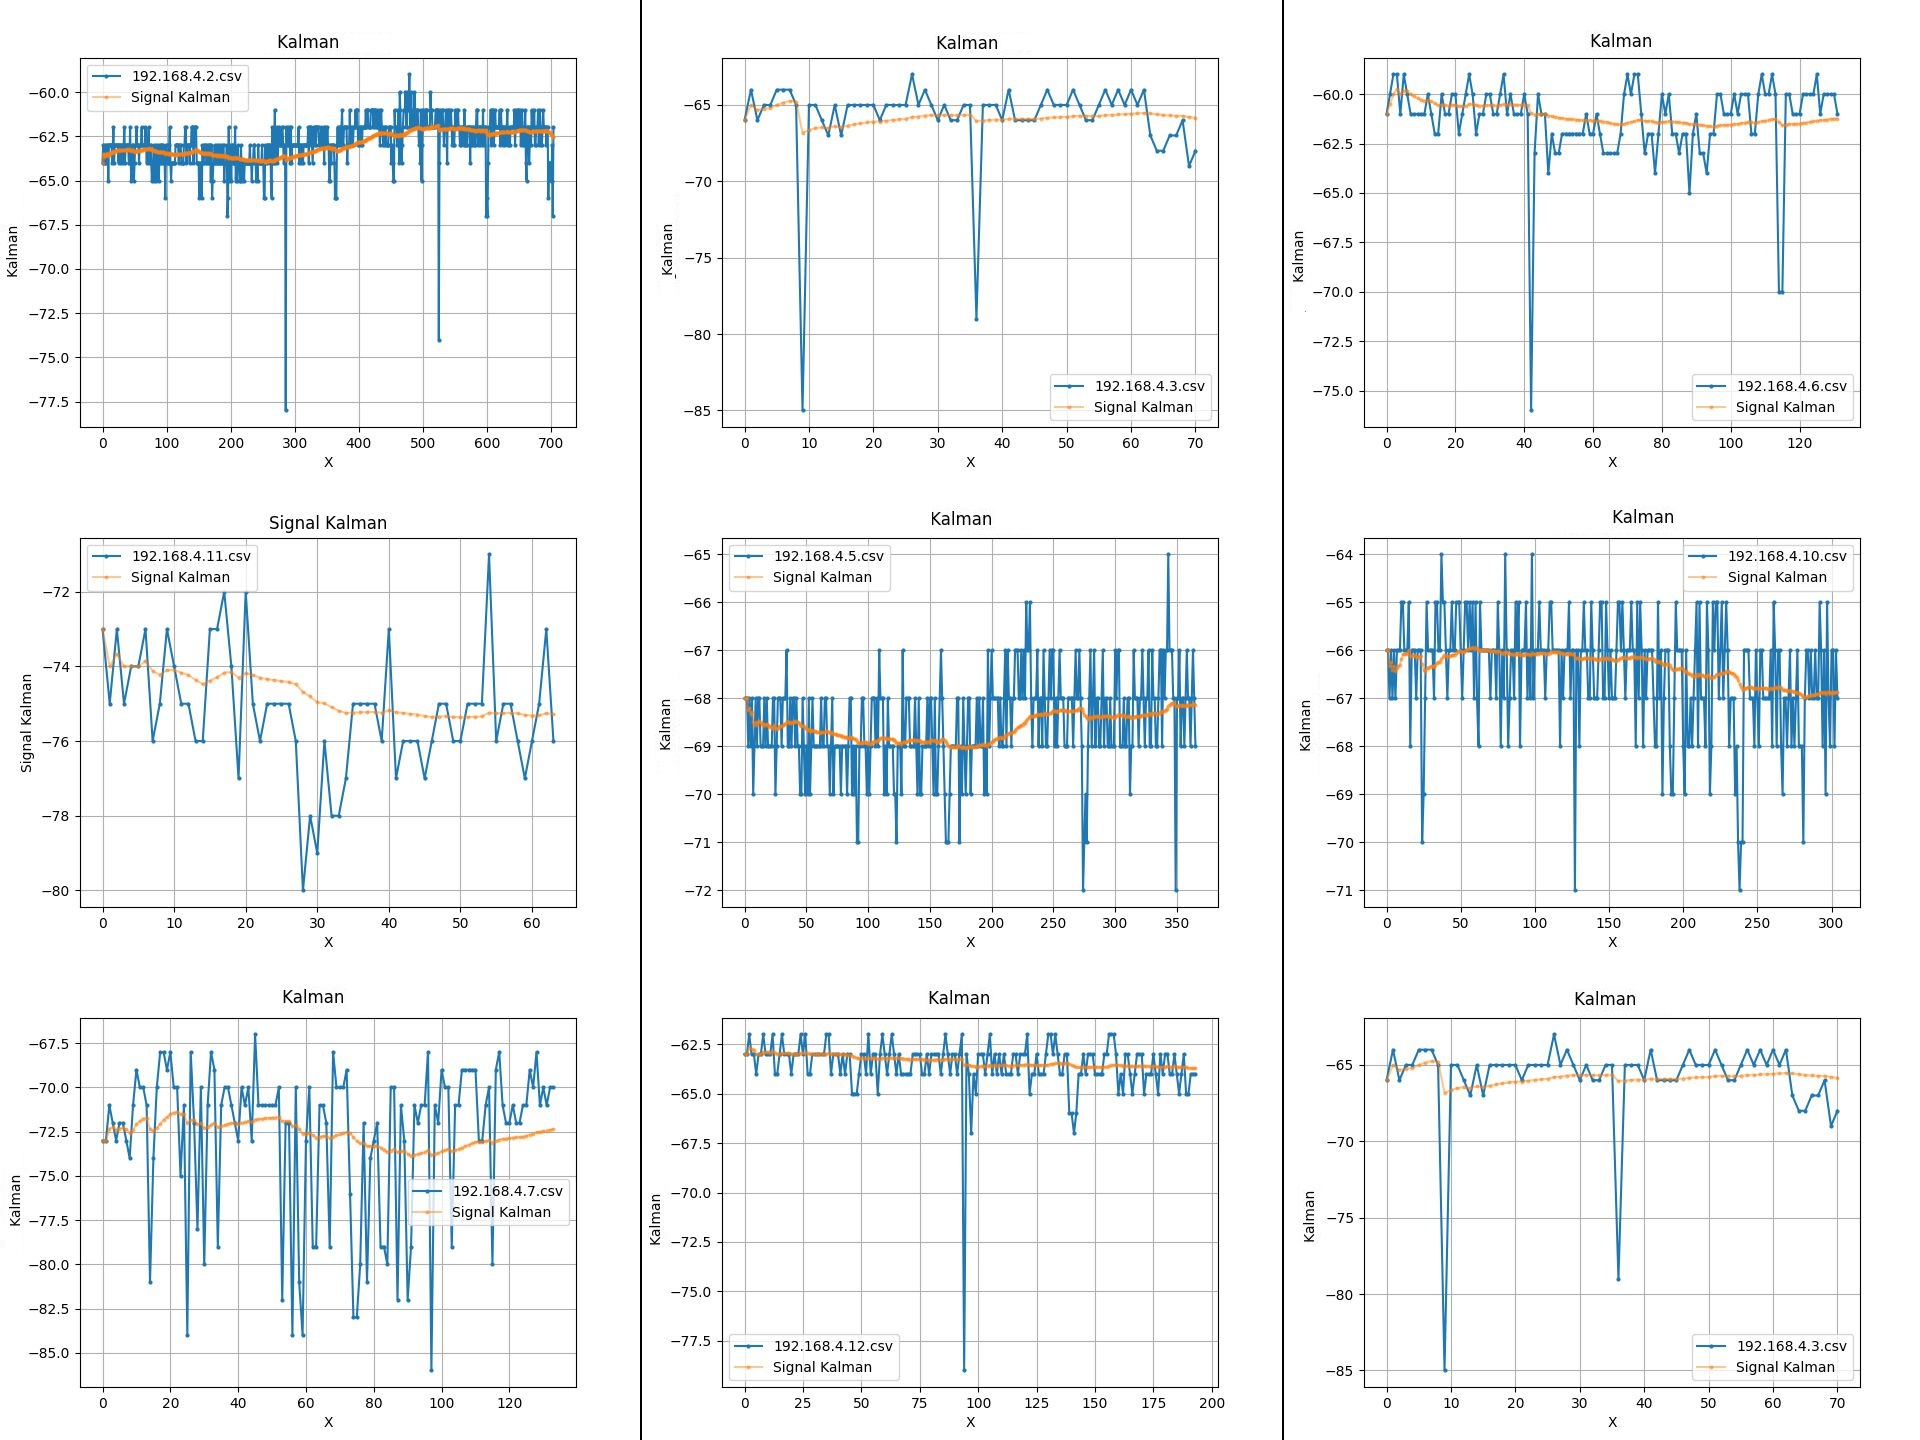
\includegraphics[width=0.95\textwidth]{Figuras/errores/estatico-medio.jpg}
	\captionsetup{margin=1cm}
	\caption[ Experimento estático]{ Experimento estático, misma disposición de nodos que el de multilateración. Se pueden observar grandes variaciones por interferencia del ambiente en el experimento sin movimiento. Los filtros de Kalman ayudan a mejorar esto.}
	\label{fig:errores-estatico}
\end{figure}
\subsection{Experimento estático}

 Utilizando la técnica de captura \textit{stepless} ya descrita se colocó un teléfono móvil a 15 metros de los nodos, los cuales se dispusieron en línea recta uno al lado del otro al igual que en el experimento de perfilado.
 Luego, sin mover el móvil, se procedió a capturar paquetes hasta completar la medición.
 Como se puede observar en la figura \ref{fig:errores-estatico} algunos nodos capturaron más datos que otros. Esto se debe a que durante la medición algunos nodos experimentaron fallos intermitentes en la alimentación, lo que provocó interrupciones en la recepción de señal. Durante la medición, algunos nodos experimentaron fallos intermitentes en la alimentación debido a un suministro de voltaje inadecuado. Esto ocurrió porque los nodos fueron alimentados directamente desde una batería de iones de litio con un voltaje nominal de 3.7V y un máximo de 4.2V, lo cual es insuficiente para el regulador AMS1117-3.3 integrado en la placa. Este regulador requiere un mínimo de 4.5V para operar correctamente; al no recibir un voltaje adecuado, la tensión de salida fluctuó por debajo de los 3.3V requeridos por el ESP8266, provocando estados inestables en su ejecución. Como resultado, algunos nodos dejaron de recibir paquetes al quedar en un estado de bloqueo (\textit{hang state}) o reiniciarse inesperadamente. Este problema afectó la consistencia de la captura de datos, generando discrepancias en la cantidad de paquetes registrados por cada nodo.

Otros experimentaron grandes interferencias, variando así por varios metros una potencial predicción de distancia.

 En todas las gráficas se puede ver cómo el filtro de Kalman ayuda a reducir el ruido y se adapta a los cambios en el perfil de recepción de la señal que persisten en el tiempo.
 Dicho filtro resultará una herramienta fundamental para mejorar la precisión en los experimentos subsiguientes.

\subsection{Precisión en el perfilado}


Luego de realizar varios experimentos de perfilado quedó en evidencia el problema que surge del modelo de \textit{Path Loss}: A medida que la distancia aumenta, la precisión baja considerablemente. Esto se puede observar en la figura \ref{fig:distance-error-range}, donde en la gráfica de la izquierda podemos observar cómo dada una posible interferencia temporal en la medición, la media de \acs{rssi} recibida a 12.5 metros es igual a la predicha por el ajuste logarítmico a 19 metros, en total un error de 6.5 metros. Lo que es más aún, la media de \acs{rssi} a 12.5 metros es igual a la media recibida a aproximadamente 25 metros, en total un error de 12.5 metros. Claramente, incluso a cortas distancias de menos de 20 metros se pueden ver distorsiones enormes en la distancia predicha. Continuando con este análisis, si consideramos la gráfica derecha en la misma figura, la cota inferior del desvío estándar (stdev-) a 27 metros es igual a la cota superior del desvío a 51 metros, en total, 24 metros de error entre ambos desvíos.

\begin{figure}[!htb]
	\centering
	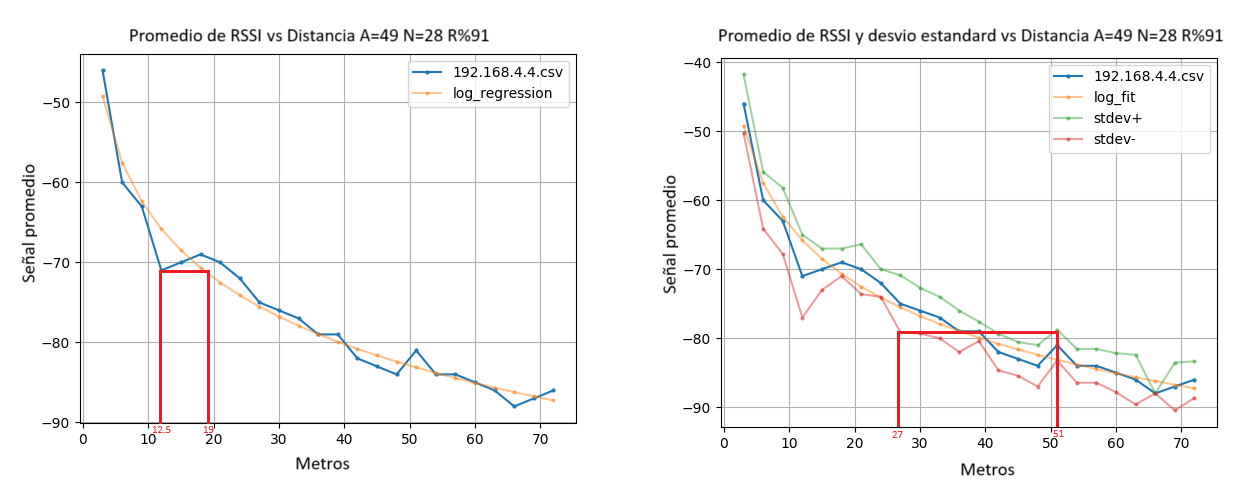
\includegraphics[width=0.95\textwidth]{Figuras/errores/4-raw-compilation-annotated.png}
	\captionsetup{margin=1cm}
	\caption[Variación de la distancia con \acs{rssi}]{Variaciones en la media y los desvíos estándar demuestran la poca precisión de estos dispositivos en distancias de más de 10 metros.}
	\label{fig:distance-error-range}
\end{figure}
\begin{figure}[!htb]
	\centering
	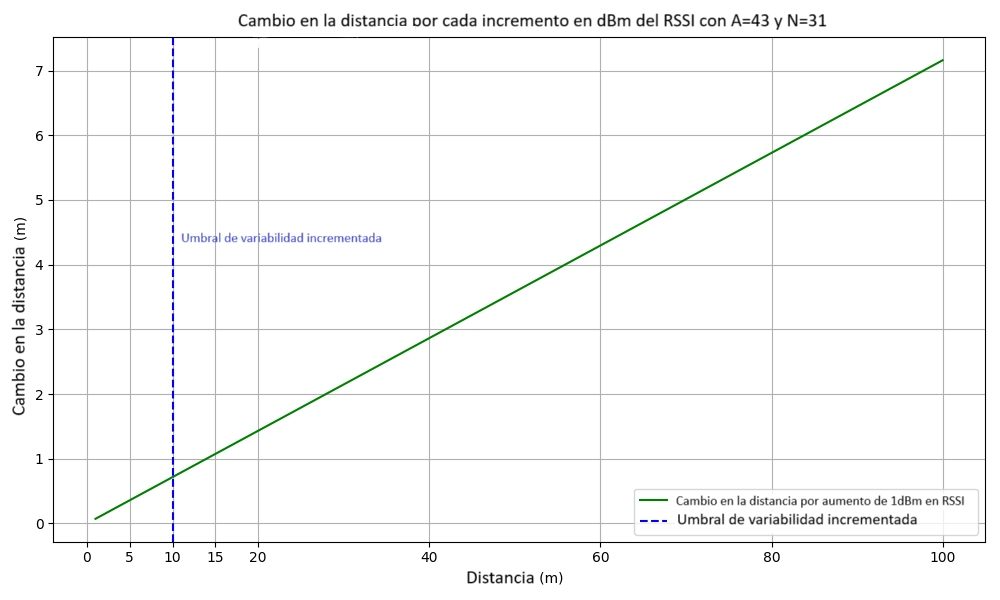
\includegraphics[width=0.95\textwidth]{Figuras/errores/distance_percentage_increase.png}
	\captionsetup{margin=1cm}
	\caption[Variación de la distancia con \acs{rssi}]{Variación de la distancia estimada por cada incremento de 1 dBm en \acs{rssi}, demostrando la precisión dentro de un rango de 10 metros y la creciente inexactitud más allá de este límite.}
	\label{fig:distance-percentage-increase}
\end{figure}

Por estos motivos se determinó que el rango usable efectivo de los dispositivos \acs{esp}, para experimentos de multilateración enfocados en identificar patrones de movimiento, es de hasta 10 metros. Incluso si se toma el modelo de \textit{Path Loss} sin interferencia como referencia, como podemos ver en la figura \ref{fig:distance-percentage-increase}, podemos observar que a partir de los 10 metros, por cada 1 dBm de variación en la intensidad de la señal \acs{rssi} se traducirá en cambios de aproximadamente 1 metro en la distancia estimada.

Este rango se ha demostrado adecuado para experimentos donde se buscaba determinar patrones de movimiento específicos, como patrones en forma de estrella o cuadrados, dentro de áreas confinadas. La elección de limitar las pruebas a una cuadrícula de 10x10 metros surgió tras experimentos multilaterales fallidos en áreas más extensas, como cuadrículas de 25x25 metros, donde el aumento de la imprecisión en las estimaciones de distancia comprometía la fiabilidad de los resultados.

Sin embargo, es importante destacar que el rango usable de 10 metros identificado en nuestra investigación es específico, primero, para el perfil de recepción de estos dispositivos y, segundo, puntualmente para la detección de patrones de movimiento detallados mediante multilateración. Para otros objetivos, como detección de presencia en áreas más amplias, el rango usable podría extenderse aún más. Y si consideramos el uso de antenas de mayor ganancia o la implementación de una mayor cantidad de dispositivos para cubrir un área mayor, este rango podría ser aún mejor.


\section{Perfilado sin \textbf{\textit{steps}}}

A pesar de los resultados prometedores obtenidos en los experimentos preliminares de perfilado, se hizo evidente que el perfilado es específico para cada sensor en un ambiente determinado. Esto se debe a que la curva de atenuación de la señal, que describe cómo disminuye la intensidad de la señal a medida que el transmisor se aleja, depende en gran medida del ruido ambiental del lugar donde se realice el experimento y de las características propias de cada dispositivo.

\begin{figure}[!htb]
    \centering
    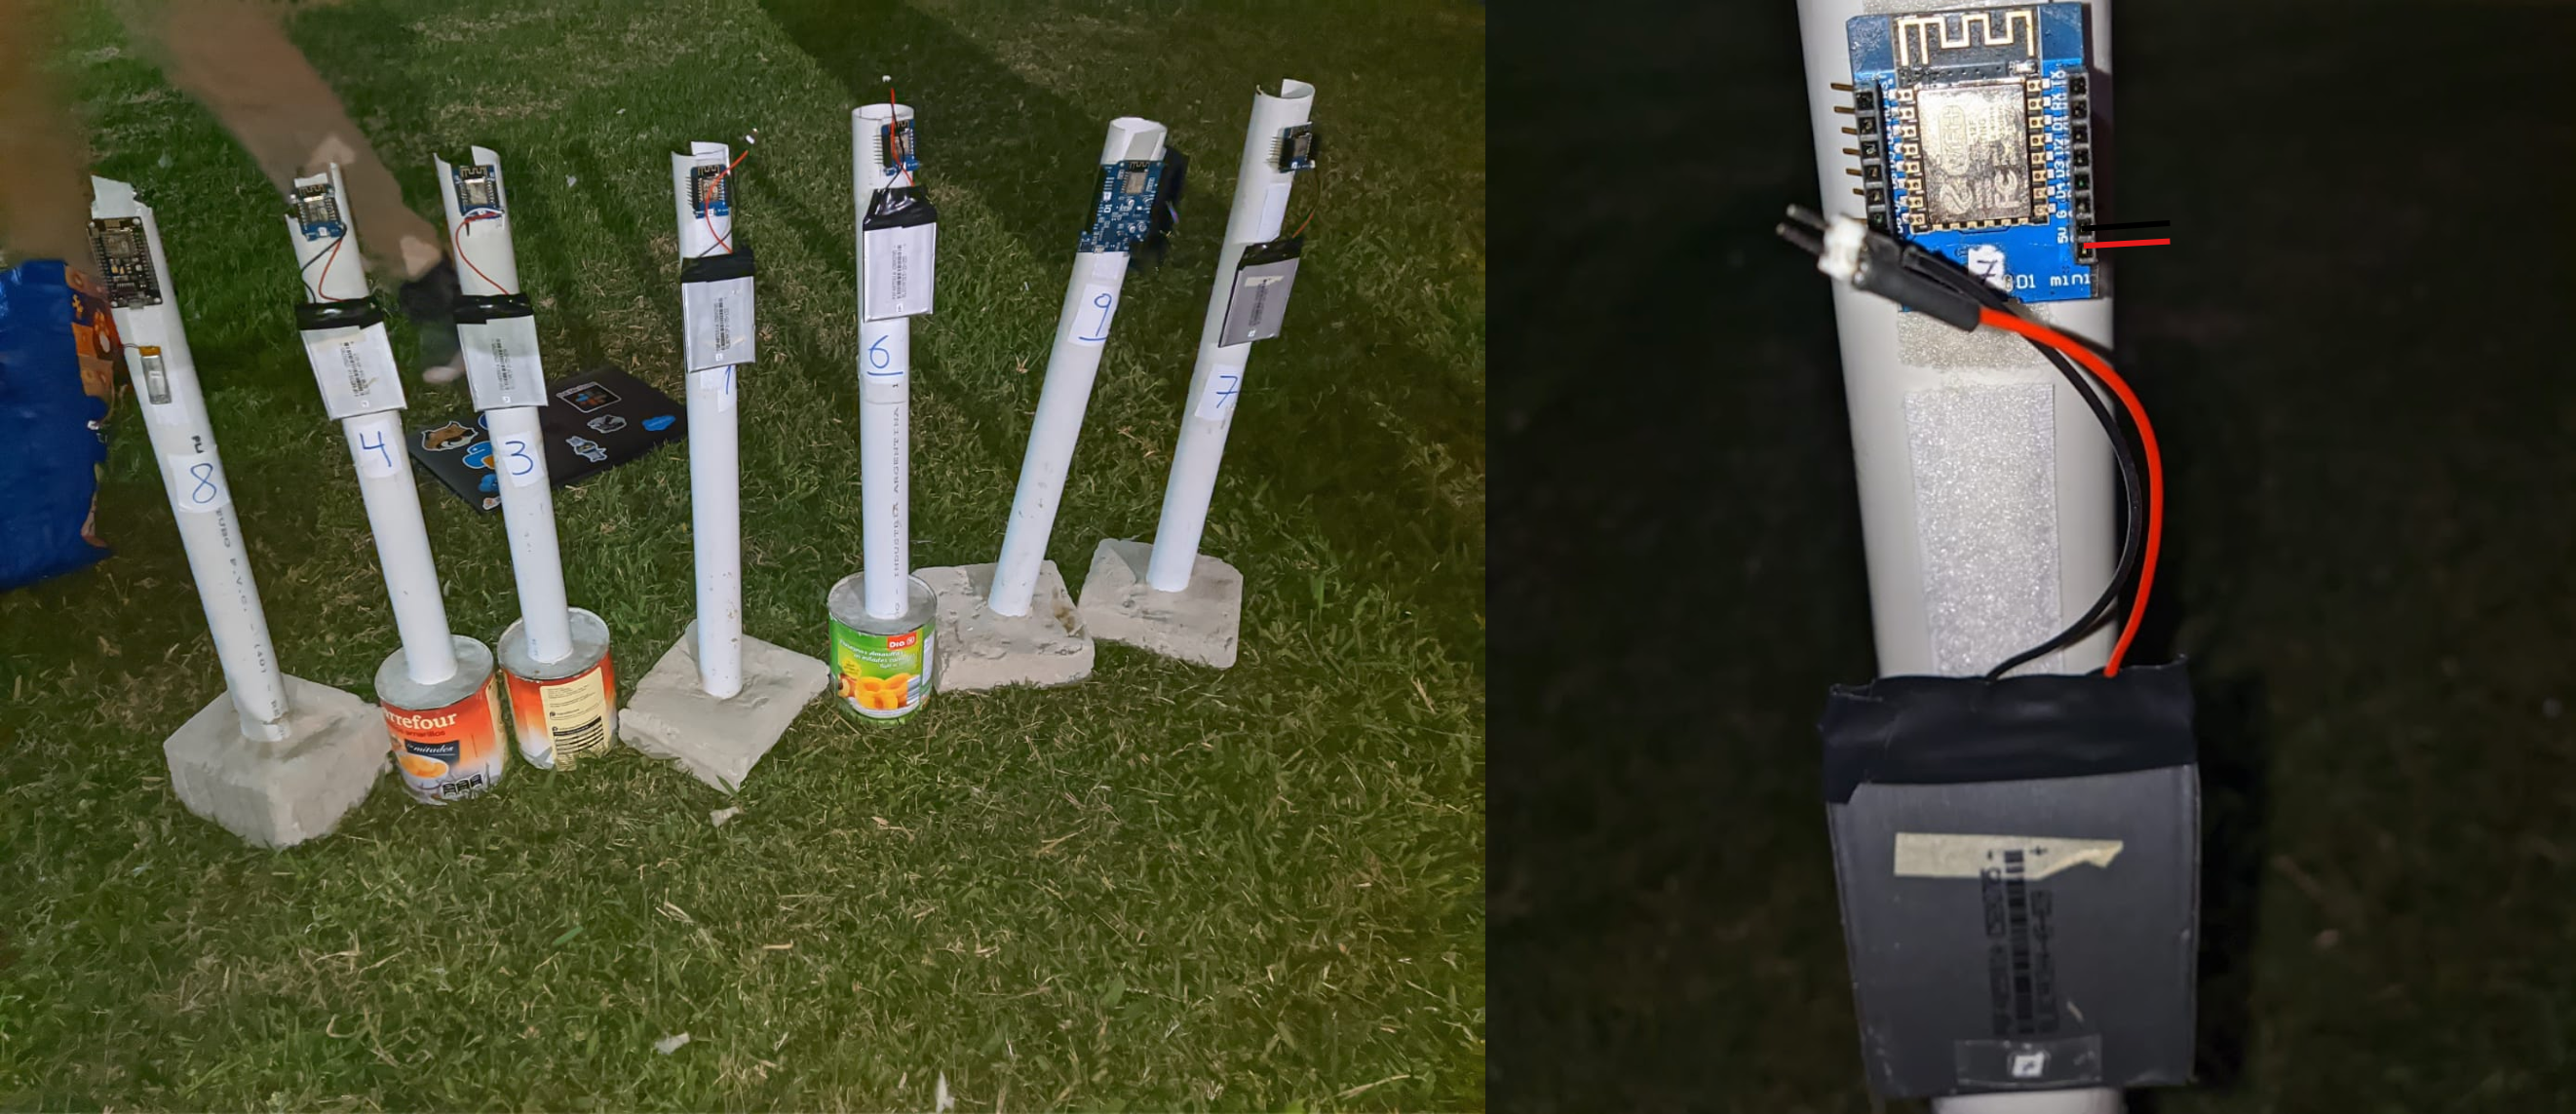
\includegraphics[width=0.8\textwidth]{Figuras/fieldwork/combined.png}
    \captionsetup{margin=2cm}
    \caption[Postes de Nodo Multilateración]{A la izquierda: Nodos \textit{Sniffer} construidos con PVC y una base de cemento. El ESP8266 fue adherido con velcro al tubo junto con una batería de LI-ION. A la derecha, un acercamiento a uno de los nodos notando donde se conectó el ESP8266 a la batería utilizando los terminales 5V y GND.}
    \label{fig:infra-diagram-arduino}
\end{figure}
Con el objetivo de evaluar la capacidad para predecir movimientos de un individuo en un ambiente urbano, y ante las limitaciones de acceso al campo de deportes de la \acs{ungs}, se optó por realizar experimentos en el campus de la \acs{ungs}, un lugar de alta concurrencia y con potencial interferencia de señal debido a la presencia de edificios. Del cual podíamos disponer en cualquier momento y así realizar más experimentos.

\begin{figure}[!htb]
    \centering
    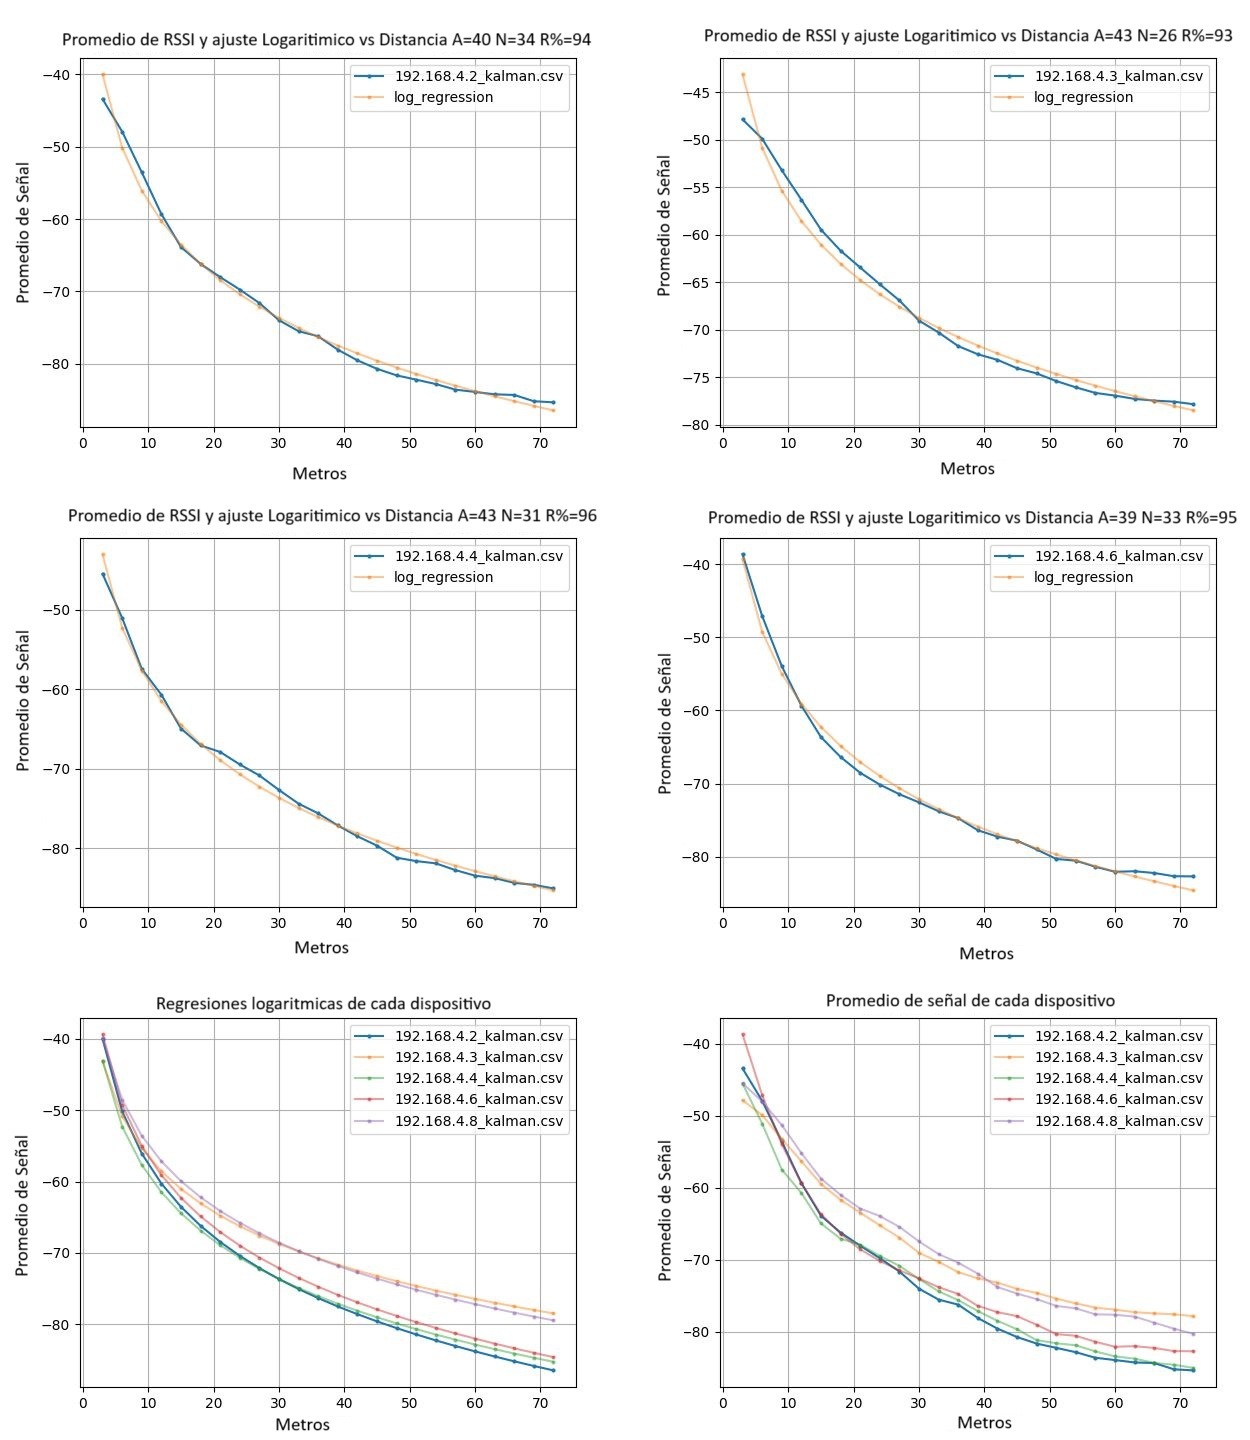
\includegraphics[width=0.95\textwidth]{Figuras/profiling/stepless.png}
    \captionsetup{margin=1cm}
    \caption[Stepless]{Resultados de perfilado \textit{stepless}.}
    \label{fig:stepless}
\end{figure}
Se decidió además probar el método de captura \textit{wireless} descrito en la sección \ref{sssec:num1} en un escenario de perfilado conocido antes de avanzar a la etapa de multilateración, con el fin de integrar todos los componentes de este trabajo. Este método no solo facilita la realización del experimento de perfilado, sino que también se asemeja más al escenario final de multilateración que se empleará posteriormente.

El término \textit{stepless} hace referencia a un enfoque de perfilado que no requiere de los pasos discretos predefinidos en términos de distancia conocida durante la captura de datos. En lugar de establecer intervalos fijos de distancia para la toma de mediciones, este método permite una captura continua a medida que el \textbf{Objetivo} se mueve a través del espacio. No obstante, para poder utilizar las ya mencionadas herramientas de perfilado, todavía se generan "pasos" virtuales basados en el tiempo y la secuencia de los paquetes capturados, lo que permite estimar la distancia recorrida. Estos pasos generados no corresponden a agrupaciones discretas con distancias conocidas, sino que son el resultado de una estimación que utiliza la secuencia de paquetes, la velocidad de movimiento y la frecuencia de transmisión del dispositivo móvil, facilitando así un análisis detallado sin la necesidad de mediciones de distancia fijas y conocidas previamente.

\subsection{Experimento}


A diferencia del experimento preliminar de perfilado realizado en el campo de deportes, este experimento se llevó a cabo en el campus de la UNGS.

Se dispusieron múltiples nodos en línea perpendicular al recorrido, formando una T con este, y se procedió a alejarse hasta alcanzar los 75 metros. Una vez completado el recorrido, se esperó a que los nodos finalizaran la captura y descarga de datos.

El método de captura \textit{wireless} empleado consiste en caminar a velocidad constante desde el punto donde se ubican los sensores, tomando nota del tiempo transcurrido hasta alcanzar una distancia determinada (por ejemplo, 30 metros en 30 segundos), mientras los sensores capturan los paquetes. Una vez finalizado el experimento, los datos se almacenan en la \acs{rpi}.

Dado que el dispositivo móvil utilizado (Samsung S20) emite paquetes cada 150 ms y conocemos el número de secuencia de cada paquete, es posible estimar la distancia a la que fue capturado y agruparlos en \textit{steps} discretos de distancia. Aunque se pierde precisión en la distancia exacta de captura, este agrupamiento y el cálculo del promedio mitigan el potencial error.

\subsection{Conclusiones}

El perfilado sin \textit{steps} permitió realizar experimentos de manera más rápida, facilitando la obtención de los valores de \(N\) y \(A\) en diferentes ambientes y para múltiples nodos simultáneamente, sin necesidad de conexión por cable o de tomar notas manuales sobre las distancias, reduciendo el tiempo de medición de 1 hora a 15 minutos. Además, se posiciona como una opción ideal para el despliegue rápido de nodos en un nuevo ambiente. Como se muestra en la figura \ref{fig:stepless}, se logró determinar los valores de \(N\) y \(A\) para cada sensor.

No obstante, algunos sensores presentaron interferencias significativas o su recepción se detuvo abruptamente, un problema recurrente a lo largo de este trabajo. La variabilidad observada en un experimento estático sin movimiento sugiere posibles defectos en los nodos o interferencias en el área de experimentación que afectaron a algunos nodos más que a otros, como se ilustra en la figura \ref{fig:errores-estatico-medio}.


\section{Multilateración}

\begin{figure}[!htb]
    \centering
    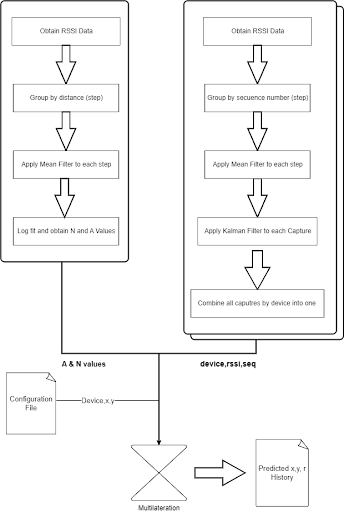
\includegraphics[width=0.6\textwidth]{Figuras/infraestructure/infra-diagram.png}
    \captionsetup{margin=2cm}
    \caption[Flujo de datos]{Flujo de datos en el experimento de multilateración.}
    \label{fig:infra-diagram}
\end{figure}
\begin{figure}[!htb]
	\centering
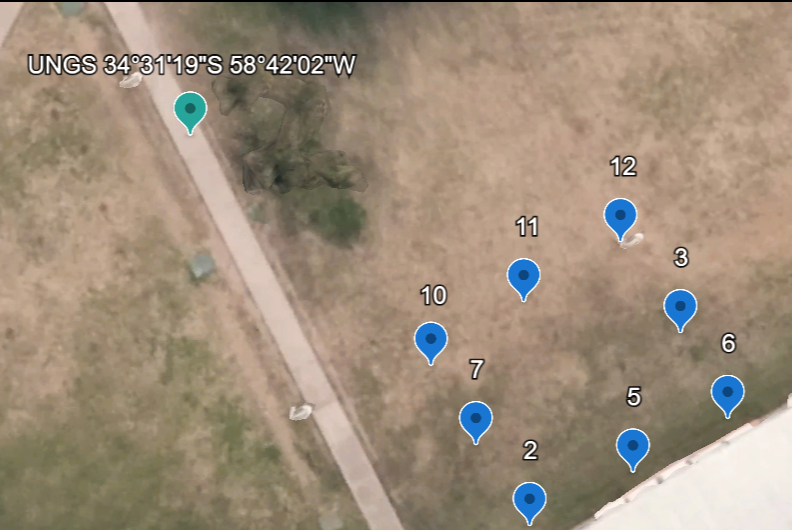
\includegraphics{Figuras/fieldwork/trilateration.png}
	\captionsetup{margin=2cm}
	\caption[Perfilado]{Experimento de perfilado en el campus de la UNGS}
	\label{fig:arduino-profiling-setup}
\end{figure}
\subsection{Infraestructura}

De manera similar al experimento de perfilado, se implementó una red de nodos \textbf{Sniffer} en el campus de la \acs{ungs}, siguiendo un esquema predeterminado. En este caso, se colocaron ocho nodos formando un cuadrado de 10 x 10 metros. Estos nodos se dedicaron a monitorear las señales Wi-Fi, capturando la intensidad de la señal \acs{rssi} emitida por el nodo \textbf{Objetivo}, que se desplazaba siguiendo una ruta preestablecida dentro del alcance de los nodos \textbf{Sniffer}. Durante el experimento, el nodo \textbf{Objetivo} mantuvo una velocidad constante.

Los nodos \textbf{Sniffer} registraron la \acs{rssi} de las señales emitidas por el nodo \textbf{Objetivo}, junto con el número de secuencia de cada señal, transmitiendo estos datos a una \acl{rpi} mediante Wi-Fi, una vez completado el experimento y llenados sus buffers para el posterior análisis de los datos.

Con los valores de \textbf{A} y \textbf{N} derivados de los experimentos de perfilado previos y utilizando la fórmula que convierte el valor de \acs{rssi} en distancia, se estimó la separación entre cada nodo \textbf{Sniffer} y el nodo \textbf{Objetivo} para cada paquete con el mismo número de secuencia. Se realizaron un mínimo de cinco mediciones de distancia con distintos nodos para cada punto en el tiempo para garantizar una mayor precisión.

Si bien durante la etapa de perfilado, se calculó un \textbf{A} y un \textbf{N} distintos para cada nodo. Tal como se discutirá más adelante, las interferencias fueron un factor muy importante durante las pruebas en el campus de la \acs{ungs}. Muchos nodos arrojaron valores muy distintos simplemente por los grandes cambios en la señal, incluso estando quietos, como se aprecia más adelante en la figura \ref{fig:errores-estatico}. Por este motivo, se eligieron los valores de \textbf{A} y de \textbf{N} del experimento de perfilado que mejor ajuste tuvo, es decir que tuvo menor residual.
En este caso \textbf{A=43} y \textbf{N=31}.

\begin{figure}[!htb]
\centering
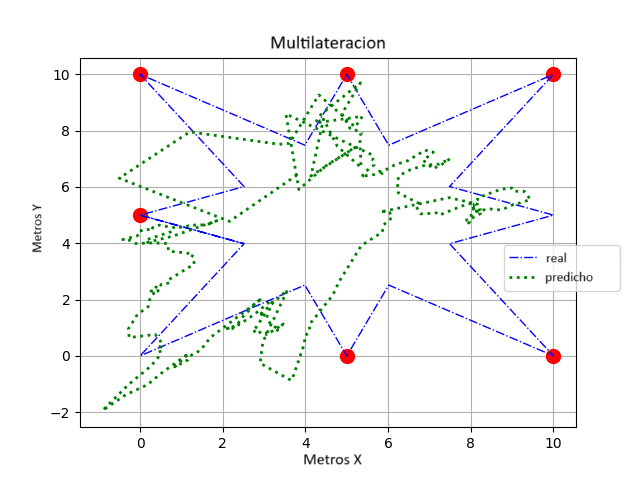
\includegraphics[width=0.8\textwidth]{Figuras/multilateration/multilateration_star.png}
\captionsetup{margin=2cm}
\caption[Configuración de la multilateración en Tiempo Real]{Configuración del experimento de multilateración en tiempo real en el campo de deportes de la \acs{ungs}.}
\label{fig:real-multilateration}
\end{figure}

\begin{figure}[!htb]
\centering
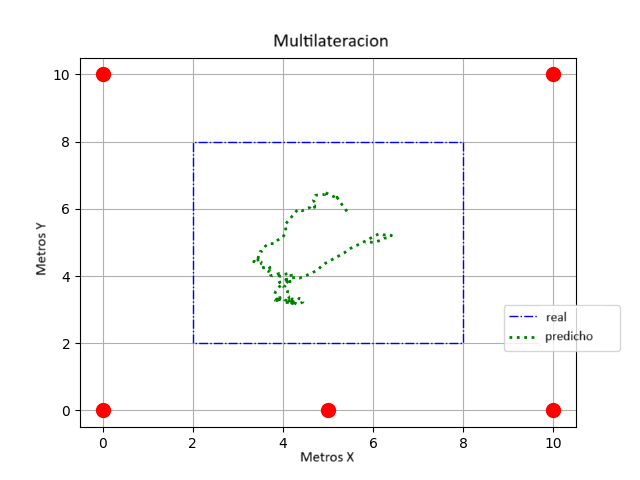
\includegraphics[width=0.8\textwidth]{Figuras/multilateration/multilateration_square.png}
\captionsetup{margin=2cm}
\caption[Resultados de la multilateración en Tiempo Real]{Resultados de la multilateración en tiempo real, mostrando la trayectoria estimada del nodo \textbf{Objetivo} en comparación con su trayectoria real.}
\label{fig:real-multilateration-results}
\end{figure}


\subsection{Experimento}

Se llevaron a cabo múltiples recorridos en distintas ejecuciones de este experimento. Si bien durante el experimento se utilizaron 8 nodos, en la figura \ref{fig:real-multilateration} solo se representaron con círculos rojos 6 nodos. En la figura \ref{fig:real-multilateration-results} se puede ver que solo hay representados 5 nodos. Esto se debe a que algunos nodos presentaron altas interferencias y sus datos fueron descartados. También se debe a que algunos nodos no recibieron señal parcial o totalmente en algunos o todos los experimentos. Estos fenómenos serán explicados en más detalle en el capítulo \ref{Cap_Errores}.
La multilateración se llevó a cabo comparando las posiciones estimadas del nodo \textbf{Objetivo} con su trayectoria real, con el fin de evaluar la precisión de este método. Aunque los resultados mostraron cierto nivel de error en la estimación de la ubicación, estos se discutirán en detalle en la sección siguiente.


Las estimaciones de la ubicación obtenidas mediante la multilateración, representadas en las figuras \ref{fig:real-multilateration} y \ref{fig:real-multilateration-results}, se compararon con la trayectoria real del nodo \textbf{Objetivo} para evaluar la precisión del método. En los gráficos, los nodos \textbf{Sniffer} están ubicados en posiciones fijas, mientras que el nodo \textbf{Objetivo} sigue una ruta predeterminada.

Cada punto en los gráficos simboliza una estimación de la posición del nodo \textbf{Objetivo}, calculada a partir de las mediciones de \acs{rssi} recogidas por varios nodos \textbf{Sniffer}, el número de secuencia de los paquetes, y los parámetros \textbf{A} y \textbf{N} obtenidos de los experimentos de perfilado.

La línea azul ilustra la trayectoria real seguida por el nodo \textbf{Objetivo}, mientras que la línea verde muestra las estimaciones de su posición según la multilateración. Se puede observar que las estimaciones recrean levemente la trayectoria original, aunque presentan grandes deformaciones.


\subsection{Conclusión}

A pesar de las discrepancias y deformaciones observadas en las estimaciones de la ubicación del nodo \textbf{Objetivo}, el recorrido estimado mantiene cierta semejanza con la trayectoria original. Esto indica que, aunque existen errores significativos en la precisión de la localización, el enfoque de multilateración empleado logra capturar la esencia del movimiento del nodo \textbf{Objetivo} dentro del área de cobertura de los nodos \textbf{Sniffer}. Sin embargo, se identificaron zonas donde las estimaciones se alejaban significativamente de la trayectoria real, atribuibles a diversos factores como la interferencia inalámbrica, movimientos no intencionados del nodo \textbf{Objetivo}, y errores en la medición de \acs{rssi}.

Dentro de los resultados obtenidos, las discrepancias constantes en las estimaciones de ubicación, manifestadas como desplazamientos constantes o rotaciones en el gráfico, pueden deberse a múltiples factores relacionados con el entorno y la metodología de medición. Un desplazamiento constante en las estimaciones indica un sesgo sistemático en la medición del \acs{rssi}, posiblemente a causa de diferencias en la ganancia de las antenas de los nodos \textbf{Sniffer} o que la antena del nodo \textbf{Objetivo} no fuera precisamente omnidireccional (como no suelen serlo en teléfonos móviles).

Por otro lado, las rotaciones observadas en la predicción del recorrido, podrían deberse a personas en el camino de la señal o errores en la ubicación de los nodos, por ejemplo, un velcro flojo y un nodo que apunta ligeramente hacia un lado o al otro. Factores adicionales, como la reflexión de señales en superficies cercanas o la difracción a través de obstáculos también pueden contribuir a los errores y deformaciones registrados.
%\chapter{Discusiones}
\label{Cap_Errores}
\label{Capitulo_5}

Los experimentos realizados, tanto en entornos simulados como reales, han mostrado resultados alentadores en la estimación de ubicación, mostrando resultados prometedores en la estimación de ubicación. Al mismo tiempo, se han detectado ciertos errores y limitaciones que afectan la precisión del sistema. En este capítulo analizaremos en detalle los errores identificados y propondremos mejoras que permitan optimizar aún más el desempeño de un sistema similar.


\section{Análisis de Errores y Mejoras}

\subsection{Interferencia Ambiental y Variabilidad de la Señal}

Uno de los principales desafíos encontrados durante los experimentos fue la interferencia ambiental, que afecta significativamente la calidad y la consistencia de las señales \acs{wifi}. Como se muestra en la Figura \ref{fig:errores-estatico}, las variaciones en la intensidad de la señal \acs{rssi} debido a la interferencia del ambiente pueden introducir errores significativos en la estimación de la distancia y, por ende, en la localización del dispositivo.

Otro impedimento fue la inconsistencia en la recepción de paquetes, atribuible a inestabilidades en el suministro de energía de los dispositivos utilizados. Como se puede ver también en la Figura \ref{fig:errores-estatico}, se observó una marcada diferencia en el número de muestras recibidas: mientras algunos dispositivos capturaron hasta 700 muestras, otros apenas 70. Dado que no hubo movimiento en el experimento, estas discrepancias sugieren que, además de la interferencia ambiental, la variabilidad en la alimentación al usar batería de \textit{LI-ION} sin adaptar el voltaje a 5V continuo pudo haber afectado el desempeño, generando fallos a nivel de hardware.

\textbf{Se propone como trabajo futuro:}
Primero revisar la consistencia en la recepción mejorando la alimentación del hardware agregándole un módulo \textit{Step-Up} de 3V-4V a 5V. Para mitigar el impacto de la interferencia ambiental, se recomienda implementar algoritmos de filtrado más avanzados, como filtros de partículas o técnicas de aprendizaje automático, que puedan identificar y compensar las fluctuaciones anómalas en la intensidad de la señal en tiempo real. Además, el uso de modelos de propagación de señales más complejos que tengan en cuenta las características específicas del entorno urbano puede ayudar a mejorar la precisión de las estimaciones.

\subsection{Desafíos en la Multilateración y la Estimación de Distancias}

La multilateración, aunque efectiva en teoría, se enfrenta a desafíos prácticos significativos cuando se implementa en entornos urbanos densamente poblados. La precisión de la multilateración depende de la exactitud de las estimaciones de distancia basadas en el \acs{rssi}, que pueden verse comprometidas por múltiples factores, incluyendo la orientación de los dispositivos y la presencia de obstáculos físicos.

\textbf{Se propone como trabajo futuro:}
Una posible mejora sería incorporar información adicional en el proceso de perfilado, mediante la adición de un módulo \acs{gps}. Se podrían, de esta manera, incorporar coordenadas exactas de los nodos durante la etapa de perfilado y la orientación exacta del dispositivo pasaría a ser irrelevante si se utiliza una antena omnidireccional. 

Otra mejora podría ser realizar perfilado individual por cada nodo y aplicar los valores encontrados en el proceso de multilateración. En vez del perfilado general realizado donde se eligieron los valores con el menor residual y se aplicaron a todos los nodos.

Finalmente, la calibración periódica de los nodos \textbf{Sniffer} utilizándose entre sí mismos como puntos conocidos permitiría el ajuste dinámico de los parámetros del modelo de propagación de señales contribuyendo así también a una mayor precisión.




\subsection{Limitaciones del Hardware y la Infraestructura}

El rendimiento y las capacidades de los nodos \textbf{Sniffer} basados en \acs{esp}, aunque impresionantes dada su baja coste y accesibilidad, imponen limitaciones en términos de procesamiento y alcance de la señal. Estas limitaciones pueden restringir la escala y la resolución de los experimentos de localización.


Desde que el grupo de investigación comenzó a utilizar los \acs{esp}, surgieron múltiples problemas. El más grave de ellos fue la confiabilidad en la recepción de señal. Hubieron experimentos enteros que tuvieron que ser descartados debido a la recepción de la señal con grandes errores. Y muchos donde uno o varios de los nodos por momentos dejaron de recibir señal. Si bien algunos de estos problemas fueron identificados como falta de energía por el error al conectar el suministro de 5V como se describió anteriormente, también se lo atribuimos al software. El ESP-SDK, que si bien nos facilitó poner dichos dispositivos en modo promiscuo, dificultó el desarrollo del trabajo. Durante los primeros experimentos los datos de dichas pruebas tuvieron que ser completamente descartados por haber usado como base para nuestro software ejemplos de código del SDK disponible en internet que emitía mediciones completamente erradas de \acs{rssi}. Luego se investigó un poco más y se utilizó otro software y fue resuelto. El software utilizado se encuentra en el último capítulo de este trabajo.

Los problemas observados en los experimentos se deben, en parte también, a la forma en que se instalaron los nodos. En la configuración actual, los nodos se apoyaron sobre un tubo de PVC, lo que implicó que quedaran orientados en direcciones desconocidas y utilizaban las antenas que vienen impresas en el circuito del dispositivo que sabemos que tienen un patrón direccional sesgado en lugar de antenas omnidireccionales \cite{Yoppy2018RSSICO}. Además, la ubicación GPS de los nodos fue estimada, lo que impidió conocer con exactitud su posición y altura. En un escenario ideal, al emplear antenas omnidireccionales la orientación de los nodos no afectaría la captación de señales y si se dispone 
de datos precisos de GPS, junto con una altura definida (por ejemplo, al estar instalados en postes de luz), permitiría obtener mediciones más estables y precisas.

Además La recepción de paquetes se vio limitada en su duración ya que la memoria de los dispositivos se llena muy rápido y al no tener múltiples interfaces, una para recibir y otra para transmitir los paquetes. Sólo era posible recibir y enviar por turnos debido a que en modo promiscuo sólo es posible recibir en esa interfaz.

\textbf{Se propone como trabajo futuro:} la exploración de hardware alternativo que incorpore múltiples antenas, una para la recolección de datos y otra para la evacuación, con capacidades superiores de procesamiento y una antena con mejor ganancia para mejorar la recepción de señales. Además, el desarrollo de una infraestructura de red robusta que permita manejar de manera eficiente la recopilación y el análisis de grandes volúmenes de datos de \acs{rssi} para ser enviados a un servidor centralizado, será fundamental para superar las limitaciones actuales. Estas mejoras permitirían que los nodos se mantuvieran más fijos y que las mediciones fueran más precisas, optimizando el desempeño en aplicaciones a gran escala.

\section{Consideraciones Finales}
Durante el análisis de errores se constató que, si bien la localización y seguimiento de dispositivos móviles en entornos urbanos presenta desafíos inherentes, los experimentos han permitido identificar áreas claras de mejora. Las estrategias de optimización implementadas han contribuido a mejorar la consistencia en la recepción de señales y la precisión de las estimaciones, lo que refuerza la viabilidad del enfoque propuesto. Esta etapa ha proporcionado un marco de referencia sólido para futuras investigaciones, especialmente en el desarrollo de soluciones de bajo costo aplicables en el contexto de ciudades inteligentes.

%\afterpage{\blankpage}

%-----------------------------------------------------------------------------------
% Anexos 
%-----------------------------------------------------------------------------------
%\begin{appendices}
%\chapter{Título del primer anexo}

Donde se van a demostrar resultados interesantes
%\include{Apendices/ap2}
%\include{Apendices/ap3}
%\end{appendices}


%-----------------------------------------------------------------------------------
% Referencias
%-----------------------------------------------------------------------------------
\bibliographystyle{plain}
\bibliography{Referencias/tesina.bib} %tesina.bib
\addcontentsline{toc}{chapter}{Bibliografía}

\end{document}
